\documentclass{模版}
\usetikzlibrary{positioning, arrows.meta}
\title[LSTM、CNN 与 Transformer 的原理及其在文本分类任务上的性能比较]{LSTM、CNN 与 Transformer 的原理\\及其在文本分类任务上的性能比较}
\author[李袖印]{李袖印}
\institute[山东大学]{山东大学\textbf{ }数学与统计学院}
\date{2025年6月2日}
\titlegraphic{\centerline{\XeTeXpdffile{logo/SDU1.pdf} xscaled 150 yscaled 150}}

% ===== 科研报告排版规范设置 =====
% 帧内自动分页（allowframebreaks）的续页标题用「（续）」替代默认罗马数字
% [from second] 仅自第二页起显示，避免在每帧首页误显示
\setbeamertemplate{frametitle continuation}[from second][（续）]

\begin{document}
\XeTeXlinebreaklocale "zh"  % 表示用中文的断行
\XeTeXlinebreakskip = 0pt plus 1pt minus 0.1pt % 多一点调整的空间

\AtBeginSection[]{
  \begin{frame}
    \frametitle{框架}
    \scriptsize
    \setcounter{tocdepth}{1}
    \tableofcontents[
      currentsection, % 只显示当前章节
      subsectionstyle=show/shaded/hide % 当前章节下的子章节显示，其它不显示
    ]
  \end{frame}
}

\frame{\titlepage}
%-- 框架 ------------------------------------------------------------------
\begin{frame}\frametitle{目录}
\setcounter{tocdepth}{1}
\tableofcontents
\end{frame}
%-- 简介 ------------------------------------------------------------------
\section{LSTM原理}
\subsection{S-RNN前向传播与局限性}
\begin{frame}{S-RNN的前向传播}
\small
\begin{columns}[T,onlytextwidth]
  \column{0.6\textwidth}
    \begin{itemize}
        \item $\symbf{x}_t$：第 $t$ 个位置上的输入
        \item $\symbf{h}_{t-1}$：第 $t-1$ 个位置的隐状态
        \item $\symbf{U},\symbf{W},\symbf{V}$：隐层、输入层、输出层权重矩阵
        \item $\symbf{b},\symbf{c}$：隐层、输出层偏置
        \item $\symbf{h}_t,\symbf{s}_t,\hat{\symbf{y}}_t$：隐状态、输出层 logits、预测分布
    \end{itemize}

  \column{0.4\textwidth}
    \begin{align*}
      \symbf{r}_t & = \symbf{U} \symbf{h}_{t-1} + \symbf{W} \symbf{x}_t + \symbf{b}\\
      \symbf{h}_t & = \tanh(\symbf{r}_t)\\
      \symbf{s}_t & = \symbf{V} \symbf{h}_t + \symbf{c}\\
      \hat{\symbf{y}}_t & = \mathrm{softmax}(\symbf{s}_t)
    \end{align*}
\end{columns}
\begin{figure}
  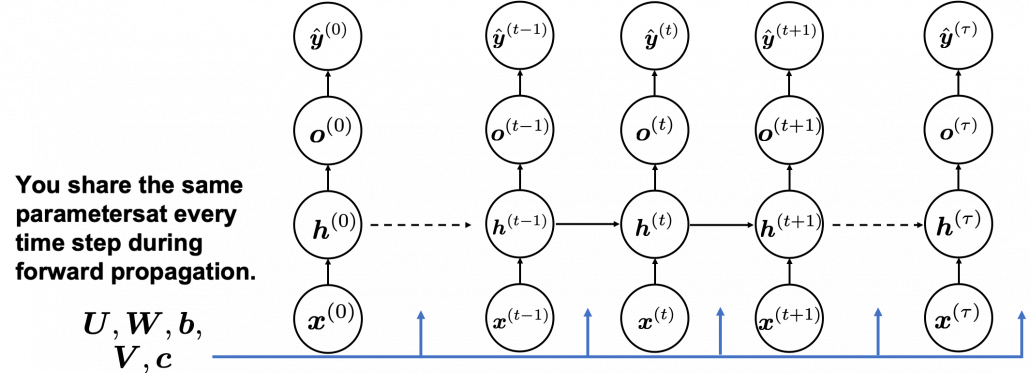
\includegraphics[width=\textwidth, height=0.4\textheight]{figure/S-RNN}
    \caption{S-RNN架构（展开形式，偏置向量被省去）}\label{fig:figuresrnn}
\end{figure}
\end{frame}

\begin{frame}\frametitle{S-RNN的局限性}
\small
\textbf{表现：难以捕获长期依赖}\footcite{zhang2023dive}
\begin{equation*}
    \symbf{h}_t = \tanh\left(\symbf{U} \symbf{h}_{t-1} + \symbf{W} \symbf{x}_t + \symbf{b}\right), \quad t=1,\ldots,T
\end{equation*}
同一组参数 $(\symbf{U},\symbf{W},\symbf{b})$ 在每个时间步重复使用：第 $j$ 步的输入要影响第 $t$ 步（$t\gg j$）的输出，必须连续经过 $t-j$ 次上述非线性变换，其影响通常随距离增大被逐步稀释——模型实际上只“记得住”近期信息.
\begin{figure}
  \centering
  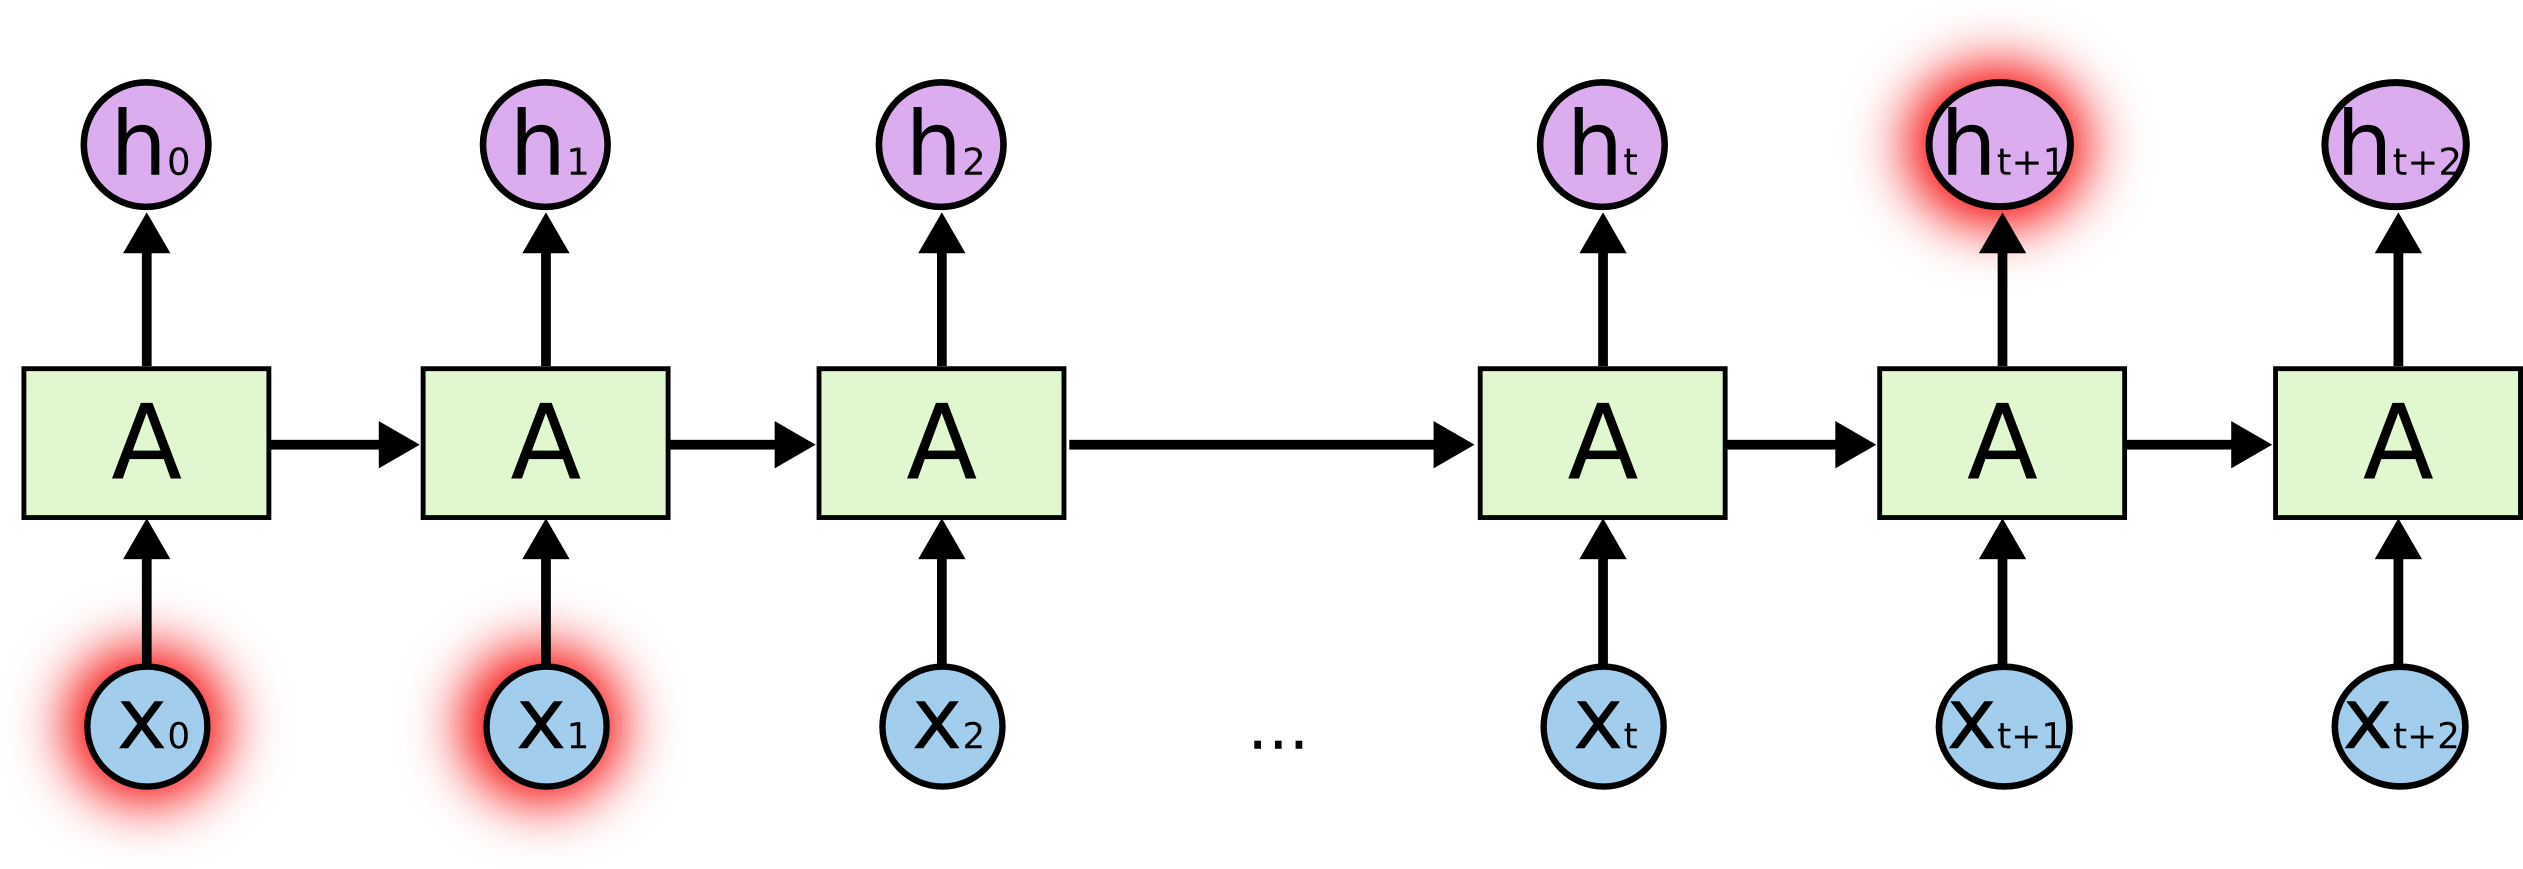
\includegraphics[width=0.8\textwidth, height=0.2\textheight]{figure/RNN-longtermdependencies}
  \caption{RNN 难以捕获长期依赖的示意}
\end{figure}
\textbf{机理：沿时间回传的梯度呈指数级衰减或增长}

记 $\delta\symbf{s}_t=\partial L/\partial\symbf{s}_t$（$\symbf{s}_t$ 为上页的输出层 logits），则损失对隐状态的梯度沿时间反向递推为
$\delta\symbf{h}_{t-1}=\symbf{A}_{t}\,\delta\symbf{h}_{t}+\symbf{V}^{\top}\delta\symbf{s}_{t-1}$，其中
    \begin{align*}
        \symbf{A}_{t} = \symbf{U}^{\top}\operatorname{diag}\left(\symbf{1} - \tanh^{2}(\symbf{r}_{t})\right)
    \end{align*}
其中 $\symbf{1}$ 为全 $1$ 向量，$\tanh^2$ 逐元素作用.跨越 $t-j$ 步的齐次部分为连乘 $\symbf{A}_{j+1}\symbf{A}_{j+2}\cdots\symbf{A}_{t}$.因每一步都含同一矩阵 $\symbf{U}^{\top}$，连乘接近矩阵的连续自乘，其范数随步数呈指数级变化：持续小于 $1$ 时\textbf{梯度消失}——远处时间步收不到学习信号，正是上述“记不住长期依赖”的根源；持续大于 $1$ 时\textbf{梯度爆炸}——训练不稳定，须依赖梯度裁剪.$\tanh$ 饱和区导数趋零会进一步加剧衰减.
\end{frame}

\subsection{经典LSTM架构}
\begin{frame}{经典LSTM架构概述：从S-RNN到LSTM}
\small
\begin{figure}[H]
    \centering
    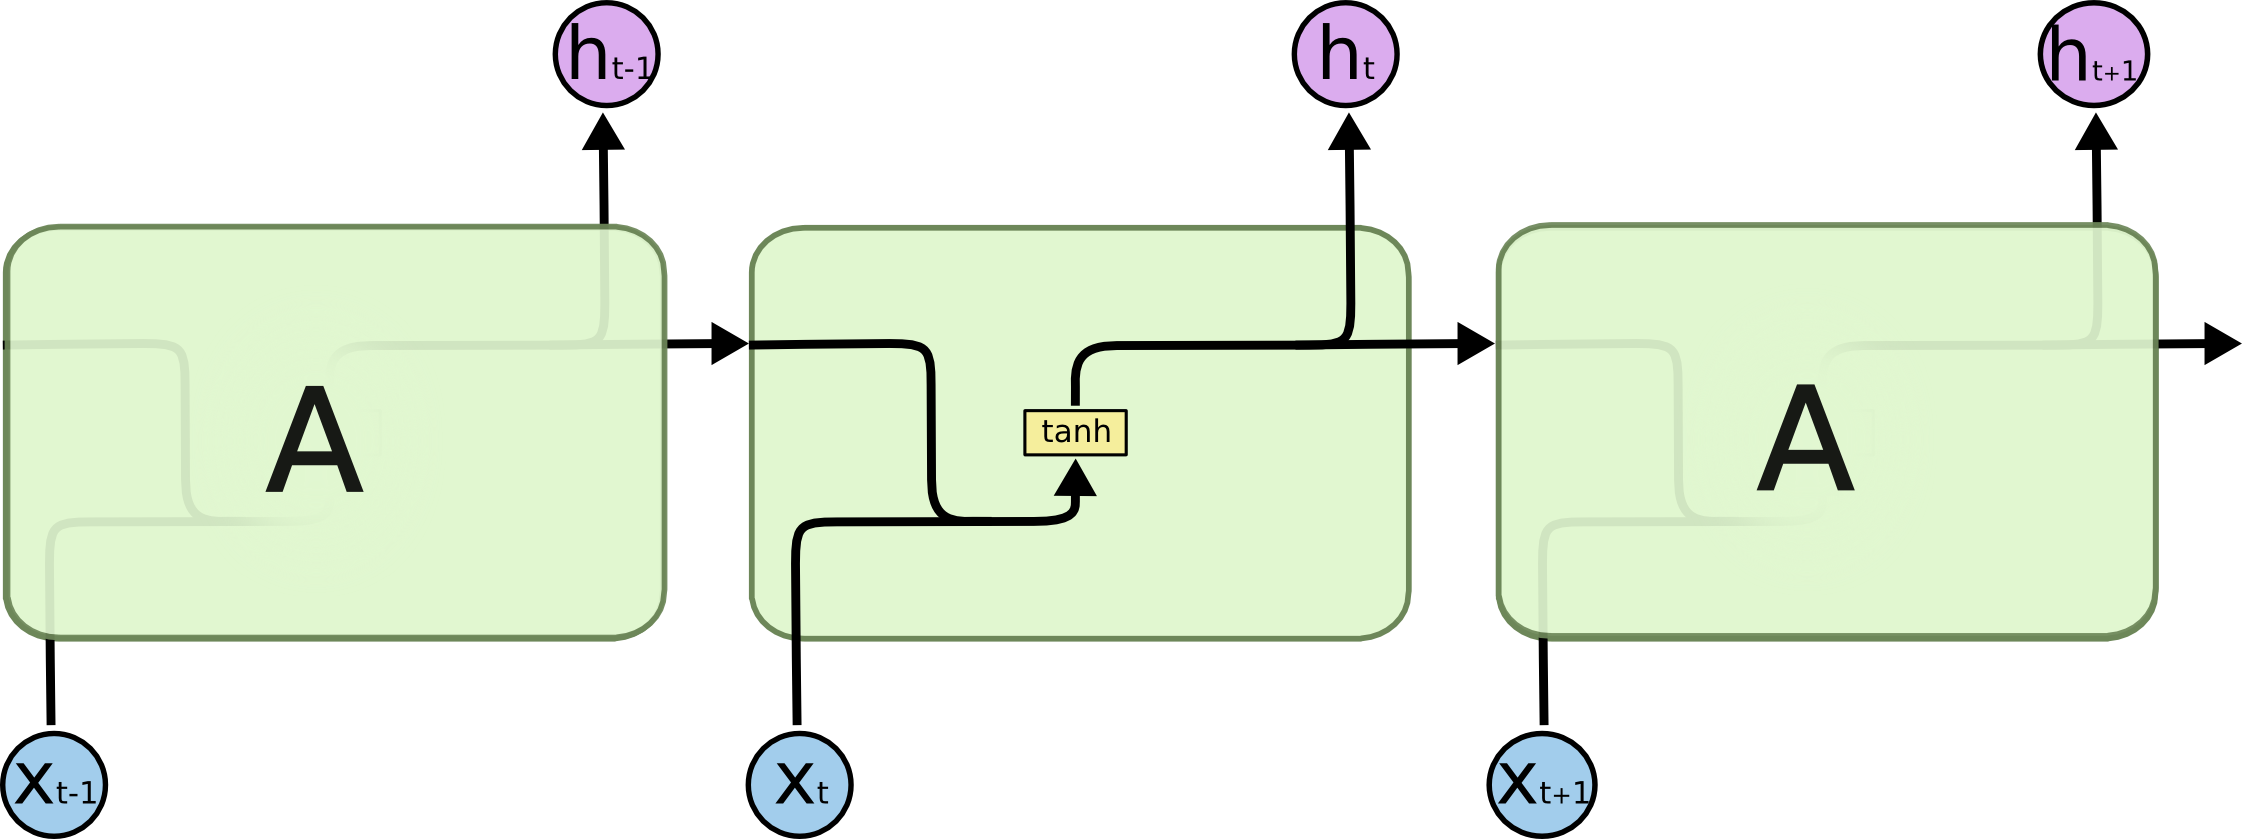
\includegraphics[width=0.85\textwidth, height=0.18\textheight]{figure/LSTM3-SimpleRNN}

    {\scriptsize \textbf{S-RNN重复模块}：仅单个$\tanh$层——隐状态是唯一的信息通道，每步被整体重写}

    \vspace{2pt}
    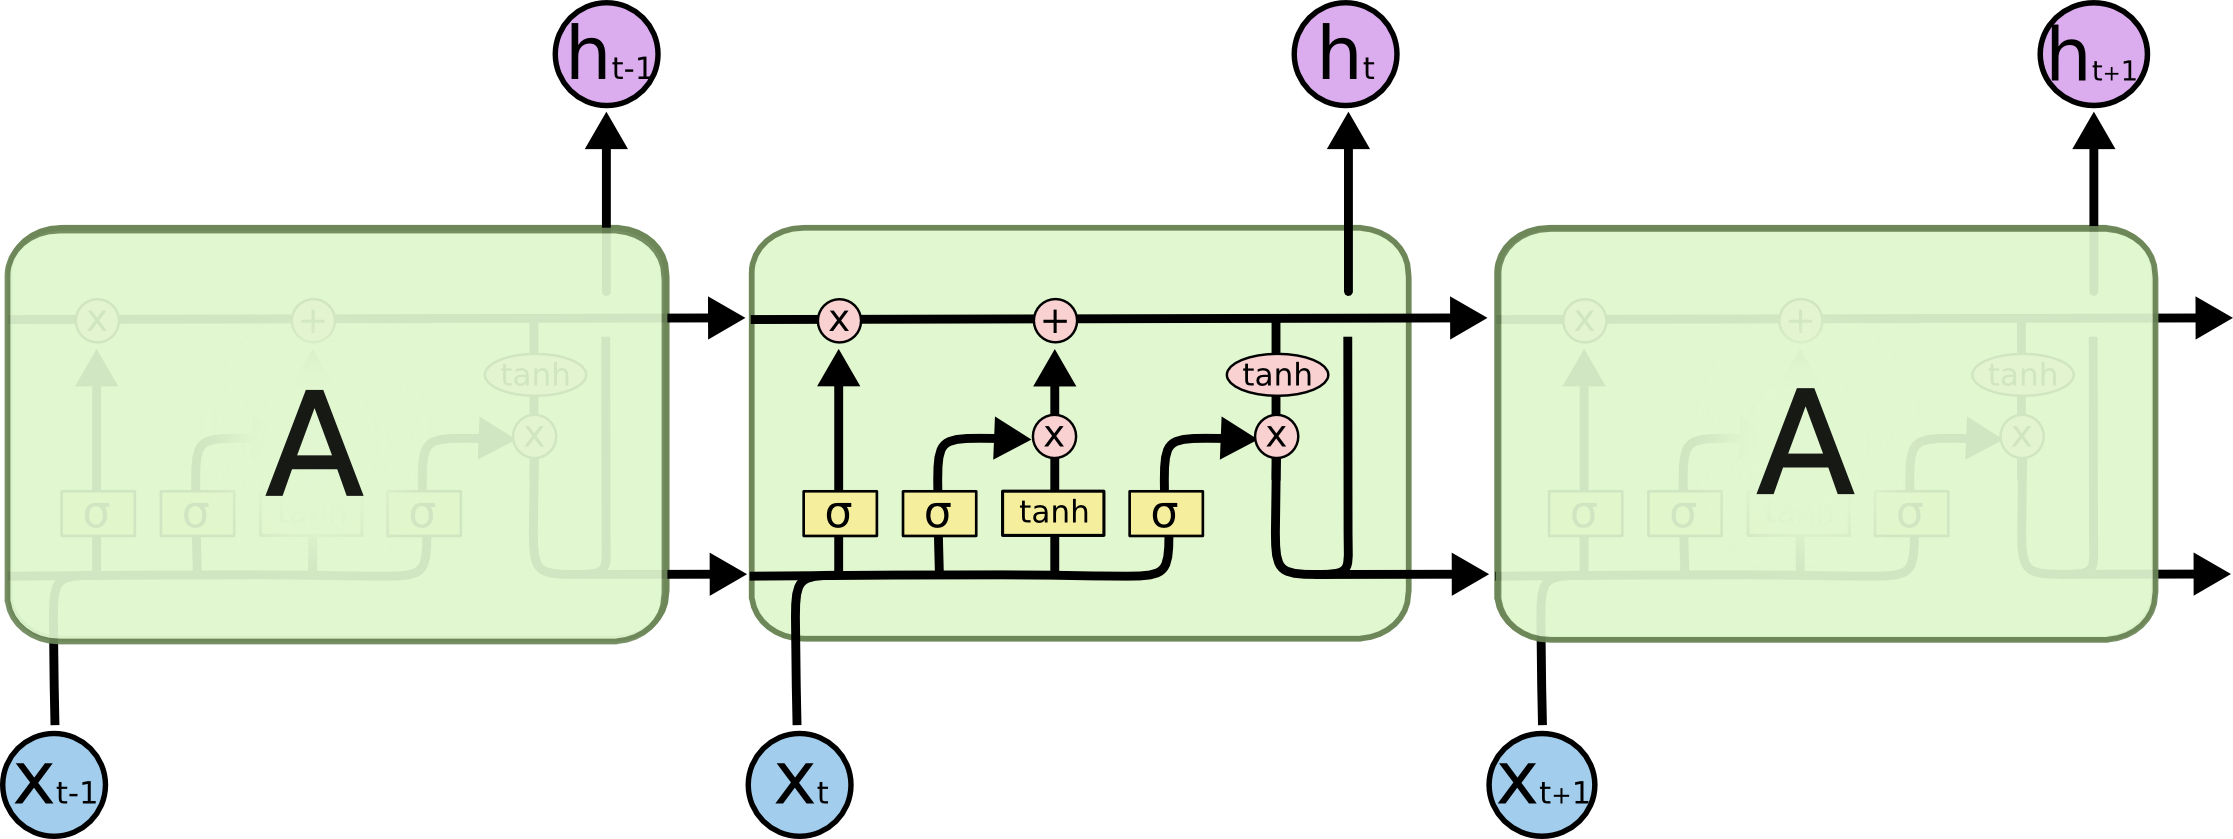
\includegraphics[width=0.85\textwidth, height=0.24\textheight]{figure/LSTM3-chain}

    {\scriptsize \textbf{LSTM重复模块}：细胞状态$\symbf{C}_t$横贯顶部（加性主路径），下方三个$\sigma$门管理其读写}
\end{figure}
长短期记忆网络（Long Short-Term Memory, LSTM）\footcite{SmirkCao}的两处关键改造：
\begin{enumerate}
    \item \textbf{记忆与输出分离}：增设细胞状态$\symbf{C}_t$专司长期记忆，沿加性路径平缓演化；隐状态$\symbf{h}_t$转为“工作记忆”，每步从$\symbf{C}_t$中按需提取；
    \item \textbf{从“无条件重写”到“门控读写”}：记忆的清除、写入、读出分别交由三个门显式控制——\textbf{遗忘门}（清除：丢弃哪些旧信息）、\textbf{输入门}（写入：纳入多少新信息）、\textbf{输出门}（读出：暴露多少记忆为$\symbf{h}_t$）.
\end{enumerate}
\end{frame}
\begin{frame}{经典LSTM架构}
    \begin{figure}[H]
        \centering
        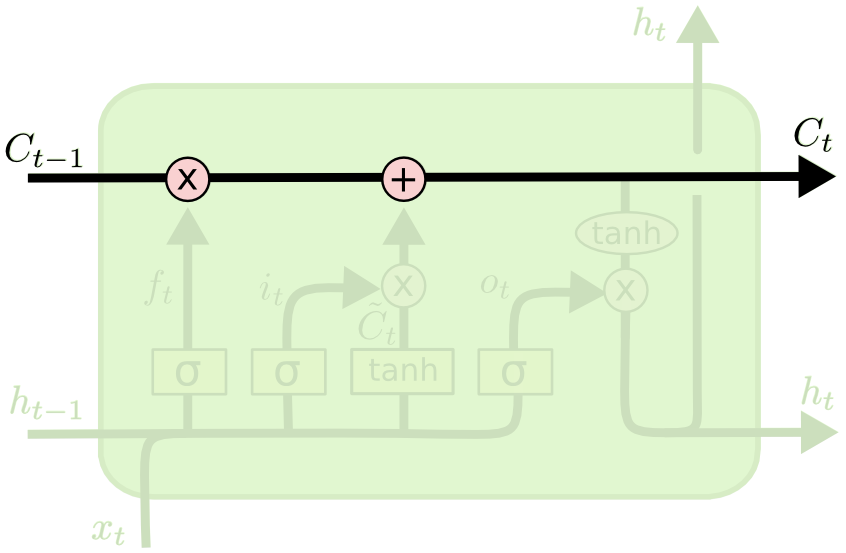
\includegraphics[width=\textwidth, height=0.4\textheight]{figure/LSTM3-C-line}
        \caption{LSTM 的细胞状态（长期记忆轨道）与隐状态（工作记忆）}
    \end{figure}
\begin{itemize}
    \item $\symbf{C}_{t}$（长期记忆轨道）：沿水平主路径只经历\textbf{逐元素缩放与加法}——不经过矩阵乘法，也不被$\tanh$之类的饱和函数反复挤压，信息得以低损耗地跨越长距离；
    \item $\symbf{h}_{t}$（工作记忆）：每步由输出门从$\tanh(\symbf{C}_t)$中\textbf{选择性提取}，直接参与当前输出与下一时刻的门控计算——变化快，只携带“此刻需要”的信息.
\end{itemize}
    \begin{figure}[H]
        \centering
        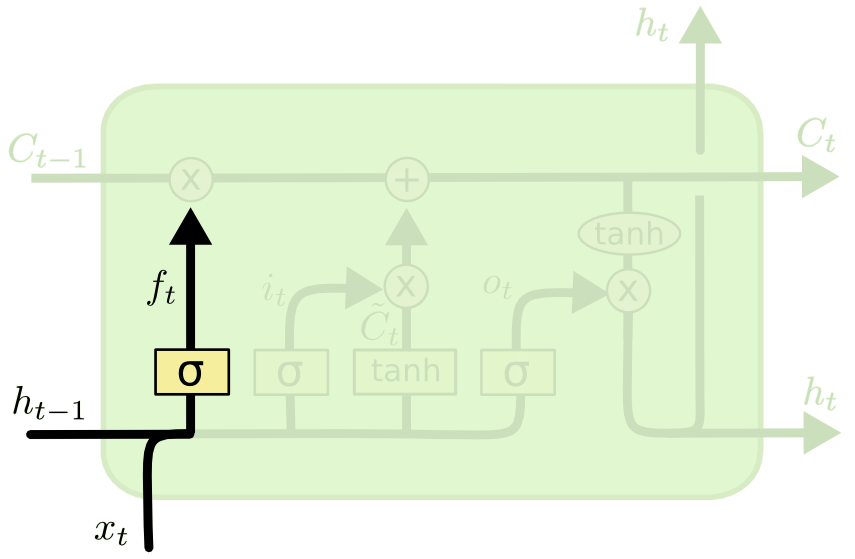
\includegraphics[width=\textwidth, height=0.4\textheight]{figure/LSTM3-focus-f}
        \caption{遗忘门：控制旧记忆 $\symbf{C}_{t-1}$ 的保留比例}
    \end{figure}
“遗忘门”基于$\symbf{h}_{t-1}$和$\symbf{x}_t$，得到各分量均在 $(0,1)$ 内的 $\symbf{f}_t$，逐维代表$\symbf{C}_{t-1}$中保留的比例：
    \begin{align*}
        \symbf{f}_t &= \sigma\left(\symbf{U}_f \symbf{h}_{t-1} + \symbf{W}_f \symbf{x}_t + \symbf{b}_f\right)
    \end{align*}

   \begin{figure}[H]
        \centering
        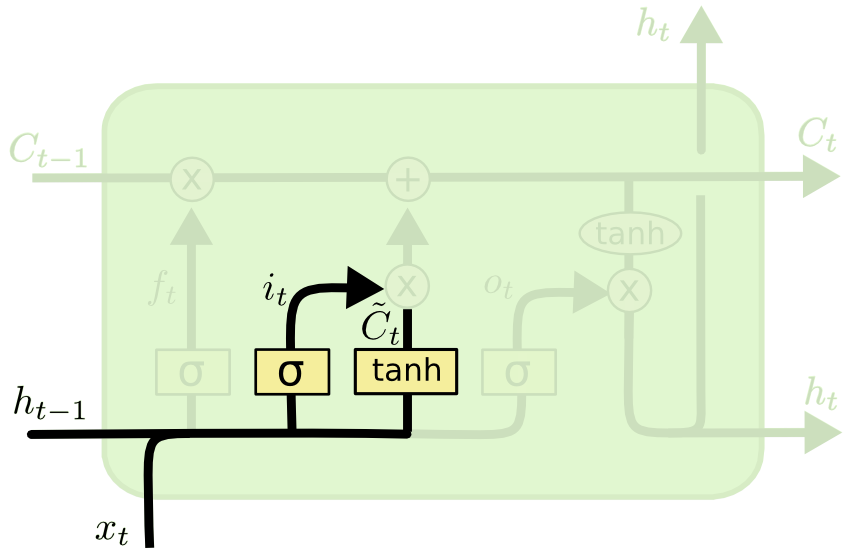
\includegraphics[width=\textwidth, height=0.4\textheight]{figure/LSTM3-focus-i}
        \caption{输入门：控制候选记忆 $\tilde{\symbf{C}}_t$ 的写入}
    \end{figure}
“输入门”基于$\symbf{h}_{t-1}$和$\symbf{x}_t$，得到新的记忆$\tilde{\symbf{C}}_t$和权重$\symbf{i}_{t}$：
    \begin{align*}
        \symbf{i}_t &= \sigma\left(\symbf{U}_i \symbf{h}_{t-1} + \symbf{W}_i \symbf{x}_t + \symbf{b}_i\right)\\
        \tilde{\symbf{C}}_t &= \tanh\left(\symbf{U}_c \symbf{h}_{t-1} + \symbf{W}_c \symbf{x}_t + \symbf{b}_c\right)
    \end{align*}
   \begin{figure}[H]
        \centering
        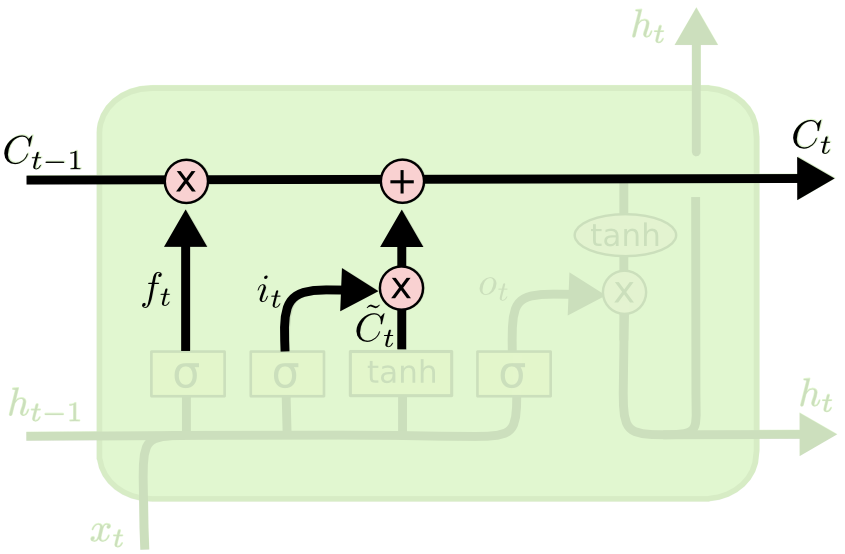
\includegraphics[width=\textwidth, height=0.4\textheight]{figure/LSTM3-focus-C}
        \caption{细胞状态更新：遗忘旧记忆并写入新记忆}
    \end{figure}
由已得的$\symbf{f}_t$和$\symbf{i}_t$，更新细胞状态$\symbf{C}_{t-1}$为$\symbf{C}_t$：
    \begin{align*}
        \symbf{C}_t &= \symbf{f}_t \odot \symbf{C}_{t-1} + \symbf{i}_t \odot \tilde{\symbf{C}}_t
    \end{align*}
\newpage
为分析长期记忆的梯度行为，重写上页的细胞状态更新式：
    \begin{align*}
        \symbf{C}_t &= \symbf{f}_t \odot \symbf{C}_{t-1} + \symbf{i}_t \odot \tilde{\symbf{C}}_t
    \end{align*}

沿细胞状态的直接加性路径（将$\symbf{f}_t,\symbf{i}_t,\tilde{\symbf{C}}_t$视为不依赖$\symbf{C}_{t-1}$的门控量）有 $\frac{\partial \symbf{C}_t}{\partial \symbf{C}_{t-1}}=\operatorname{diag}(\symbf{f}_t)$.

对照S-RNN：
\begin{align*}
    \symbf{A}_{t} = \symbf{U}^{\top}\operatorname{diag}\left(\symbf{1} - \tanh^{2}(\symbf{r}_{t})\right)
\end{align*}
跨步梯度由含固定矩阵$\symbf{U}^{\top}$的连乘$\prod_{j=1}^{k}\symbf{A}_{t+j}$决定，所有维度只能一同衰减或增长；这里跨$k$步的梯度系数为$\prod_{j=1}^{k}\operatorname{diag}(\symbf{f}_{t+j})$——\textbf{逐维独立、由数据驱动}：需要长期保留的维度可学得$f\approx 1$（梯度近似无衰减地跨越任意距离），应当遗忘的维度则学得$f\approx 0$.这条“可学习的选择性梯度通道”正是LSTM缓解长序列梯度消失的根本原因.
\newpage
    \begin{figure}[H]
        \centering
        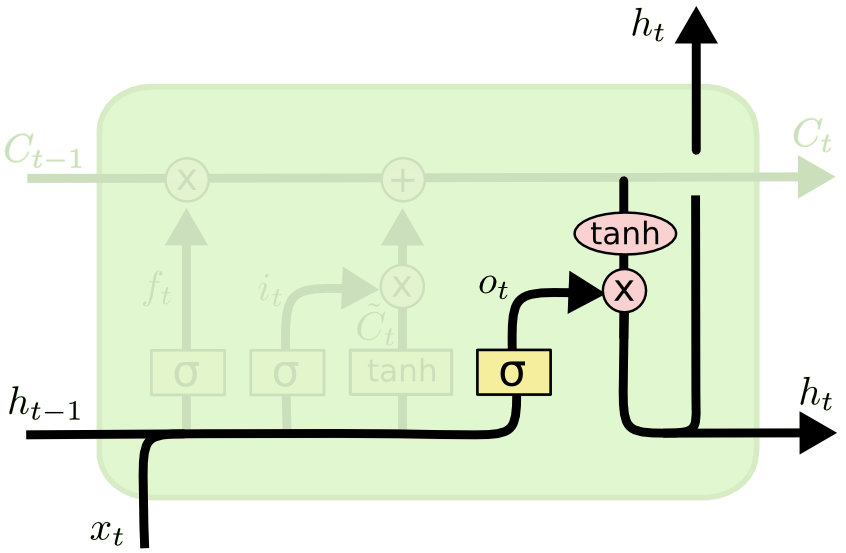
\includegraphics[width=\textwidth, height=0.4\textheight]{figure/LSTM3-focus-o}
        \caption{输出门：从细胞状态读出工作记忆 $\symbf{h}_t$}
    \end{figure}
“输出门”基于$\symbf{h}_{t-1}$和$\symbf{x}_t$，得到各分量均在 $(0,1)$ 内的权重$\symbf{o}_t$，随后与$\tanh$后的$\symbf{C}_t$逐元素相乘，得到更新后的短期记忆$\symbf{h}_t$，作为这一模块的输出：
    \begin{align*}
        \symbf{o}_t &= \sigma\left(\symbf{U}_o \symbf{h}_{t-1} + \symbf{W}_o \symbf{x}_t + \symbf{b}_o\right)\\
        \symbf{h}_t &= \symbf{o}_t \odot \tanh\left(\symbf{C}_t\right)
    \end{align*}
\newpage
\begin{columns}
  \column{0.5\textwidth}
\begin{figure}[H]
    \centering
    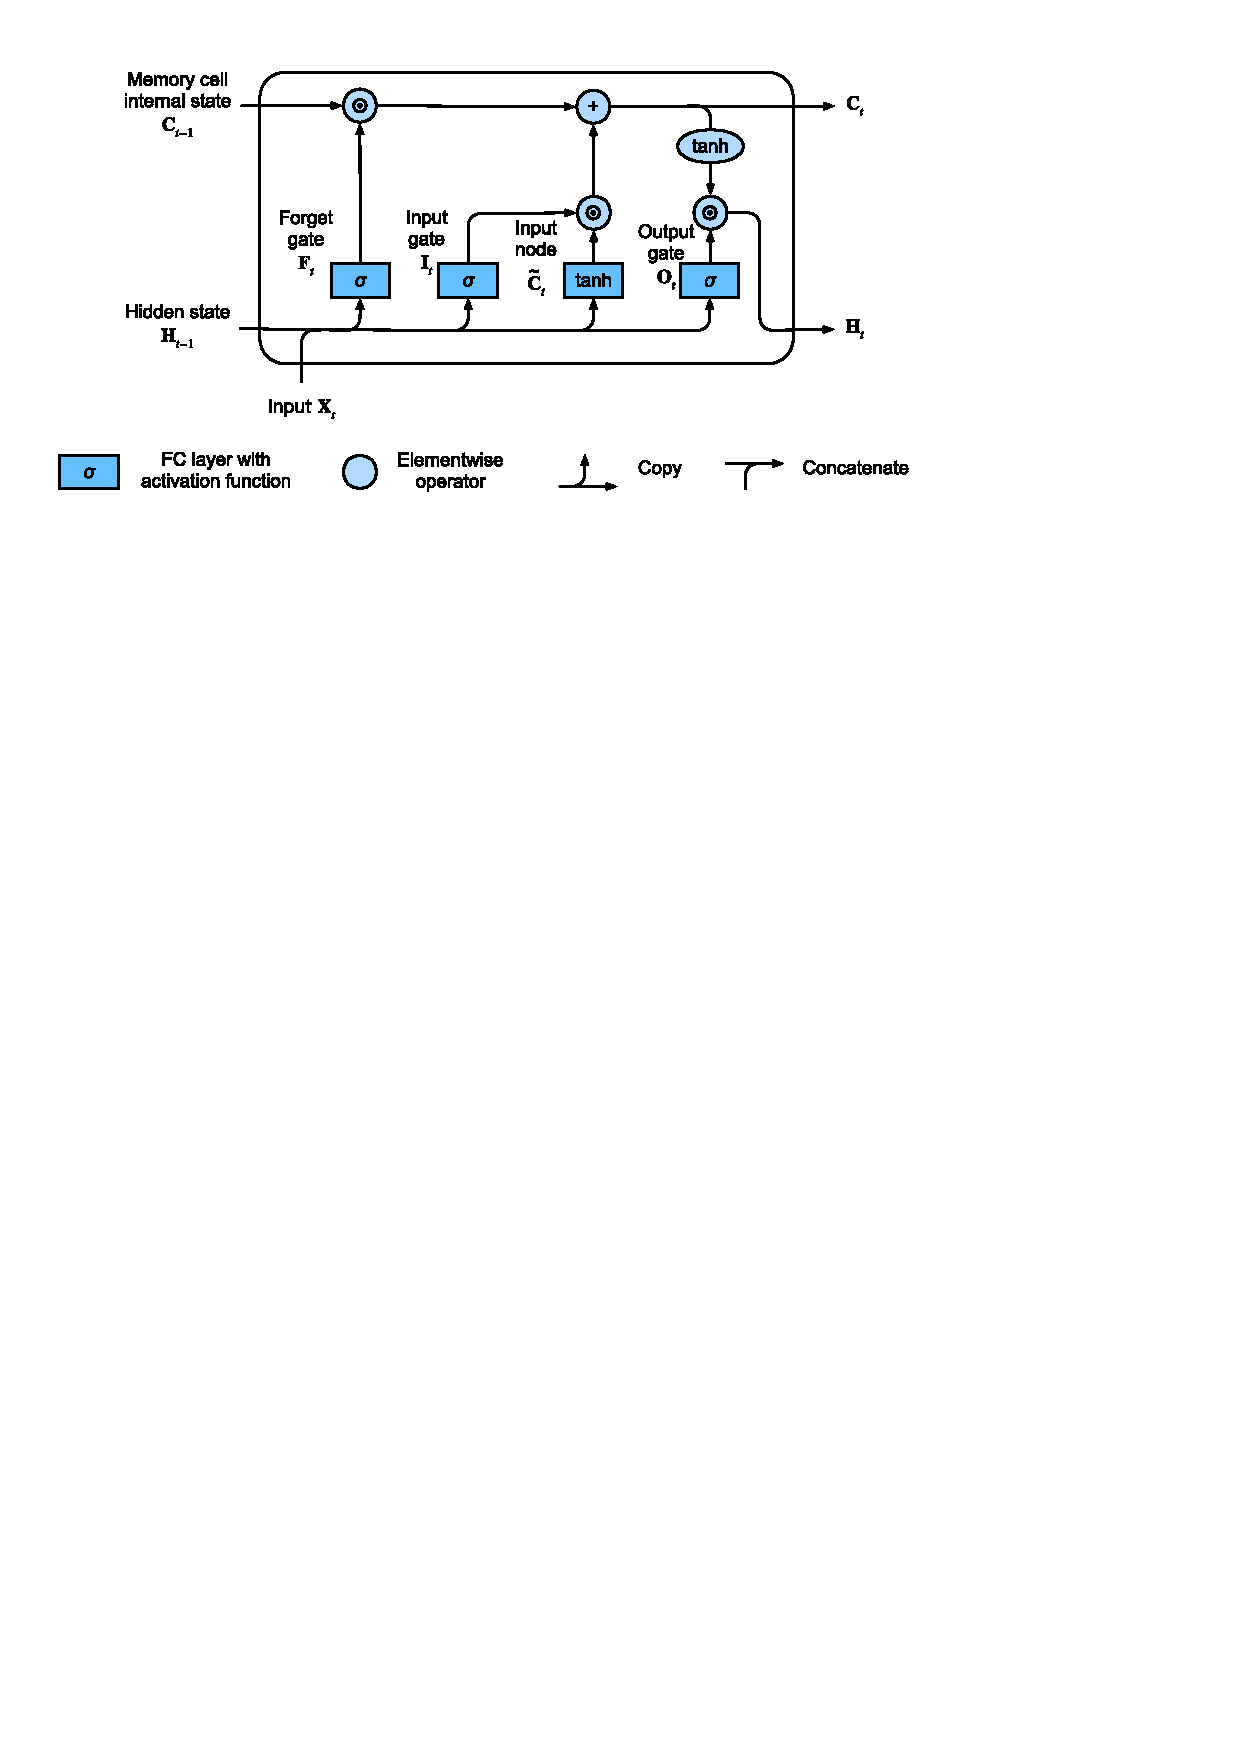
\includegraphics[width=\textwidth, height=0.3\textheight]{figure/lstm-3}
    \caption{经典 LSTM 单元的完整结构}
\end{figure}

  % 右侧：LSTM结构 Block
  \column{0.5\textwidth}
    \begin{align*}
        \symbf{f}_t &= \sigma (\symbf{U}_f \symbf{h}_{t-1} + \symbf{W}_f \symbf{x}_t + \symbf{b}_f)\\
        \symbf{i}_t &= \sigma (\symbf{U}_i \symbf{h}_{t-1} + \symbf{W}_i \symbf{x}_t + \symbf{b}_i)\\
        \symbf{o}_t &= \sigma (\symbf{U}_o \symbf{h}_{t-1} + \symbf{W}_o \symbf{x}_t + \symbf{b}_o)\\
        \tilde{\symbf{C}}_t &= \tanh (\symbf{U}_c \symbf{h}_{t-1} + \symbf{W}_c \symbf{x}_t + \symbf{b}_c)\\
        \symbf{C}_t &= \symbf{i}_t \odot \tilde{\symbf{C}}_t+\symbf{f}_t \odot \symbf{C}_{t-1}\\
        \symbf{h}_t &= \symbf{o}_t \odot \tanh(\symbf{C}_t)\\
        \hat{\symbf{y}}_{t} &= \mathrm{softmax}\left(\symbf{V} \symbf{h}_{t}+\symbf{c}\right)
    \end{align*}
\end{columns}
\end{frame}
\subsection{Peephole LSTM架构}
\begin{frame}{Peephole LSTM架构}
    \textbf{动机}：经典LSTM的三个门只能经$\symbf{h}_{t-1}=\symbf{o}_{t-1}\odot\tanh(\symbf{c}_{t-1})$\textbf{间接}感知记忆，一旦上一步输出门接近关闭（$\symbf{h}_{t-1}\approx\symbf{0}$），门控便对细胞状态“失明”.Peephole LSTM为此增加“\textbf{窥视孔连接}”，让门控\textbf{直接}读取细胞状态：输入门和遗忘门读取$\symbf{c}_{t-1}$，输出门读取更新后的$\symbf{c}_t$（最初被用于需要精确计时、计数的任务，如节奏识别）.
\begin{columns}
  \column{0.45\textwidth}
\begin{figure}[H]
    \centering
    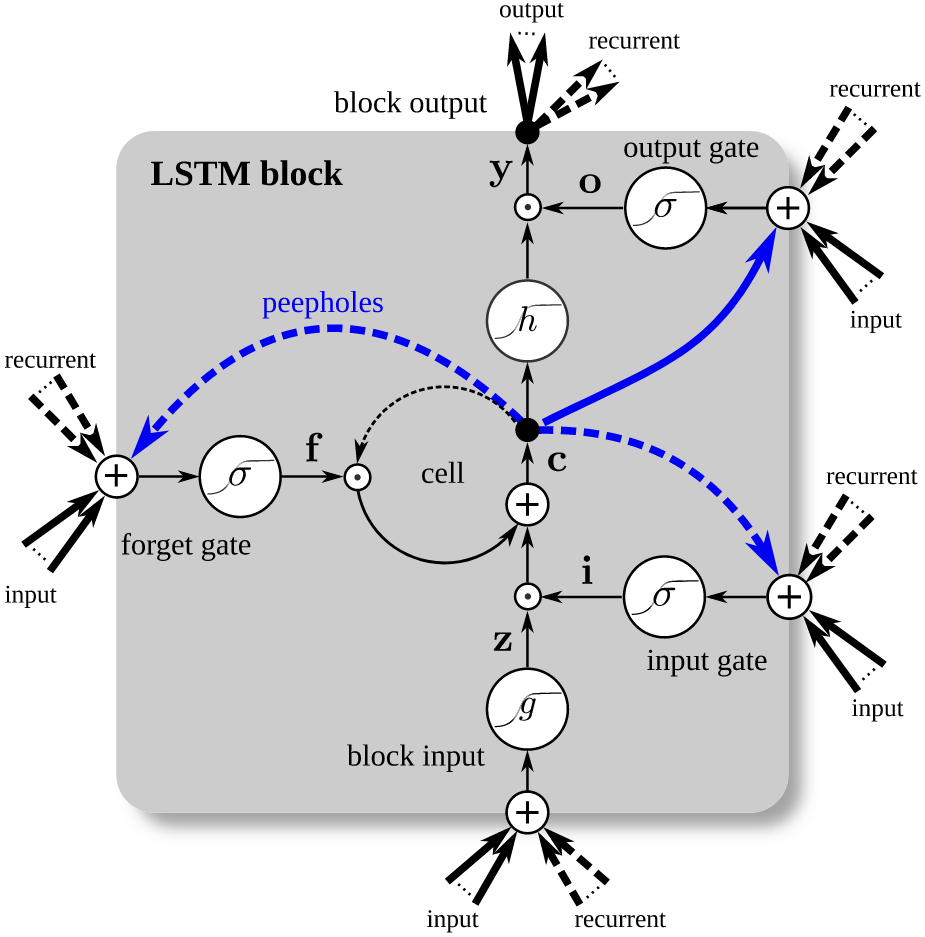
\includegraphics[width=\textwidth, height=0.46\textheight]{figure/LSTM block}
    \caption{Peephole LSTM 单元结构（含窥视孔连接）}
\end{figure}

  % 右侧：LSTM结构 Block
  \column{0.5\textwidth}
    \small
    \begin{align*}
        \symbf{z}_t &= \tanh\left(\symbf{U}_z \symbf{h}_{t-1} + \symbf{W}_z \symbf{x}_t + \symbf{b}_z\right)\\
        \symbf{i}_t &= \sigma\left(\symbf{U}_i \symbf{h}_{t-1} + \symbf{W}_i \symbf{x}_t + \symbf{p}_{i} \odot \symbf{c}_{t-1} + \symbf{b}_i\right) \\
        \symbf{f}_t &= \sigma\left(\symbf{U}_f \symbf{h}_{t-1} + \symbf{W}_f \symbf{x}_t + \symbf{p}_{f} \odot \symbf{c}_{t-1} + \symbf{b}_f\right) \\
        \symbf{c}_t &= \symbf{f}_t \odot \symbf{c}_{t-1} + \symbf{i}_t \odot \symbf{z}_t \\
        \symbf{o}_t &= \sigma\left(\symbf{U}_o \symbf{h}_{t-1} + \symbf{W}_o \symbf{x}_t + \symbf{p}_{o} \odot \symbf{c}_{t} + \symbf{b}_o\right) \\
        \symbf{h}_t &= \symbf{o}_t \odot \tanh\left(\symbf{c}_t\right)\\
        \hat{\symbf{y}}_{t} &= \mathrm{softmax}\left(\symbf{V}\symbf{h}_{t}+\symbf{b}_{y}\right)
    \end{align*}
    \scriptsize 注：输出层偏置记为$\symbf{b}_{y}$（即经典LSTM中的$\symbf{c}$），以免与细胞状态$\symbf{c}_t$混淆；候选记忆记为$\symbf{z}_t$，对应经典LSTM中的$\tilde{\symbf{C}}_t$.
\end{columns}
\end{frame}
\subsection{经典LSTM、Peephole LSTM对比}
\begin{frame}{经典LSTM、Peephole LSTM对比}
\begin{figure}[H]
    \centering
    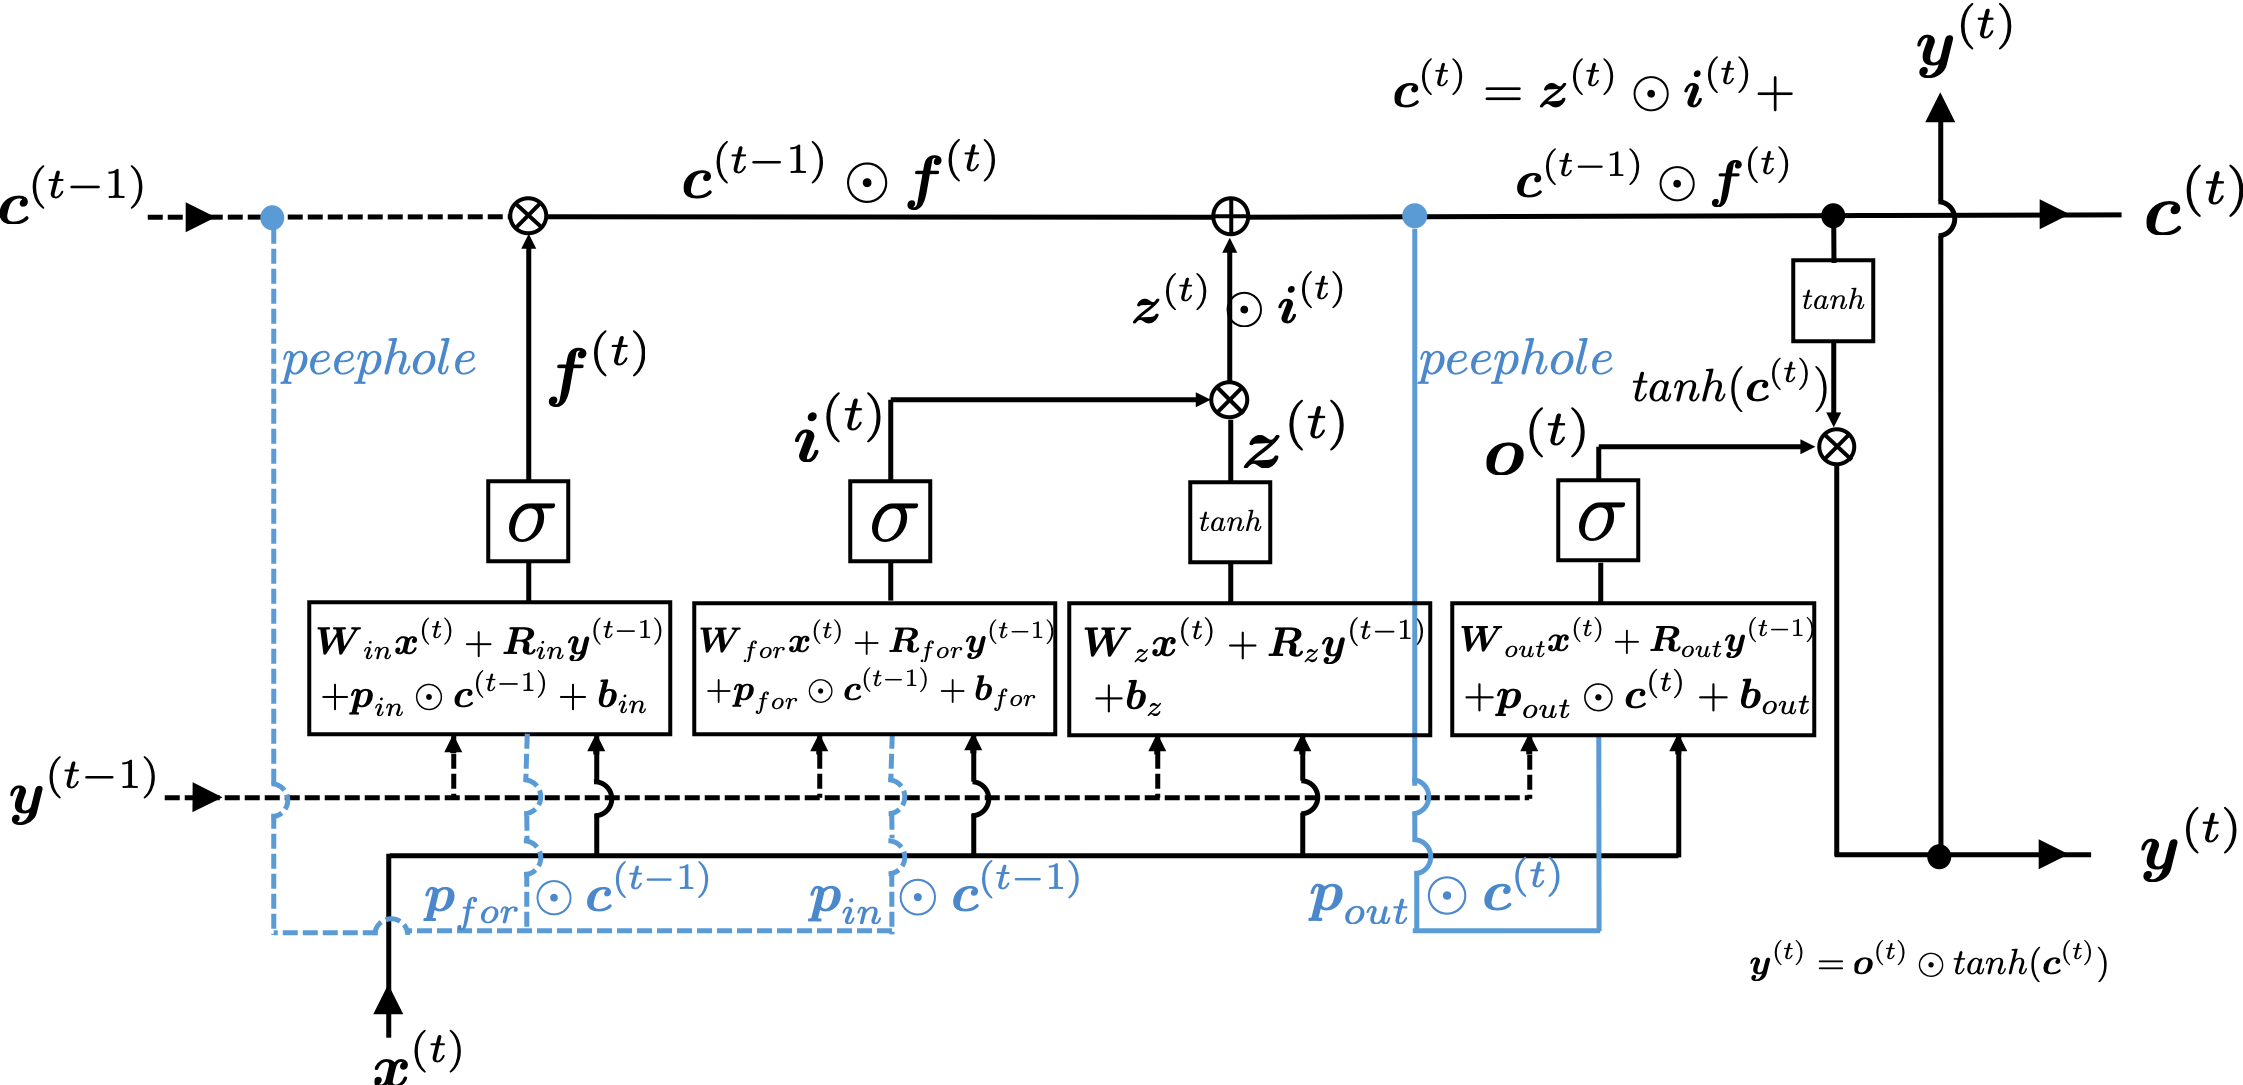
\includegraphics[width=\textwidth, height=0.65\textheight]{figure/peep-hole-LSTM}
    \caption{经典 LSTM 与 Peephole LSTM 的结构对比}
\end{figure}
\end{frame}
\subsection{经典LSTM反向传播理论}
\begin{frame}{经典LSTM反向传播理论}
    \begin{columns}
        \column{0.5\textwidth}
\begin{figure}[H]
    \centering
    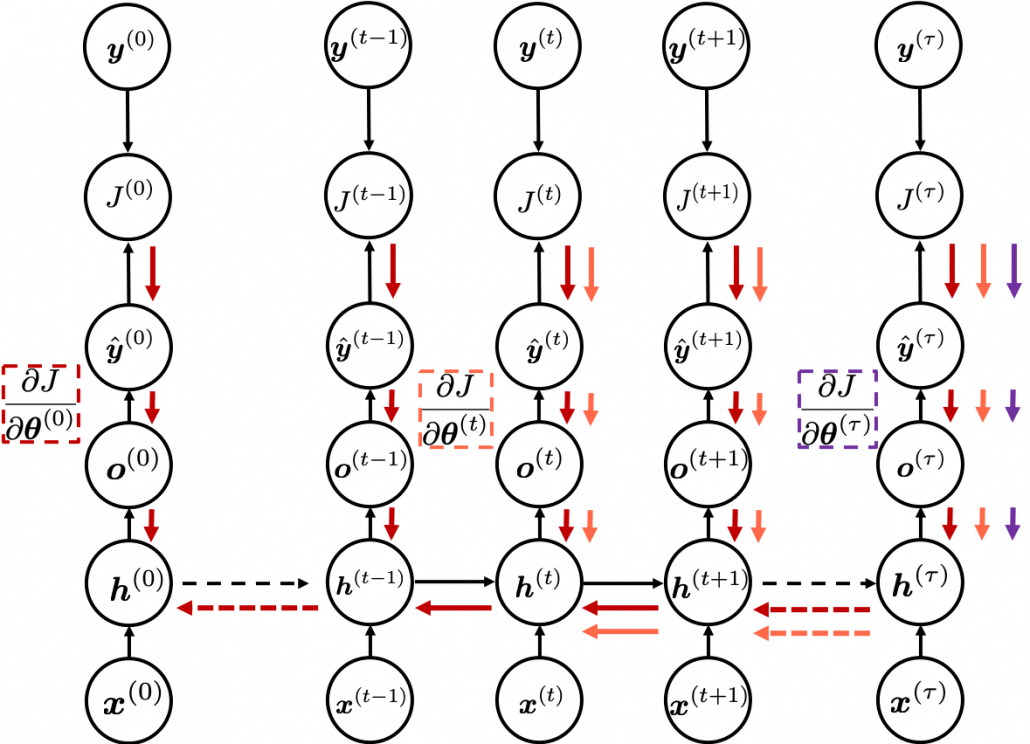
\includegraphics[width=\textwidth, height=0.5\textheight]{figure/LSTM反向传播}
    \caption{LSTM 沿时间反向传播的梯度流}
\end{figure}
  \column{0.5\textwidth}
    \begin{align*}
        \symbf{f}_t &= \sigma (\symbf{U}_f \symbf{h}_{t-1} + \symbf{W}_f \symbf{x}_t + \symbf{b}_f)\\
        \symbf{i}_t &= \sigma (\symbf{U}_i \symbf{h}_{t-1} + \symbf{W}_i \symbf{x}_t + \symbf{b}_i)\\
        \symbf{o}_t &= \sigma (\symbf{U}_o \symbf{h}_{t-1} + \symbf{W}_o \symbf{x}_t + \symbf{b}_o)\\
        \tilde{\symbf{C}}_t &= \tanh (\symbf{U}_c \symbf{h}_{t-1} + \symbf{W}_c \symbf{x}_t + \symbf{b}_c)\\
        \symbf{C}_t &= \symbf{f}_t \odot \symbf{C}_{t-1}+\symbf{i}_t \odot \tilde{\symbf{C}}_t\\
        \symbf{h}_t &= \symbf{o}_t \odot \tanh(\symbf{C}_t)\\
        \hat{\symbf{y}}_{t} &= \mathrm{softmax}\left(\symbf{V} \symbf{h}_{t}+\symbf{c}\right)
    \end{align*}
\end{columns}
\end{frame}
\begin{frame}{经典LSTM反向传播理论推导}
\scriptsize
\setlength{\abovedisplayskip}{3pt}\setlength{\belowdisplayskip}{3pt}%
\setlength{\abovedisplayshortskip}{1pt}\setlength{\belowdisplayshortskip}{1pt}%
\begin{columns}[T,onlytextwidth]
  \column{0.44\textwidth}
  \textbf{前向（求导依据）}\par\smallskip
  预激活量（$*\in\{f,i,o,c\}$）：
  \[\bar{\symbf{g}}_{*,t}=\symbf{U}_*\symbf{h}_{t-1}+\symbf{W}_*\symbf{x}_t+\symbf{b}_*\]
  \begin{align*}
    \symbf{f}_t&=\sigma(\bar{\symbf{f}}_t),\quad \symbf{i}_t=\sigma(\bar{\symbf{i}}_t)\\
    \symbf{o}_t&=\sigma(\bar{\symbf{o}}_t),\quad \tilde{\symbf{C}}_t=\tanh(\bar{\symbf{C}}_t)\\
    \symbf{C}_t&=\symbf{f}_t\odot\symbf{C}_{t-1}+\symbf{i}_t\odot\tilde{\symbf{C}}_t\\
    \symbf{h}_t&=\symbf{o}_t\odot\tanh(\symbf{C}_t)\\
    \symbf{s}_t&=\symbf{V}\symbf{h}_t+\symbf{c},\quad \hat{\symbf{y}}_t=\mathrm{softmax}(\symbf{s}_t)
  \end{align*}
  \textbf{依据要点}：损失项 $\delta\symbf{s}_t=\hat{\symbf{y}}_t-\symbf{y}_t$（第 $t$ 步参与损失，否则取 $\symbf{0}$）.边界 $\symbf{C}_0=\symbf{h}_0=\symbf{0}$，且
  $\delta\symbf{C}_{\tau+1}=\delta\bar{\symbf{f}}_{\tau+1}=\delta\bar{\symbf{i}}_{\tau+1}=\delta\bar{\symbf{o}}_{\tau+1}=\delta\bar{\symbf{C}}_{\tau+1}=\symbf{0}$，从 $t=\tau$ 到 $1$ 反向递推.

  \vspace{3em}
  \column{0.54\textwidth}
  \textbf{反向推导}
  \begin{align*}
    \delta\symbf{h}_t &= \symbf{V}^{\top}\delta\symbf{s}_t
      + \symbf{U}_f^{\top}\delta\bar{\symbf{f}}_{t+1}
      + \symbf{U}_i^{\top}\delta\bar{\symbf{i}}_{t+1}\\
    &\quad + \symbf{U}_o^{\top}\delta\bar{\symbf{o}}_{t+1}
      + \symbf{U}_c^{\top}\delta\bar{\symbf{C}}_{t+1}\\
    \delta\symbf{C}_t &= \delta\symbf{h}_t\odot\symbf{o}_t\odot(1-\tanh^2\!\symbf{C}_t)
      + \delta\symbf{C}_{t+1}\odot\symbf{f}_{t+1}\\
    \delta\bar{\symbf{o}}_t &= \delta\symbf{h}_t\odot\tanh(\symbf{C}_t)\odot\symbf{o}_t\odot(1-\symbf{o}_t)\\
    \delta\bar{\symbf{f}}_t &= \delta\symbf{C}_t\odot\symbf{C}_{t-1}\odot\symbf{f}_t\odot(1-\symbf{f}_t)\\
    \delta\bar{\symbf{i}}_t &= \delta\symbf{C}_t\odot\tilde{\symbf{C}}_t\odot\symbf{i}_t\odot(1-\symbf{i}_t)\\
    \delta\bar{\symbf{C}}_t &= \delta\symbf{C}_t\odot\symbf{i}_t\odot(1-\tilde{\symbf{C}}_t^2)
  \end{align*}
  共享参数梯度（$\bar{\symbf{g}}_{c,t}=\bar{\symbf{C}}_t$）：
  \begin{align*}
    \frac{\partial L}{\partial \symbf{U}_{*}}&=\textstyle\sum_{t}\delta\bar{\symbf{g}}_{*,t}\symbf{h}_{t-1}^{\top}, &
    \frac{\partial L}{\partial \symbf{W}_{*}}&=\textstyle\sum_{t}\delta\bar{\symbf{g}}_{*,t}\symbf{x}_{t}^{\top}\\
    \frac{\partial L}{\partial \symbf{b}_{*}}&=\textstyle\sum_{t}\delta\bar{\symbf{g}}_{*,t}, &
    \frac{\partial L}{\partial \symbf{V}}&=\textstyle\sum_{t}\delta\symbf{s}_t \symbf{h}_t^{\top}\\
    \frac{\partial L}{\partial \symbf{c}}&=\textstyle\sum_{t}\delta\symbf{s}_t
  \end{align*}
\end{columns}
\par\smallskip
{\scriptsize 左栏前向式即右栏每步求导的依据；该形式避免将输出门 $\symbf{o}_t$ 与分类 logits $\symbf{s}_t$ 混用，多分类对应 softmax 交叉熵，二分类可视作两类 softmax.}
\end{frame}

\subsection{Peephole LSTM反向传播理论}
\begin{frame}{Peephole LSTM反向传播理论}
\scriptsize
\setlength{\abovedisplayskip}{3pt}\setlength{\belowdisplayskip}{3pt}%
\setlength{\abovedisplayshortskip}{1pt}\setlength{\belowdisplayshortskip}{1pt}%
\begin{columns}[T,onlytextwidth]
  \column{0.44\textwidth}
  \textbf{前向（求导依据）}\par\smallskip
  预激活量 $\bar{\symbf{g}}_{*,t}=\symbf{U}_*\symbf{h}_{t-1}+\symbf{W}_*\symbf{x}_t+\symbf{b}_*$；门控另含\textbf{窥视孔项}——$\bar{\symbf{i}}_t,\bar{\symbf{f}}_t$ 加 $\symbf{p}_i,\symbf{p}_f$ 与 $\symbf{c}_{t-1}$ 的逐元素积，$\bar{\symbf{o}}_t$ 加 $\symbf{p}_o\odot\symbf{c}_t$，$\bar{\symbf{z}}_t$ 无.
  \begin{align*}
    \symbf{z}_t&=\tanh(\bar{\symbf{z}}_t),\quad \symbf{i}_t=\sigma(\bar{\symbf{i}}_t)\\
    \symbf{f}_t&=\sigma(\bar{\symbf{f}}_t),\quad \symbf{o}_t=\sigma(\bar{\symbf{o}}_t)\\
    \symbf{c}_t&=\symbf{f}_t\odot\symbf{c}_{t-1}+\symbf{i}_t\odot\symbf{z}_t\\
    \symbf{h}_t&=\symbf{o}_t\odot\tanh(\symbf{c}_t)
  \end{align*}
  \textbf{依据要点}：$\symbf{p}_i\odot\symbf{c}_{t-1},\ \symbf{p}_f\odot\symbf{c}_{t-1},\ \symbf{p}_o\odot\symbf{c}_t$ 为门控\textbf{直接}读取 $\symbf{c}$ 的窥视孔路径，使 $\delta\symbf{c}_t$ 较经典情形多出三项.边界项约定同经典，且 $\symbf{c}_0=\symbf{h}_0=\symbf{0}$.

  \vspace{3em}
  \column{0.54\textwidth}
  \textbf{反向推导（增设窥视孔路径）}
  \begin{align*}
    \delta\symbf{h}_t &= \symbf{V}^{\top}\delta\symbf{s}_t
      +\symbf{U}_z^{\top}\delta\bar{\symbf{z}}_{t+1}
      +\symbf{U}_i^{\top}\delta\bar{\symbf{i}}_{t+1}\\
    &\quad +\symbf{U}_f^{\top}\delta\bar{\symbf{f}}_{t+1}
      +\symbf{U}_o^{\top}\delta\bar{\symbf{o}}_{t+1}\\
    \delta\symbf{c}_t &= \delta\symbf{h}_t\odot\symbf{o}_t\odot(1-\tanh^2\!\symbf{c}_t)
      +\delta\symbf{c}_{t+1}\odot\symbf{f}_{t+1}\\
    &\quad +\underbrace{\symbf{p}_o\odot\delta\bar{\symbf{o}}_t
      +\symbf{p}_i\odot\delta\bar{\symbf{i}}_{t+1}
      +\symbf{p}_f\odot\delta\bar{\symbf{f}}_{t+1}}_{\text{窥视孔新增项}}\\
    \delta\bar{\symbf{o}}_t &= \delta\symbf{h}_t\odot\tanh(\symbf{c}_t)\odot\symbf{o}_t\odot(1-\symbf{o}_t)\\
    \delta\bar{\symbf{f}}_t &= \delta\symbf{c}_t\odot\symbf{c}_{t-1}\odot\symbf{f}_t\odot(1-\symbf{f}_t)\\
    \delta\bar{\symbf{i}}_t &= \delta\symbf{c}_t\odot\symbf{z}_t\odot\symbf{i}_t\odot(1-\symbf{i}_t)\\
    \delta\bar{\symbf{z}}_t &= \delta\symbf{c}_t\odot\symbf{i}_t\odot(1-\symbf{z}_t^2)
  \end{align*}
  权重梯度（$*\in\{z,i,f,o\}$）：
  \begin{align*}
    \frac{\partial L}{\partial\symbf{U}_*}&=\textstyle\sum_t\delta\bar{\symbf{g}}_{*,t}\symbf{h}_{t-1}^{\top}, &
    \frac{\partial L}{\partial\symbf{W}_*}&=\textstyle\sum_t\delta\bar{\symbf{g}}_{*,t}\symbf{x}_t^{\top}\\
    \frac{\partial L}{\partial\symbf{b}_*}&=\textstyle\sum_t\delta\bar{\symbf{g}}_{*,t}, &
    \frac{\partial L}{\partial\symbf{p}_i}&=\textstyle\sum_t\delta\bar{\symbf{i}}_t\odot\symbf{c}_{t-1}\\
    \frac{\partial L}{\partial\symbf{p}_f}&=\textstyle\sum_t\delta\bar{\symbf{f}}_t\odot\symbf{c}_{t-1}, &
    \frac{\partial L}{\partial\symbf{p}_o}&=\textstyle\sum_t\delta\bar{\symbf{o}}_t\odot\symbf{c}_t
  \end{align*}
  \smallskip
  {\scriptsize $\delta\bar{\symbf{g}}_{*,t}$ 分别对应 $\delta\bar{\symbf{z}}_t,\delta\bar{\symbf{i}}_t,\delta\bar{\symbf{f}}_t,\delta\bar{\symbf{o}}_t$；输出层参数 $\symbf{V},\symbf{b}_{y}$ 的梯度与经典 LSTM 中 $\symbf{V},\symbf{c}$ 同形.}
\end{columns}
\end{frame}
\section{CNN简要原理}
\subsection{概述}
\begin{frame}\frametitle{卷积神经网络的概述}
卷积神经网络（Convolutional Neural Network, CNN）是一种特殊的前馈神经网络，其名称来源于其核心操作——卷积.

卷积神经网络的核心结构通常包括卷积层、非线性层、池化层以及用于任务输出的全连接层.

与全连接网络相比，卷积层内含两大\textbf{归纳偏置}：\textbf{局部连接}（每个输出只依赖输入的一个小邻域）与\textbf{权重共享}（同一卷积核在所有位置复用）.二者使参数量与输入尺寸解耦，并赋予特征提取\textbf{平移等变性}——同一模式无论出现在何处都由同一组权重检测；再配合池化，可进一步获得对小幅位移的不变性.后文将看到，这一偏置恰好契合文本分类中“关键短语在哪都算数”的任务结构.
\begin{figure}[H]
    \centering
    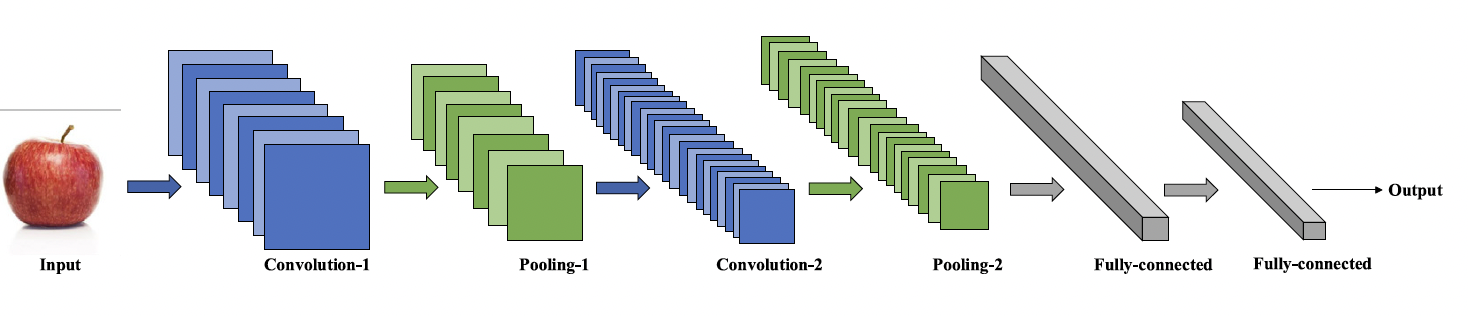
\includegraphics[width=\textwidth]{fig/cnn结构}
    \caption{卷积神经网络的基本结构}\label{fig:figurecnn}
\end{figure}

\end{frame}
\subsection{输入层}
\begin{frame}\frametitle{输入层}
\begin{minipage}[H]{0.4\textwidth}
    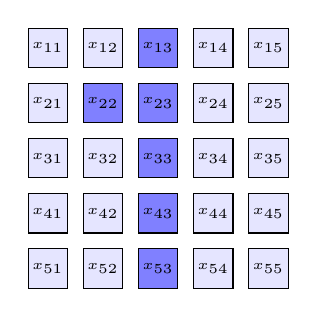
\begin{tikzpicture}[every node/.style={inner sep=0pt,outer sep=0pt},font=\tiny,scale=1,transform shape]
        % 输入层:5x5矩阵
        \foreach \x in {1,...,5} {
            \foreach \y in {1,...,5} {
                % 条件判断:特定位置为深色
                \ifnum\x=3
                    \node[draw,fill=blue!50,minimum size=0.5cm] (input-\x-\y) at (\x*0.7,-\y*0.7) {$x_{\y\x}$};
                \else
                    \ifnum\y=2 \ifnum\x=2
                        \node[draw,fill=blue!50,minimum size=0.5cm] (input-\x-\y) at (\x*0.7,-\y*0.7) {$x_{\y\x}$};
                    \else
                        \node[draw,fill=blue!10,minimum size=0.5cm] (input-\x-\y) at (\x*0.7,-\y*0.7) {$x_{\y\x}$};
                    \fi
                    \else
                        \node[draw,fill=blue!10,minimum size=0.5cm] (input-\x-\y) at (\x*0.7,-\y*0.7) {$x_{\y\x}$};
                    \fi
                \fi
            }
        }
    \end{tikzpicture}
    \label{fig:input-image}
\end{minipage}%
\hspace{0.2cm}
\begin{minipage}[H]{0.4\textwidth}
    \centering
    \[
    \begin{pmatrix}
        x_{11} & x_{12} & x_{13} & x_{14} & x_{15}\\
        x_{21} & x_{22} & x_{23} & x_{24} & x_{25}\\
        x_{31} & x_{32} & x_{33} & x_{34} & x_{35}\\
        x_{41} & x_{42} & x_{43} & x_{44} & x_{45}\\
        x_{51} & x_{52} & x_{53} & x_{54} & x_{55}\\
    \end{pmatrix}
    \]
    \label{fig:input-matrix}
\end{minipage}
\begin{figure}[H]
    \centering
    \begin{minipage}[H]{0.4\textwidth}
        \centering
        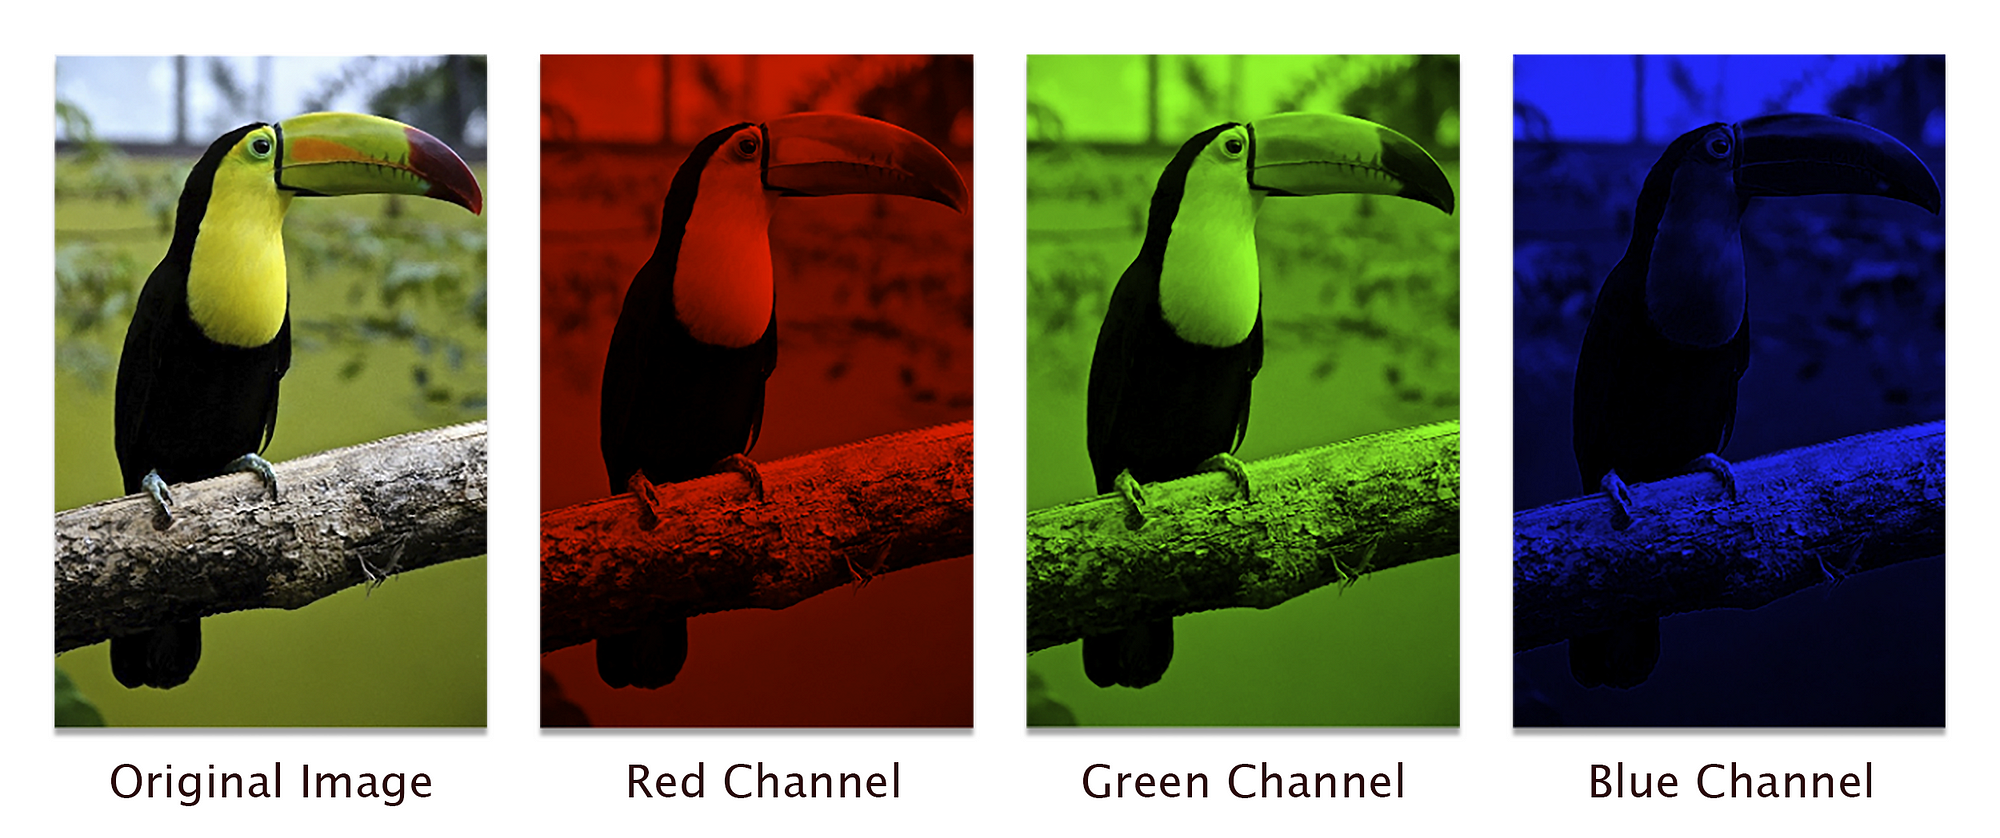
\includegraphics[width=0.7\textwidth]{fig/RGB鸟}
    \end{minipage}
    \hspace{0.2cm}
    \begin{minipage}[H]{0.4\textwidth}
        \centering
        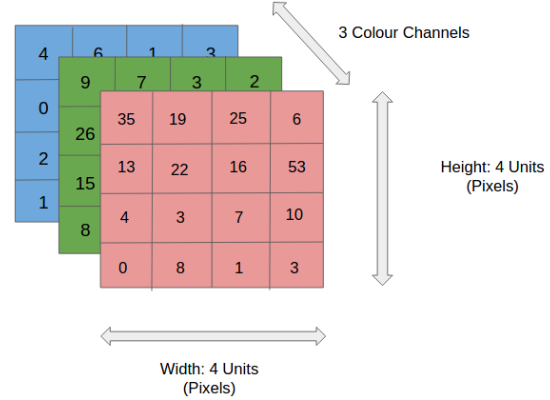
\includegraphics[width=0.7\textwidth]{fig/三通道原始矩阵}
    \end{minipage}
\end{figure}
卷积层的输入通常表示为：
\begin{itemize}
    \item 通道后置表示：$N \times H \times W \times C$；
    \item 通道前置表示：$N \times C \times H \times W$（如 PyTorch）.
\end{itemize}
其中$N$为批量大小，$H$为高度，$W$为宽度，$C$为通道数.
\end{frame}
\subsection{卷积层}
\begin{frame}\frametitle{卷积层}
\begin{mydefinition}[卷积核]
    卷积核是一个小的权重张量，其尺寸通常为 $K_h \times K_w \times D$.它通过对输入局部区域的元素进行加权求和，生成输出特征图对应位置的响应值，用于高效提取局部特征.
\end{mydefinition}
\begin{mydefinition}[卷积层]
    卷积层通过滑动卷积核对输入数据进行计算，提取局部特征，并形成特征图作为输出.深度学习框架中通常实现的是互相关运算，但习惯上仍称为卷积.
\end{mydefinition}
    假设某一卷积层包含 $M$ 个独立卷积核，其中
    \begin{itemize}
        \item 第 $k$ 个卷积核为$\symbf{W}^{(k)} \in \mathbb{R}^{K_h \times K_w \times D}$，
        \item 输入特征图为$\symbf{X} \in \mathbb{R}^{H \times W \times D}$（$D$ 为输入通道数，即上页的 $C$）.
    \end{itemize}
\begin{itemize}
    \item \textbf{滑动卷积操作}：
卷积核在输入特征图上滑动，与对应的局部区域逐元素相乘，并在空间和通道维度上求和，得到第 $k$ 个输出特征图：
    \[
    c_{i,j}^{(k)} = \sum_{u=1}^{K_h} \sum_{v=1}^{K_w} \sum_{d=1}^{D}
    W_{u,v,d}^{(k)} X_{i+u-1,j+v-1,d}
    \]

    \item \textbf{添加偏置项}：
每个卷积值加上第 $k$ 个卷积核的偏置项 $b^{(k)}$，得到 $\symbf{Z}^{(k)}$：
        \[
        z_{i,j}^{(k)} = c_{i,j}^{(k)} + b^{(k)}
        \]

    \item \textbf{输出特征图}：
矩阵 $\symbf{Z}^{(k)}$ 作为第 $k$ 个卷积子层的输出，同时也是非线性层的输入.
\end{itemize}
\begin{center}
    \animategraphics[controls,width=\textwidth]{3}{fig/GIF/convolution_}{1}{16}
\end{center}
卷积层中除卷积核权重外通常还包含下列参数：
\begin{itemize}
    \item padding：填充圈数
\begin{figure}[H]
    \centering
    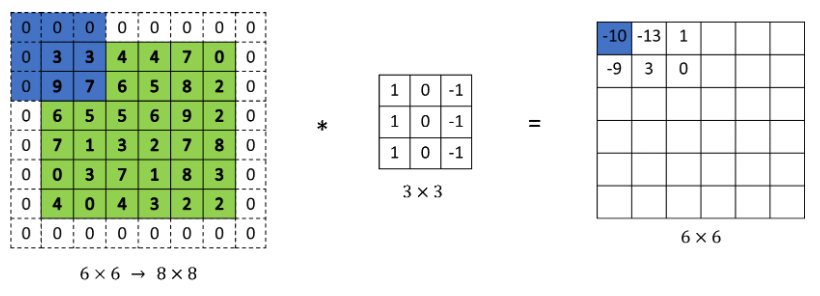
\includegraphics[width=0.6\textwidth]{fig/padding}
\end{figure}
    \item dilation：卷积核膨胀因子
\begin{figure}[H]
    \centering
    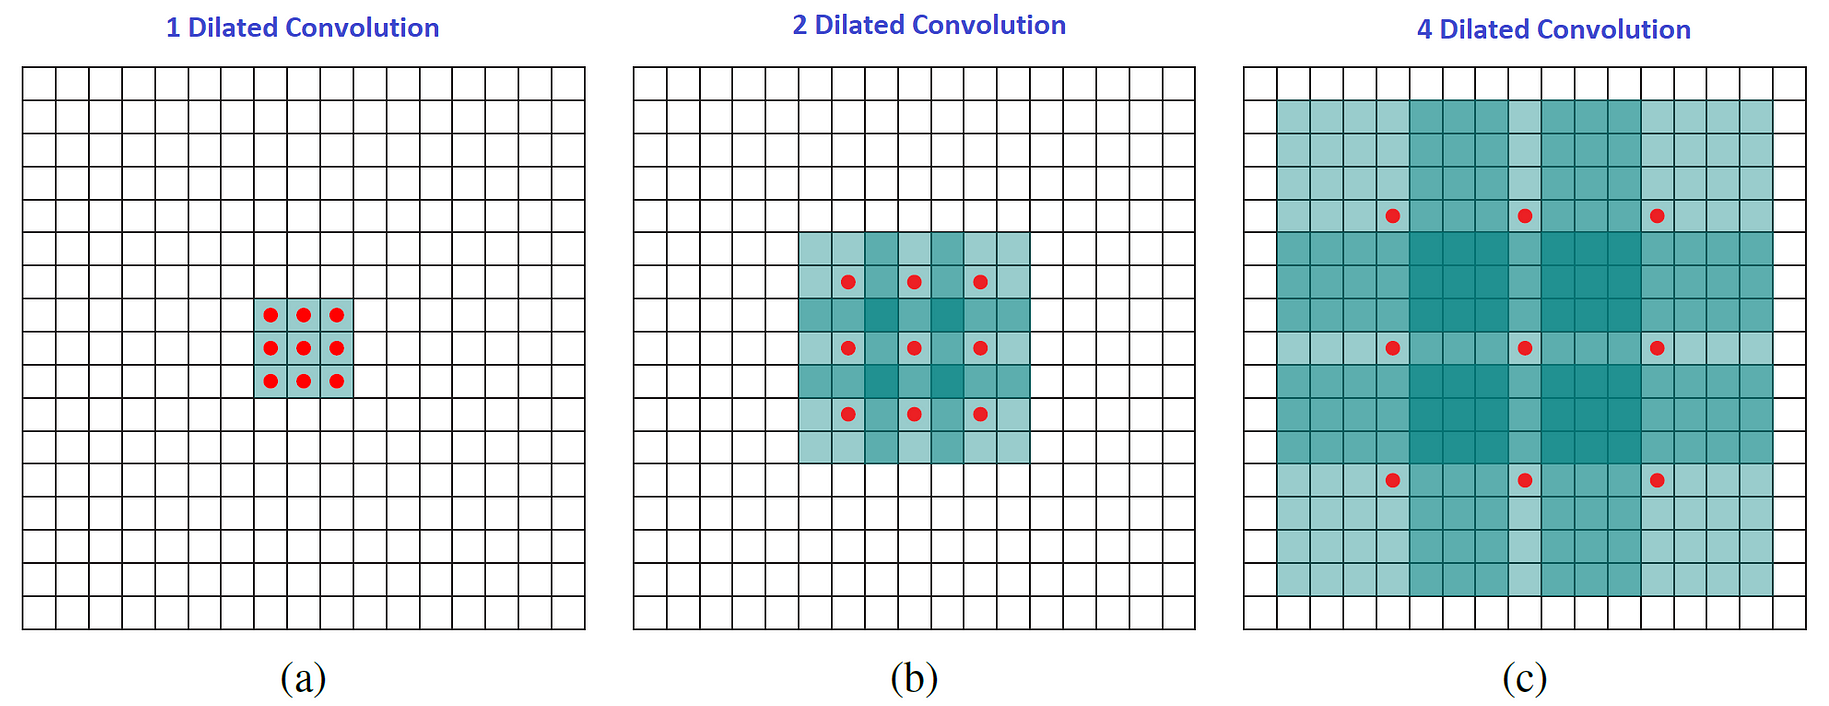
\includegraphics[width=0.6\textwidth]{fig/dilation}
\end{figure}
    \item kernel size：卷积核大小
    \item stride：步长
\begin{figure}[H]
    \centering
    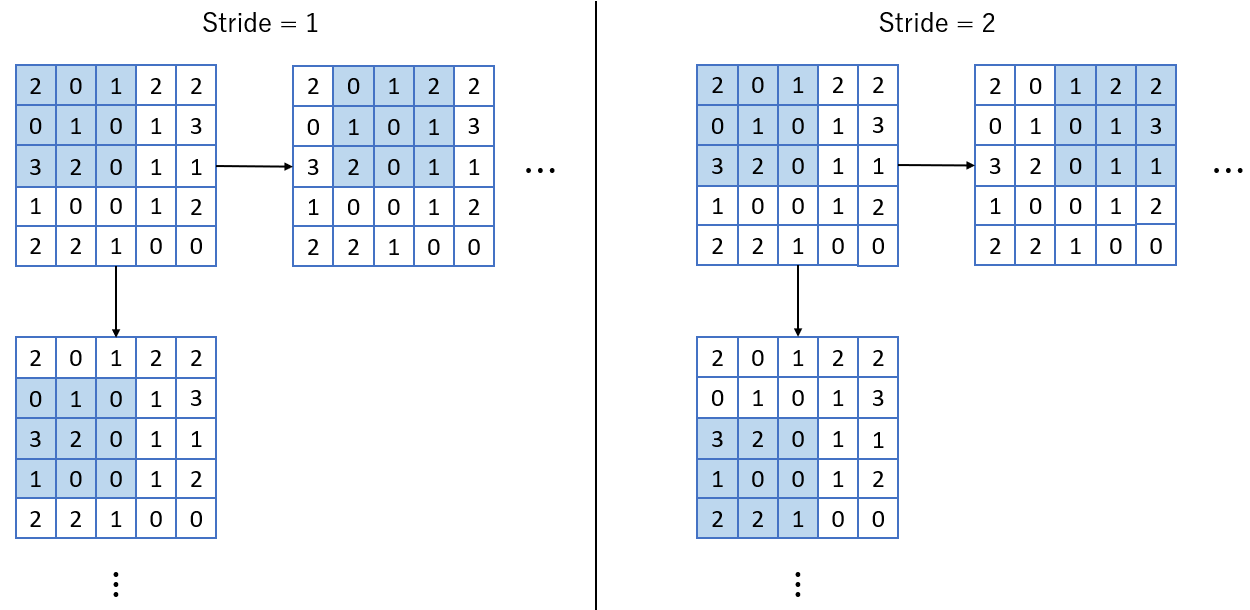
\includegraphics[width=0.85\textwidth]{fig/strides}
\end{figure}
\end{itemize}
通常选择
\begin{itemize}
            \item kernel size $=3\times 3$，padding $=1$，stride $=1$，dilation $=1$.
\end{itemize}
\newpage
\begin{mytheorem}[卷积层特征图尺寸公式]
    每个卷积核生成一个特征图，输出矩阵由全部 $M$ 个卷积核生成的特征图按深度方向拼接而成，其形状为
    $(H_{\text{out}}, W_{\text{out}}, M)$，其中：
        \begin{gather*}
        H_{\text{out}} = \left\lfloor\frac{H_{\text{in}} + 2p_h - d_h(K_h - 1) - 1}{s_h} + 1\right\rfloor
        \end{gather*}
        其中 $p,d,s$ 分别为对应方向的 padding、dilation 与 stride.
\end{mytheorem}
\begin{figure}[H]
    \centering
    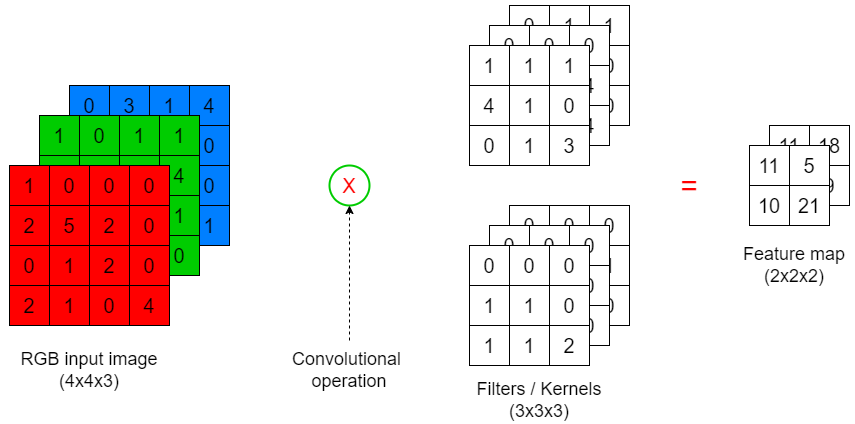
\includegraphics[width=\textwidth,height= 0.4\textheight]{fig/多通道双核CNN}
\end{figure}
\end{frame}

\subsection{非线性层}
\begin{frame}\frametitle{非线性层}
\begin{mydefinition}[非线性层]
    非线性层对特征图中的每个元素逐点应用激活函数 $\phi$：
    \[
    a_{i,j}^{(k)} = \phi(z_{i,j}^{(k)})
    \]
\end{mydefinition}
\begin{minipage}{\textwidth}
    \centering
    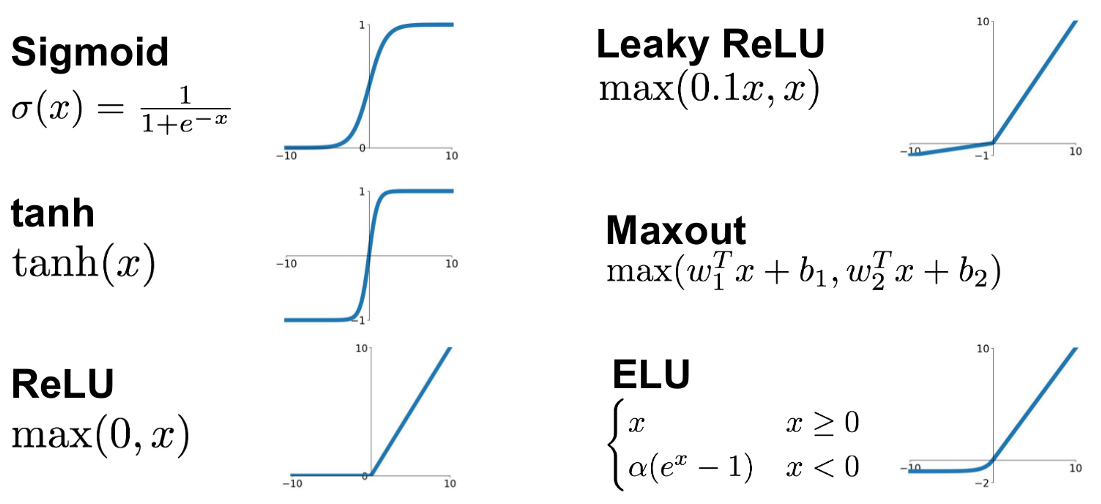
\includegraphics[width=0.4\textwidth]{fig/activation_function}
    \captionof{figure}{常见的非线性激活函数}\label{fig:activation_function}
\end{minipage}
\begin{minipage}{\textwidth}
    通常取：
    \[
    \phi(x) = \mathrm{ReLU}(x) = \max(0,x)
    \]
    \small
    为何必须有非线性层：卷积是线性运算，若无非线性层，任意多层卷积的堆叠仍等价于单个线性变换，网络无法表达复杂的决策边界.选 ReLU 的原因：正区间导数恒为 $1$，深层堆叠时不会像 sigmoid/tanh 那样因饱和而梯度消失；计算仅需一次阈值判断；负半轴置零带来稀疏激活.
\end{minipage}
\end{frame}
\subsection{池化层}
\begin{frame}\frametitle{池化层}
\small
\begin{mydefinition}[池化层]
池化层的主要功能是下采样：通过对特征图的小邻域进行统计处理（如取最大值或均值）来降低空间分辨率，减少后续层的参数量与计算量，从而提高计算效率并增强模型对小幅位移的鲁棒性.
\end{mydefinition}
\textbf{以最大池化为例}：假设池化窗口大小为 $2 \times 2$、步长为 $2$，则第 $k$ 个特征图的池化输出为
\[
    m_{i,j}^{(k)}=\max\left(a_{2i-1,2j-1}^{(k)},a_{2i-1,2j}^{(k)},a_{2i,2j-1}^{(k)},a_{2i,2j}^{(k)}\right)
\]
假设原始输入为 $4 \times 4$ 矩阵：
$\begin{pmatrix}
x_{11} & x_{12} & x_{13} & x_{14} \\
x_{21} & x_{22} & x_{23} & x_{24} \\
x_{31} & x_{32} & x_{33} & x_{34} \\
x_{41} & x_{42} & x_{43} & x_{44} \\
\end{pmatrix}$
则经过最大池化后的输出为：
\[
\begin{pmatrix}
    \max(x_{11},x_{12},x_{21},x_{22}) & \max(x_{13},x_{14},x_{23},x_{24}) \\
    \max(x_{31},x_{32},x_{41},x_{42}) & \max(x_{33},x_{34},x_{43},x_{44}) \\
\end{pmatrix}
\]
\end{frame}
\subsection{全连接层}
\begin{frame}\frametitle{全连接层}
\begin{mydefinition}[全连接层]
全连接层位于卷积神经网络的末端，通过整合卷积层和池化层提取的高维特征，将其映射为最终的分类或回归结果.
\end{mydefinition}
\begin{figure}[H]
\centering
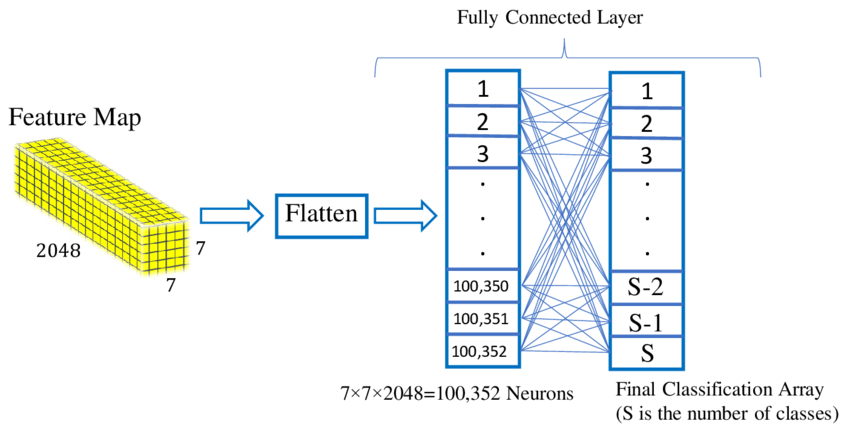
\includegraphics[width=0.85\textwidth]{fig/Classification-with-Flatten-and-Fully-Connected-layers}
\end{figure}
\end{frame}
%-- 完整的CNN网络结构 ------------------------------------------------------------------
\subsection{完整结构示例}
\begin{frame}\frametitle{卷积神经网络的完整结构示例}
\begin{figure}[H]
\centering
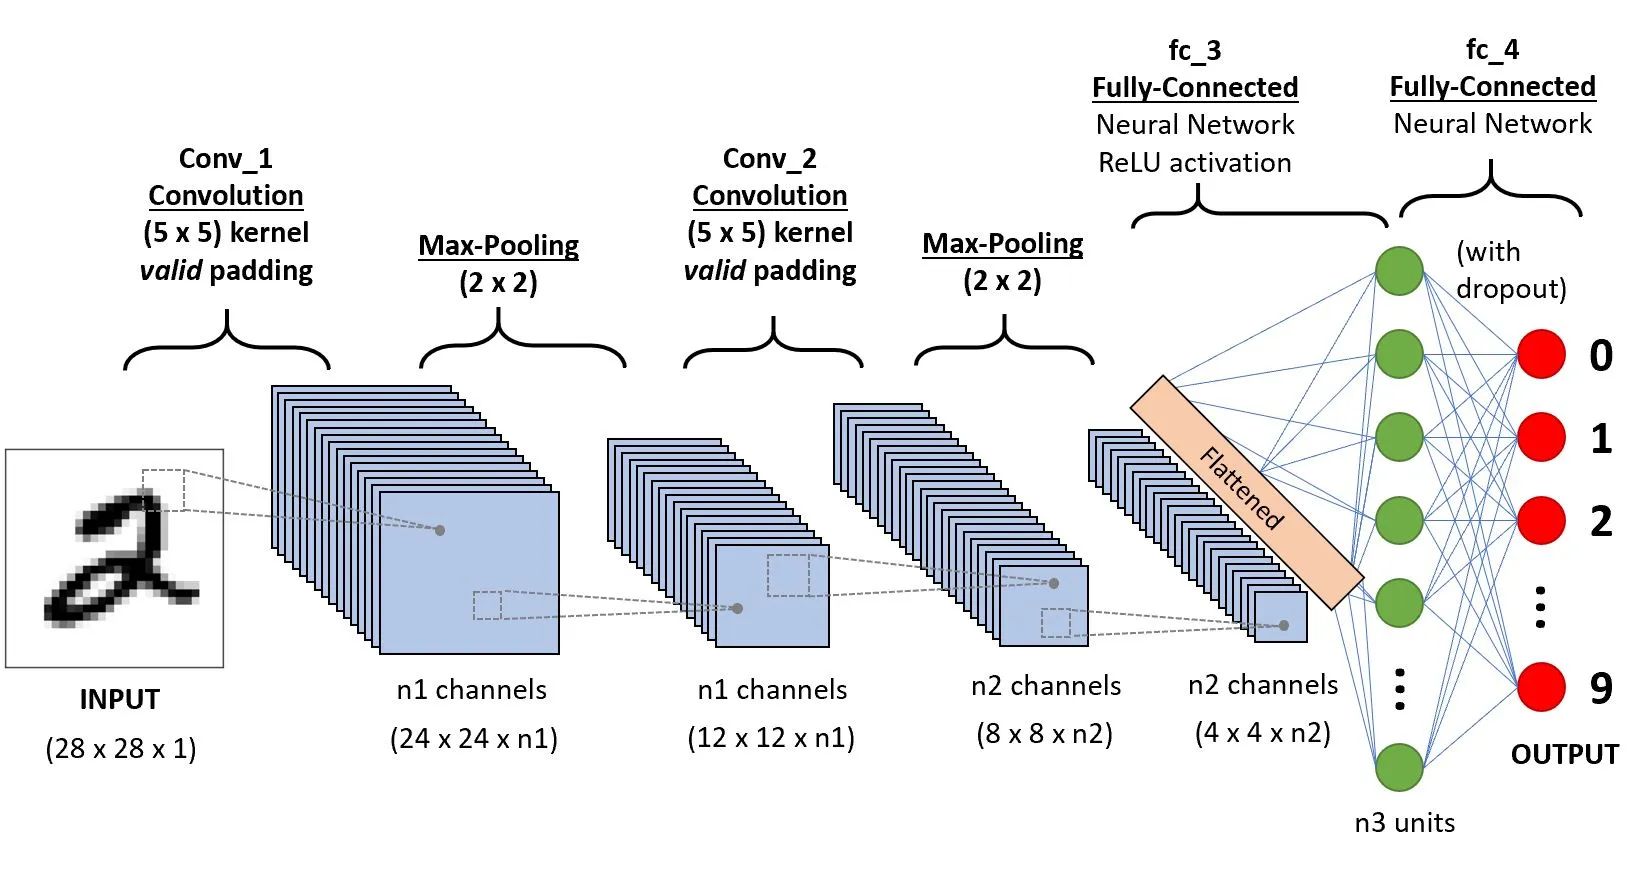
\includegraphics[width=\textwidth]{fig/img_3}
\caption{卷积神经网络的完整结构示例}\label{fig:fully_connected_layer}
\end{figure}
\end{frame}
\section{Transformer简要原理}
\subsection{注意力机制}
\begin{frame}\frametitle{注意力机制}
    \begin{columns}
         \begin{column}{0.5\textwidth}
        \begin{figure}
            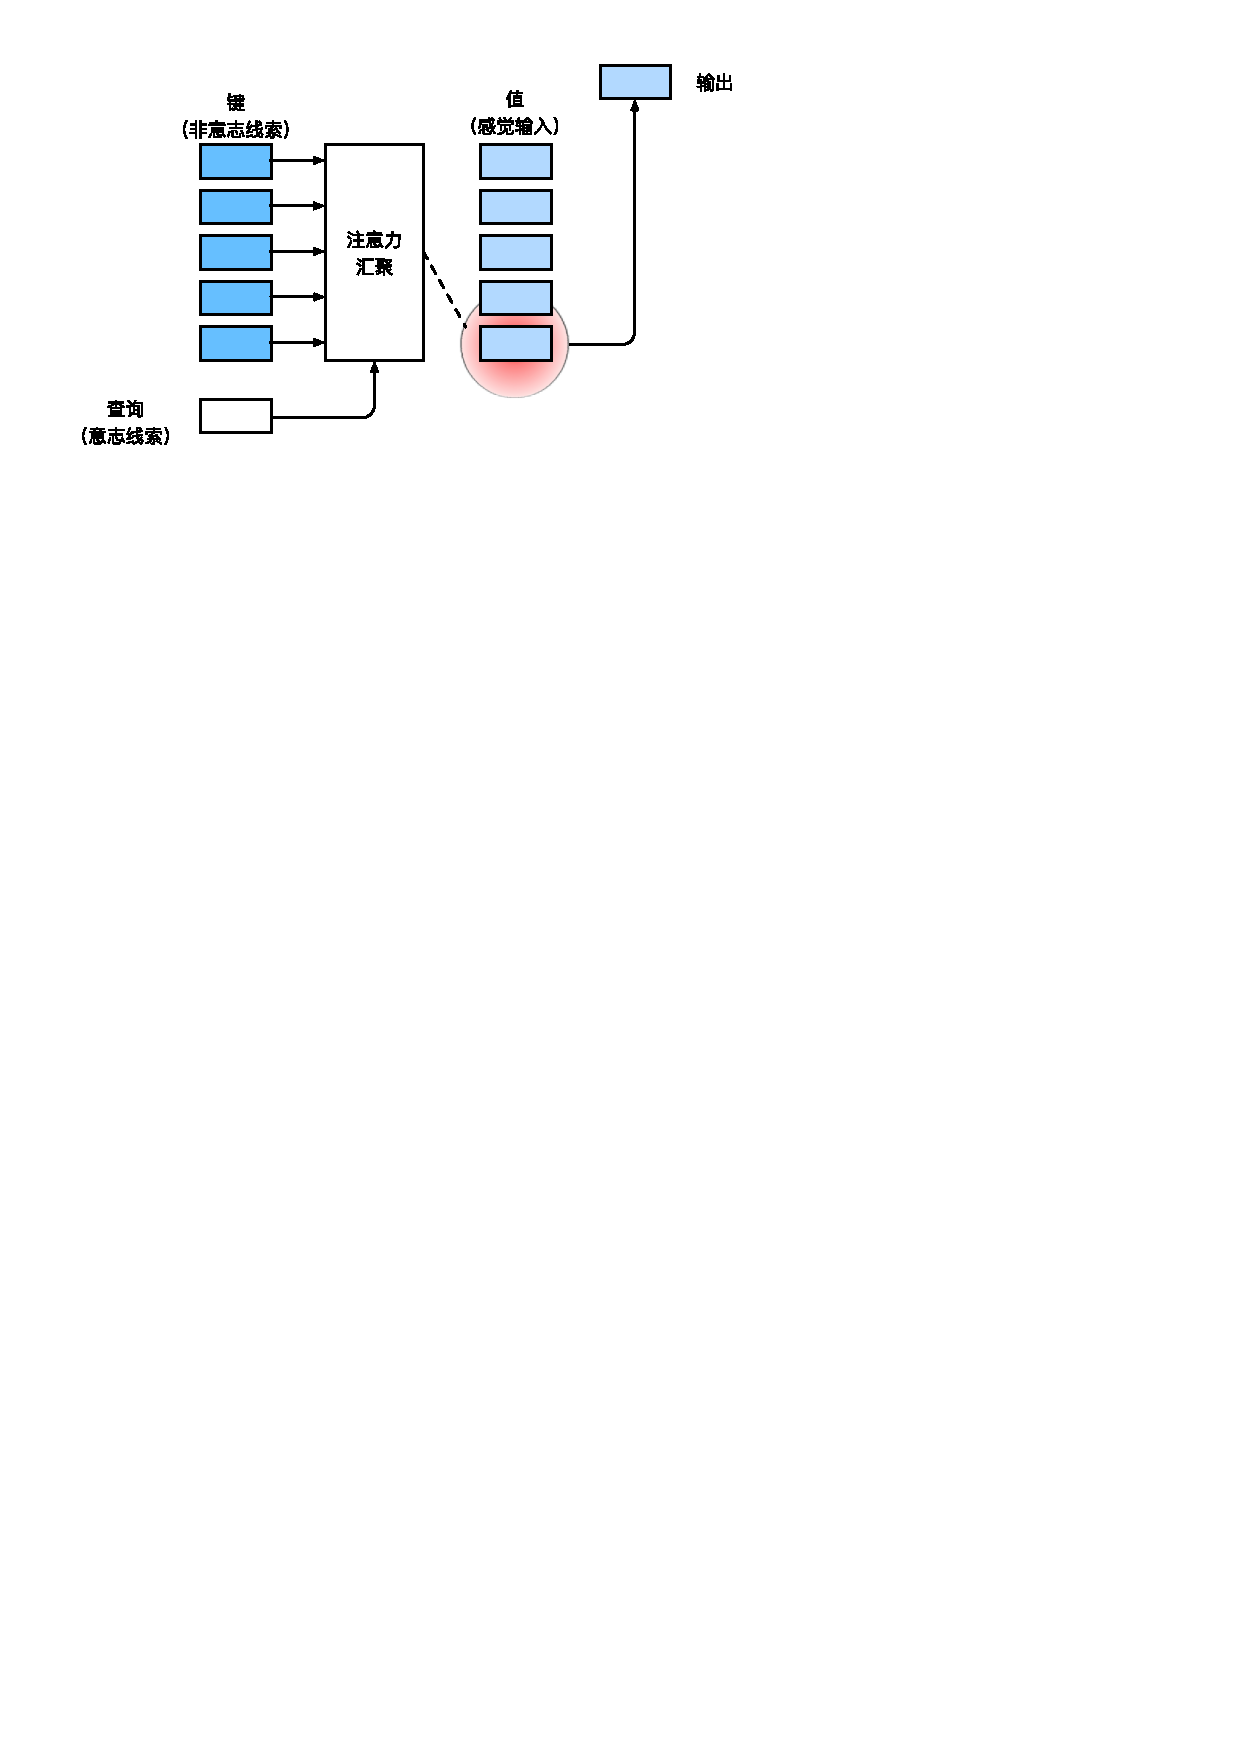
\includegraphics[width=\textwidth, height=0.32\textheight]{figure/qkv}
            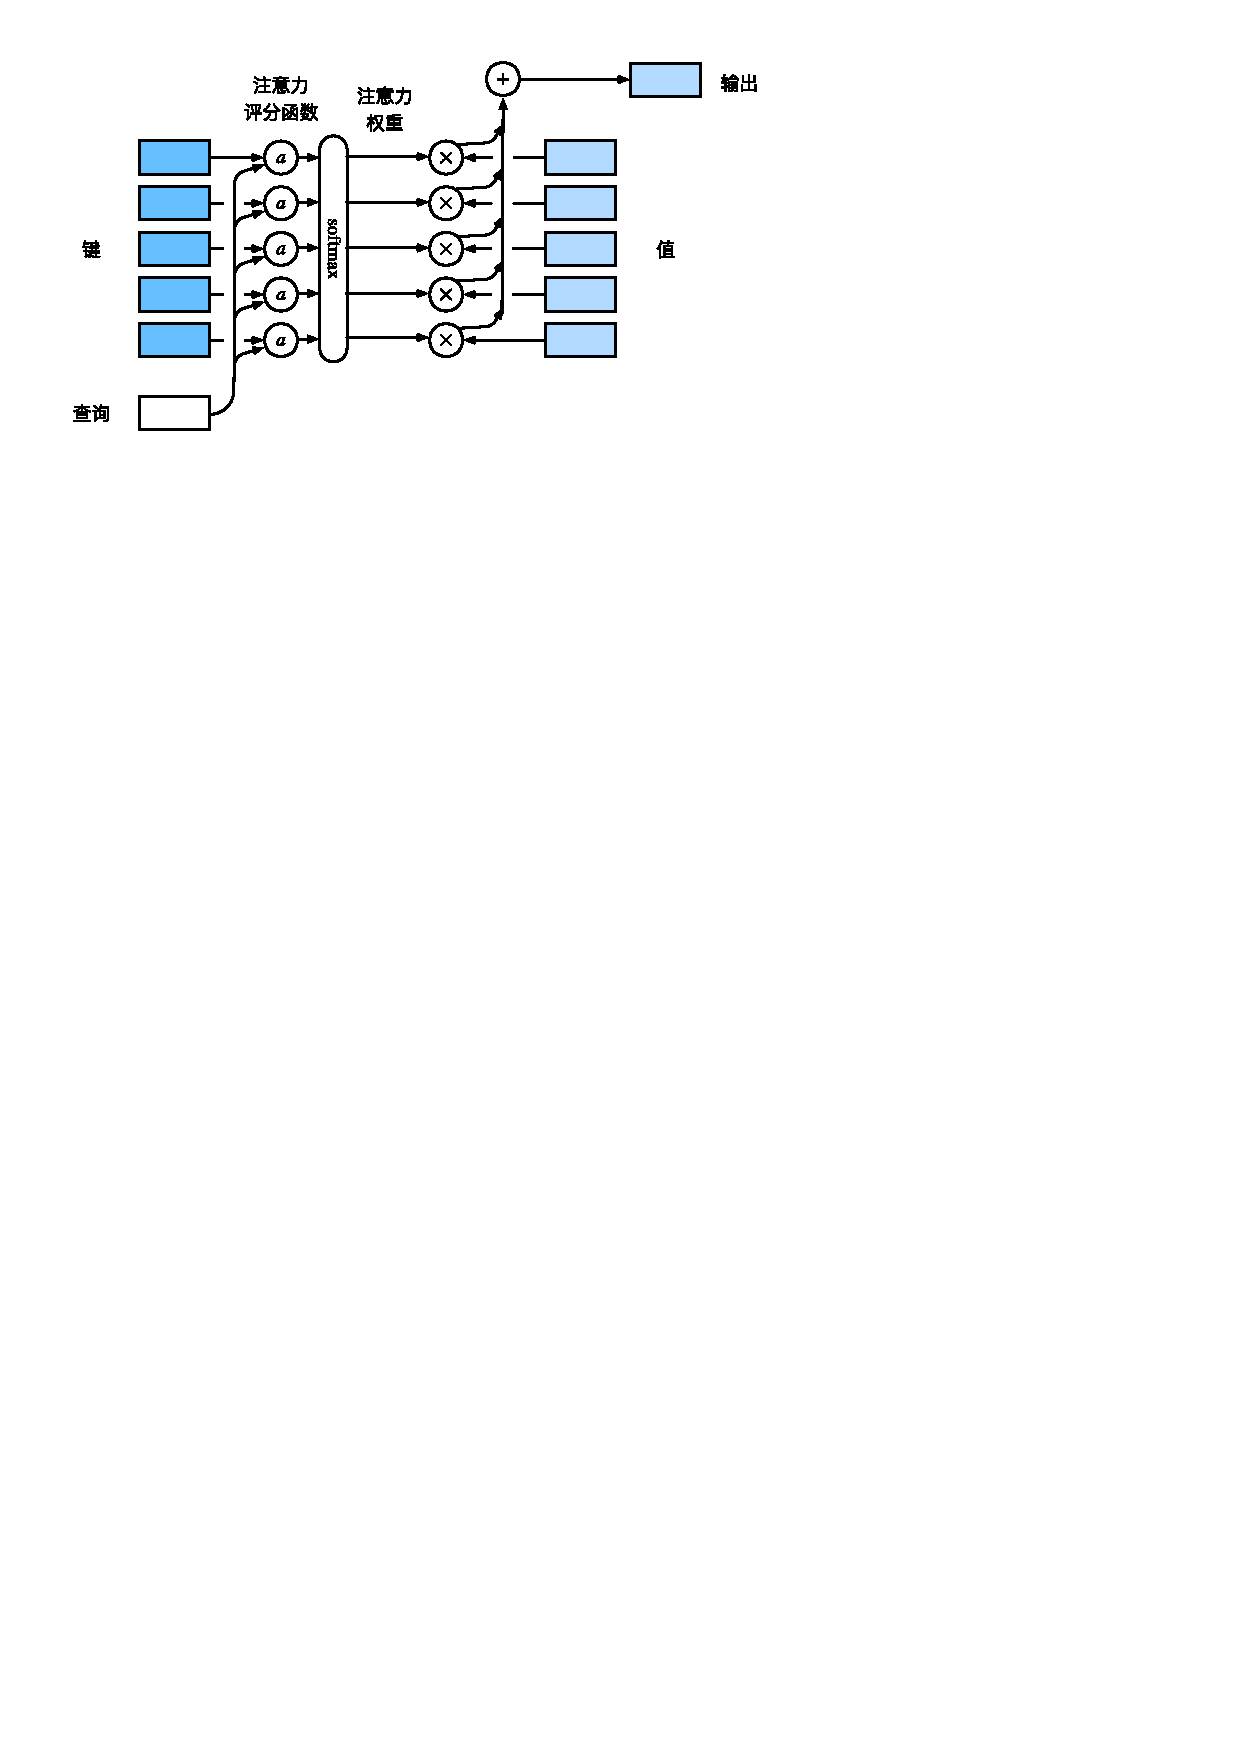
\includegraphics[width=\textwidth, height=0.32\textheight]{figure/attention-output}
            \caption{注意力的查询—键—值机制与汇聚输出}
        \end{figure}
        \end{column}
        \begin{column}{0.5\textwidth}
            \footnotesize
            \centering
            \begin{itemize}
                \item 查询（$\symbf{q} \in \mathbb{R}^{d_q}$）：自主提示——当前“想找什么”
                \item 键值对 $(\symbf{k}_i, \symbf{v}_i),\ i=1,2,\ldots,n$
                \begin{itemize}
                \item 键（$\symbf{k}_i \in \mathbb{R}^{d_k}$）：非自主提示——各条信息的“索引”
                \item 值（$\symbf{v}_i \in \mathbb{R}^{d_v}$）：感官输入——信息内容本身
                \end{itemize}
            \end{itemize}
            \begin{itemize}
                \item $a(\symbf{q}, \symbf{k}_{i}) \in \mathbb{R}$：注意力评分
                \item $\alpha(\symbf{q}, \symbf{k}_i)$：注意力权重，恒正且 $\sum_{i=1}^{n}\alpha(\symbf{q}, \symbf{k}_i)=1$
                \item $f\left(\symbf{q}, \{(\symbf{k}_i, \symbf{v}_i)\}_{i=1}^{n}\right) \in \mathbb{R}^{d_v}$：注意力汇聚
            \end{itemize}
            \begin{align*}
                \alpha(\symbf{q}, \symbf{k}_i)
                &= \frac{\exp(a(\symbf{q}, \symbf{k}_i))}{\sum_{j=1}^n \exp(a(\symbf{q}, \symbf{k}_j))}\\
                f\left(\symbf{q}, \{(\symbf{k}_i, \symbf{v}_i)\}_{i=1}^{n}\right)
                &= \sum_{i=1}^n \alpha(\symbf{q}, \symbf{k}_i) \symbf{v}_i
            \end{align*}
            \end{column}
     \end{columns}
直观上，注意力是一次\textbf{可微的“软查表”}：硬查表按键精确匹配、取出一条值；注意力按查询与各键的相似度，对全部值做凸组合——相似度越高的条目贡献越大，且整个过程可对相似度求导，从而能端到端学习“该看哪里”.
\begin{itemize}
    \item 两种流行的注意力评分函数：
    \begin{itemize}
    \item 加性注意力：即使查询 $\symbf{q} \in \mathbb{R}^{d_q}$ 与键 $\symbf{k} \in \mathbb{R}^{d_k}$ 的维度不同（$d_q\neq d_k$）也适用：
    \begin{equation*}
a(\symbf{q}, \symbf{k})=\symbf{w}_a^{\top} \tanh \left(\symbf{W}_q \symbf{q}+\symbf{W}_k \symbf{k}\right) \in \mathbb{R}
    \end{equation*}
    其中 $\symbf{W}_q\in\mathbb{R}^{d_h\times d_q}$、$\symbf{W}_k\in\mathbb{R}^{d_h\times d_k}$、$\symbf{w}_a\in\mathbb{R}^{d_h}$ 均为可学习参数，$d_h$ 为隐藏单元数.
    \item 缩放点积注意力：要求查询与键同维（$d_q=d_k$）：
    \begin{columns}
        \begin{column}{0.2\textwidth}
            \begin{figure}[H]
                \raggedleft
                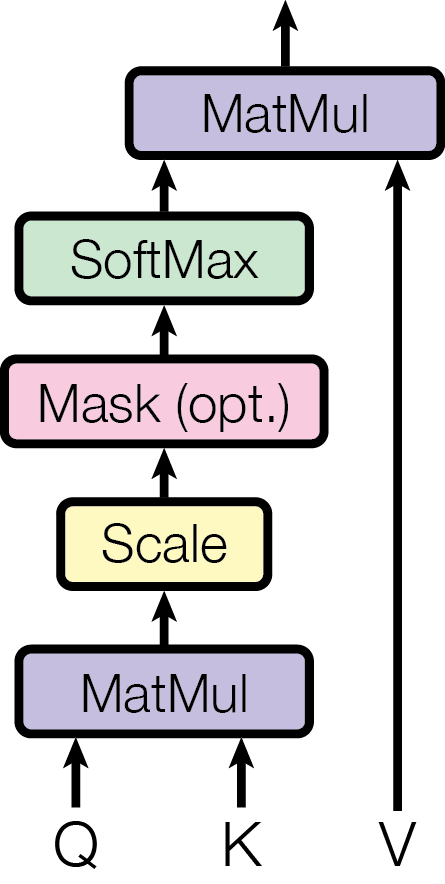
\includegraphics[width=0.4\textwidth, height=0.2\textheight]{figure/ModalNet-19}
            \end{figure}
        \end{column}
        \begin{column}{0.8\textwidth}
        \small
        \begin{align*}
a(\symbf{q}, \symbf{k})
&= \frac{\symbf{q}^{\top} \symbf{k}}{\sqrt{d_k}} \in \mathbb{R}\\
\mathrm{Attention}(\symbf{Q}, \symbf{K}, \symbf{V})
&= \mathrm{softmax}\left(
\frac{\symbf{Q}\symbf{K}^{\top}}{\sqrt{d_k}}
\right)\symbf{V}
        \end{align*}
        \end{column}
    \end{columns}
    矩阵形式中，$m$ 个查询与 $n$ 个键、值分别按行堆叠为 $\symbf{Q}\in\mathbb{R}^{m\times d_k}$、$\symbf{K}\in\mathbb{R}^{n\times d_k}$、$\symbf{V}\in\mathbb{R}^{n\times d_v}$，故 $\symbf{Q}\symbf{K}^{\top}\in\mathbb{R}^{m\times n}$ 的 $(i,j)$ 元为 $\symbf{q}_i^{\top}\symbf{k}_j$，除以 $\sqrt{d_k}$ 后即评分 $a(\symbf{q}_i,\symbf{k}_j)$；softmax 对缩放后的评分矩阵\textbf{逐行}作用.缩放因子$\sqrt{d_k}$的作用：若$\symbf{q},\symbf{k}$的各分量相互独立、均值为$0$、方差为$1$，则$\symbf{q}^{\top}\symbf{k}$的方差为$d_k$；除以$\sqrt{d_k}$使评分方差保持为$1$，避免内积随维度增大而过大、softmax进入饱和区导致梯度消失.
    \end{itemize}
    \item 掩蔽softmax：先将无效位置的注意力评分置为$-\infty$，再经 softmax 使其权重为$0$：
    \begin{figure}[H]
        \centering
        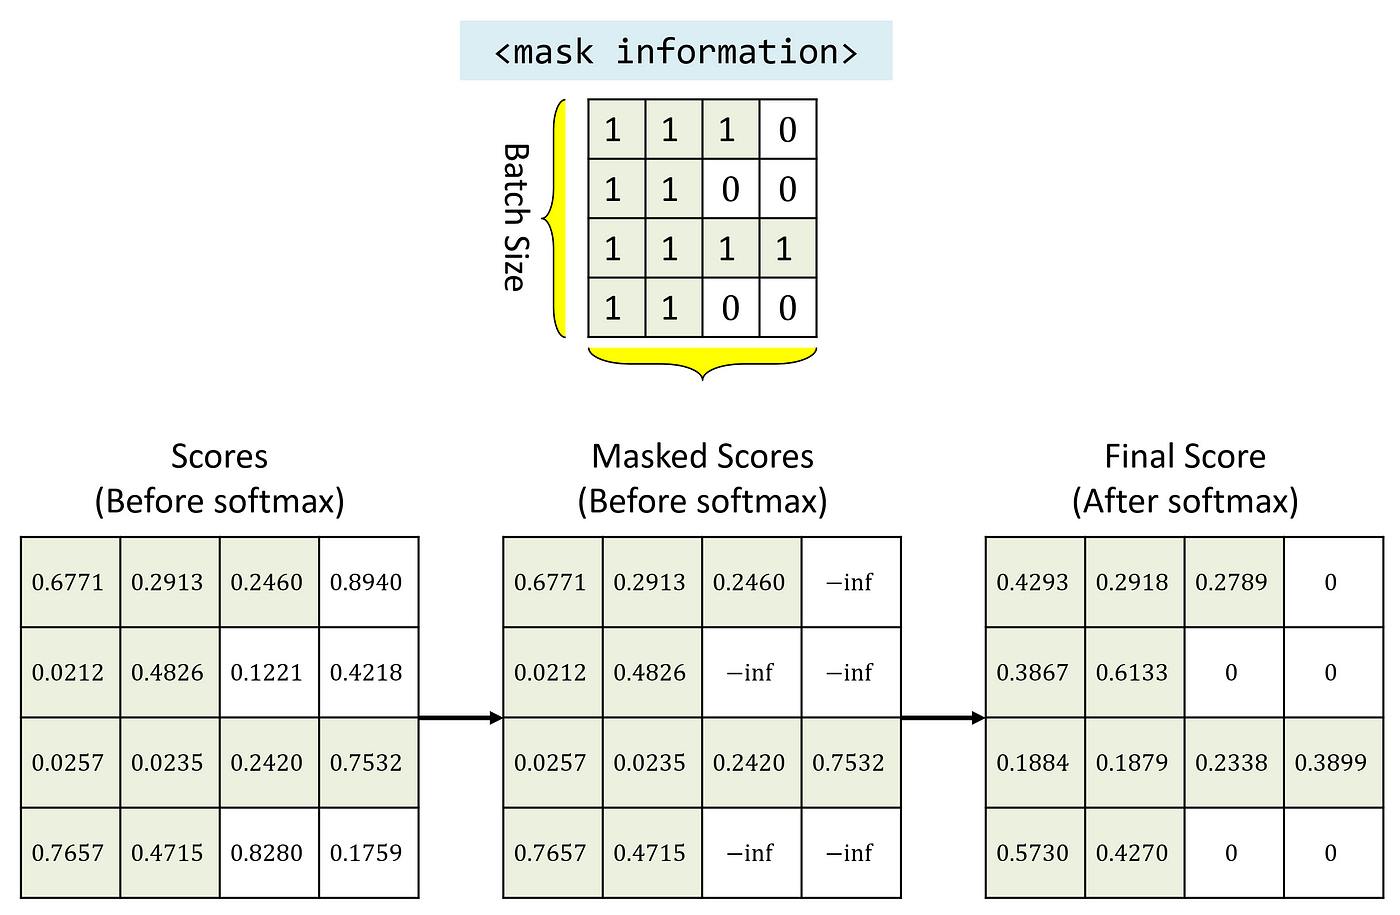
\includegraphics[width=0.8\textwidth, height=0.32\textheight]{figure/masked-softmax}
        \caption{掩蔽 softmax：屏蔽无效位置后再归一化}
    \end{figure}
    \item 多头注意力机制：通过多个注意力头并行计算，使模型能够在不同的表示子空间中关注来自不同位置的信息.单头注意力对每个位置只产生一组凸组合权重，难以同时表达多种关注模式（如句法邻近与语义呼应）；多头将 $d_{\mathrm{model}}$ 拆分为 $h$ 个低维子空间（每头 $d_k=d_{\mathrm{model}}/h$）各自学习一种模式后在列方向上拼接融合——类比 CNN 中并行的多组卷积核.
    \vspace{0.5em}
    \begin{columns}
        \begin{column}{0.25\textwidth}
            \begin{figure}[H]
                \centering
                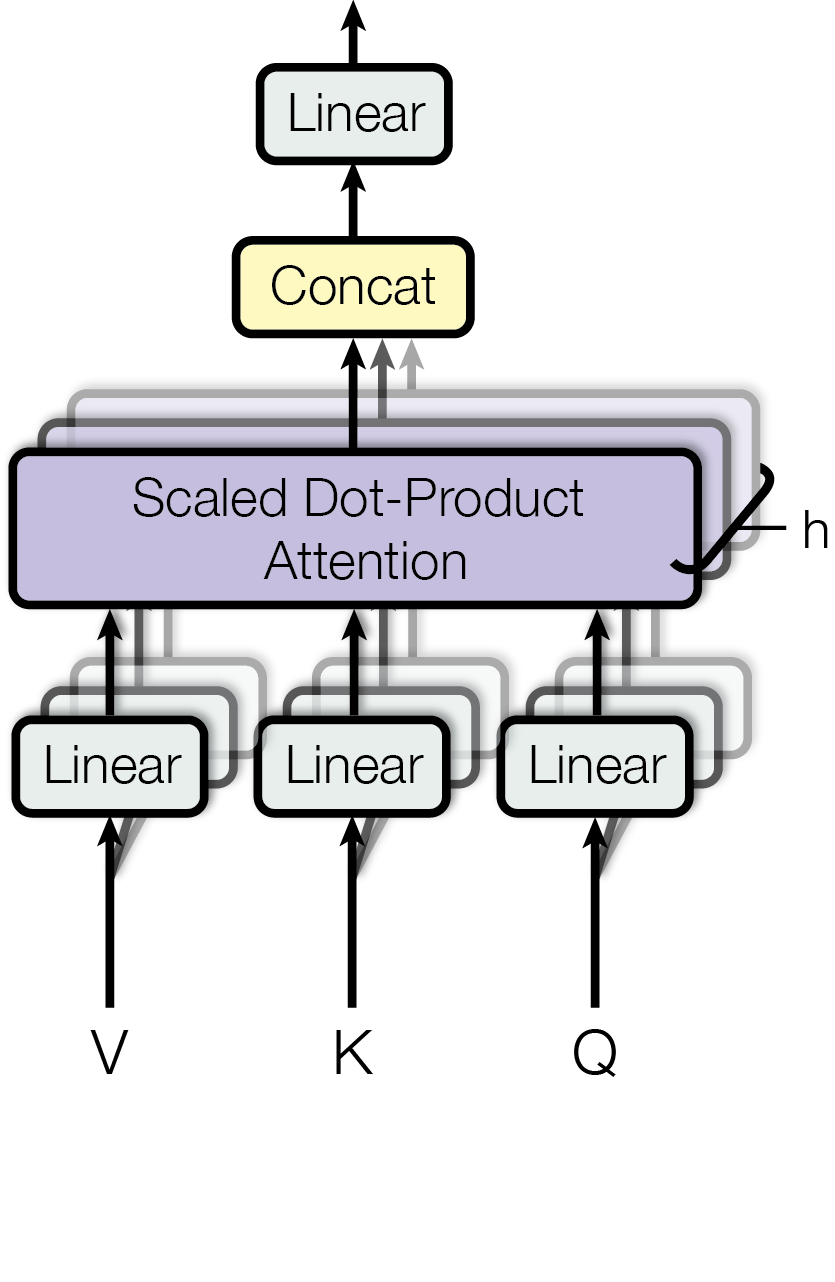
\includegraphics[width=0.8\textwidth]{figure/ModalNet-20}
            \end{figure}
        \end{column}
        \begin{column}{0.2\textwidth}
            \begin{figure}[H]
                \centering
        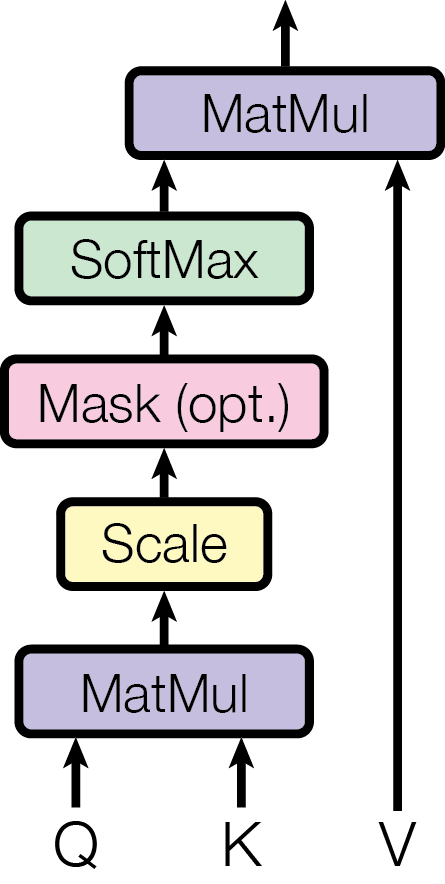
\includegraphics[width=0.4\textwidth]{figure/ModalNet-19}
            \end{figure}
        \end{column}
        \begin{column}{0.5\textwidth}
        \footnotesize
        \begin{align*}
            &\mathrm{MultiHead}(\symbf{Q}, \symbf{K}, \symbf{V}) =
            \mathrm{Concat}(\symbf{h}_1,\ldots,\symbf{h}_h)\symbf{W}^{O}\\
            &\symbf{h}_{i} = \mathrm{Attention}\left(\symbf{Q}\symbf{W}_{i}^{Q}, \symbf{K}\symbf{W}_{i}^{K}, \symbf{V}\symbf{W}_{i}^{V}\right)
        \end{align*}
         其中 $\symbf{h}_i$ 为第 $i$ 个头的输出；此处 $\symbf{Q},\symbf{K},\symbf{V}$ 为未投影的输入表示（列宽 $d_{\mathrm{model}}$）；$\symbf{W}_{i}^{Q},\symbf{W}_{i}^{K}\in\mathbb{R}^{d_{\mathrm{model}}\times d_k}$、$\symbf{W}_{i}^{V}\in\mathbb{R}^{d_{\mathrm{model}}\times d_v}$、$\symbf{W}^{O}\in\mathbb{R}^{h d_v\times d_{\mathrm{model}}}$ 均为可学习参数.
        \end{column}
    \end{columns}
    \newpage
    维度小结：为何处处取 $d_{\mathrm{model}}$?
    \footnotesize
    \begin{itemize}
        \item \textbf{注意力运算的硬约束}（只锁定投影\emph{后}的内部维度，$d_k,d_v$ 原则上可自由取）：
        \begin{center}
            \small
            \renewcommand{\arraystretch}{1.1}
            \begin{tabular}{@{}lll@{}}
                \toprule
                运算 & 维度\textbf{须相同} & 维度\textbf{可不同}\\
                \midrule
                $\symbf{Q}\symbf{K}^{\top}$ & \textbf{列}：$d_k$（否则点积无定义） & \textbf{行}：查询数 $n_q$、键值数 $n_k$\\
                $\mathrm{softmax}(\cdot)\,\symbf{V}$ & \textbf{行}：$n_k$（键与值唯一配对） & \textbf{列}：键维 $d_k$、值维 $d_v$\\
                \bottomrule
            \end{tabular}
        \end{center}
        \item \textbf{为何统一取 $d_{\mathrm{model}}$}（作用于\emph{未投影}输入与多头\emph{输出}的\textbf{架构}约束）：$d_{\mathrm{model}}$ 是贯穿各层的\textbf{残差流宽度}——子层须\emph{入}、\emph{出}同宽，残差连接 $\symbf{x}+\mathrm{Sublayer}(\symbf{x})$ 方能逐元素相加、各层方可同构堆叠。故投影矩阵 $\symbf{W}^{Q}_i,\symbf{W}^{K}_i,\symbf{W}^{V}_i$ 的输入侧均为 $d_{\mathrm{model}}$，$\symbf{W}^{O}$ 再把拼接所得的 $h d_v$ 映回 $d_{\mathrm{model}}$；自注意力中 $\symbf{Q},\symbf{K},\symbf{V}$ 同源于 $\symbf{X}$，未投影列宽自然皆为 $d_{\mathrm{model}}$。
        \item \textbf{内部维度的惯例}：取 $d_k=d_v=d_{\mathrm{model}}/h$，使 $h$ 个头的总开销 $\approx$ 单个全维头，且 $\mathrm{Concat}$ 后 $h d_v=d_{\mathrm{model}}$ 恰好还原。
    \end{itemize}
    \newpage
    \item 自注意力：查询、键和值来自同一组输入 $\symbf{X}\in\mathbb{R}^{n\times d_{\mathrm{model}}}$（$n$ 个位置的表示按行堆叠）：
    \begin{columns}
        \begin{column}{0.4\textwidth}
            \begin{figure}[H]
                \centering
                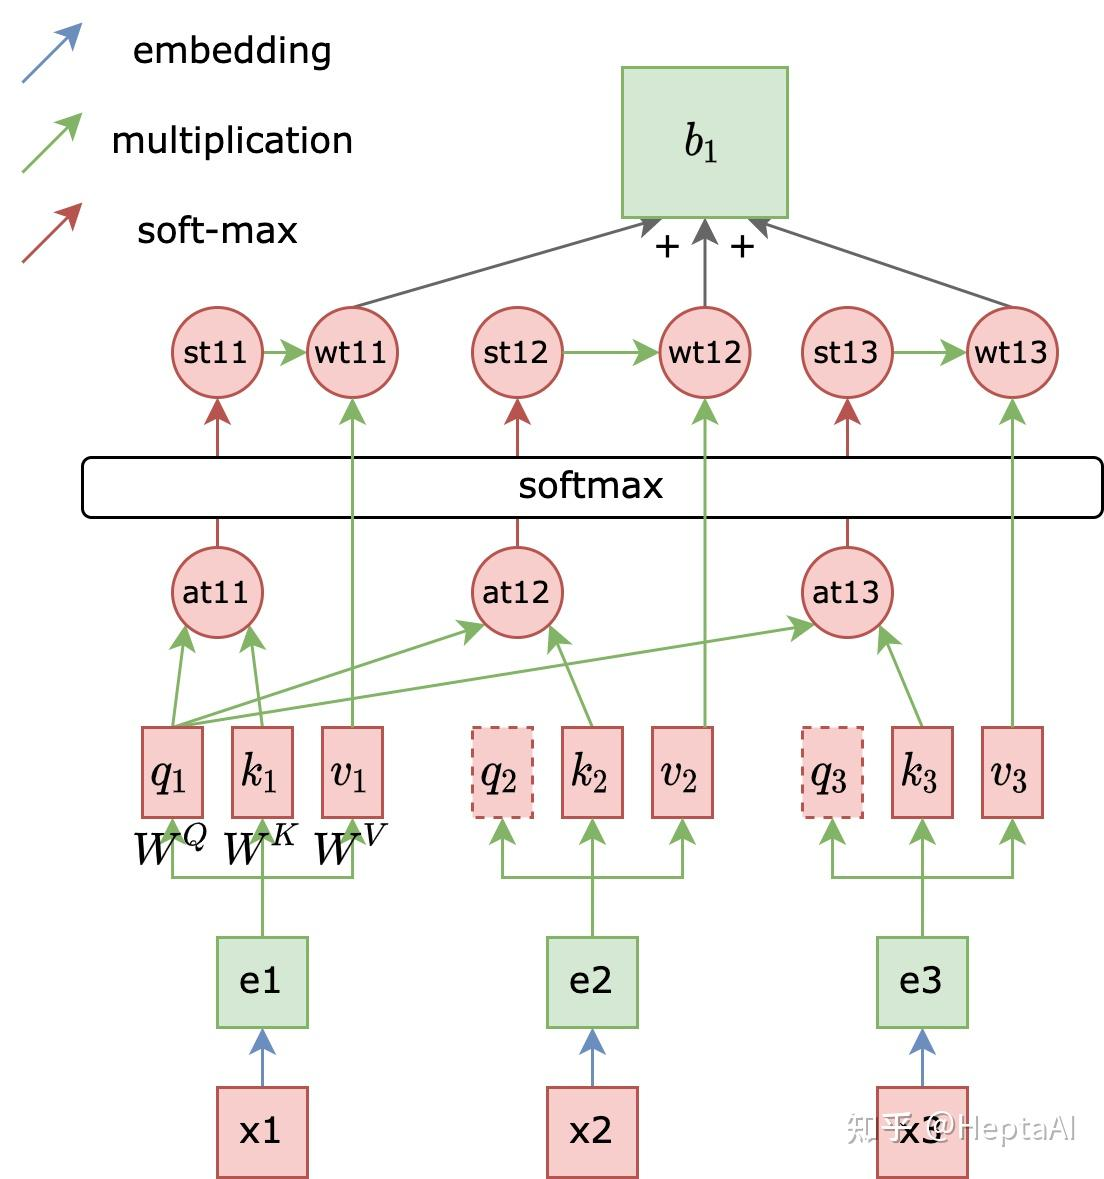
\includegraphics[width=\textwidth]{figure/self-attention}
                \caption{Q、K、V 同源于输入 X}
            \end{figure}
        \end{column}
        \begin{column}{0.6\textwidth}
    \footnotesize
    \begin{align*}
        &\symbf{Q}=\symbf{X}\symbf{W}^Q,\\
        &\symbf{K}=\symbf{X}\symbf{W}^K,\\
        &\symbf{V}=\symbf{X}\symbf{W}^V
    \end{align*}
    其中 $\symbf{W}^{Q},\symbf{W}^{K}\in\mathbb{R}^{d_{\mathrm{model}}\times d_k}$，$\symbf{W}^{V}\in\mathbb{R}^{d_{\mathrm{model}}\times d_v}$.
    
    \begin{equation*}
        \mathrm{Attention}(\symbf{X})=\mathrm{softmax}\!\left(\frac{(\symbf{X}\symbf{W}^{Q})(\symbf{X}\symbf{W}^{K})^{\top}}{\sqrt{d_k}}\right)\symbf{X}\symbf{W}^{V}.
    \end{equation*}
    \end{column}
        \end{columns}
    \newpage
    \item 位置编码：自注意力具有\textbf{置换等变性}——对输入序列做任意置换，输出仅做相同置换，各位置的表示本身不携带任何顺序信息；
    这不像RNN那样通过隐状态的逐步传递天然引入位置信息.为了使模型能够利用文本序列中的位置信息，需在输入嵌入中加入位置编码，用以引入绝对或相对的位置信息，如：
    \begin{align*}
    \mathrm{PE}_{pos,2i}&=\sin\left( pos/10000^{2i/d_{\mathrm{model}}}\right),\\
    \mathrm{PE}_{pos,2i+1}&=\cos\left( pos/10000^{2i/d_{\mathrm{model}}}\right)
    \end{align*}
    其中 $pos$ 为位置索引，$i$ 为维度对索引（$0\le 2i,\,2i+1<d_{\mathrm{model}}$）.
    \begin{figure}[H]
        \centering
        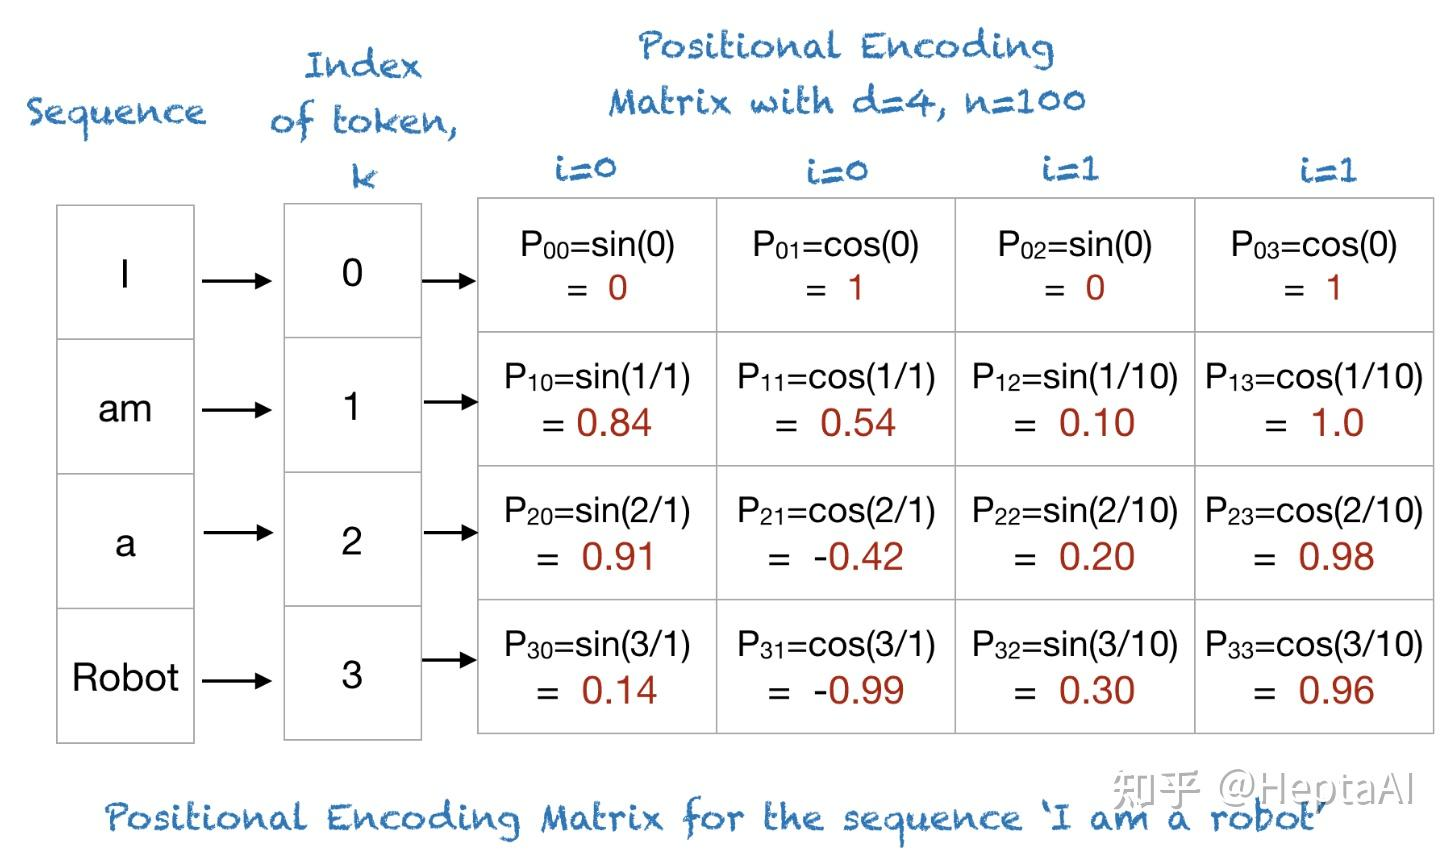
\includegraphics[height=0.5\textheight]{figure/positional-encoding}
    \end{figure}
\end{itemize}
\end{frame}

\subsection{Transformer架构}
\begin{frame}\frametitle{Transformer架构：注意力层}
    \begin{columns}[T]
        \begin{column}{0.4\textwidth}
            \begin{figure}[H]
                \centering
                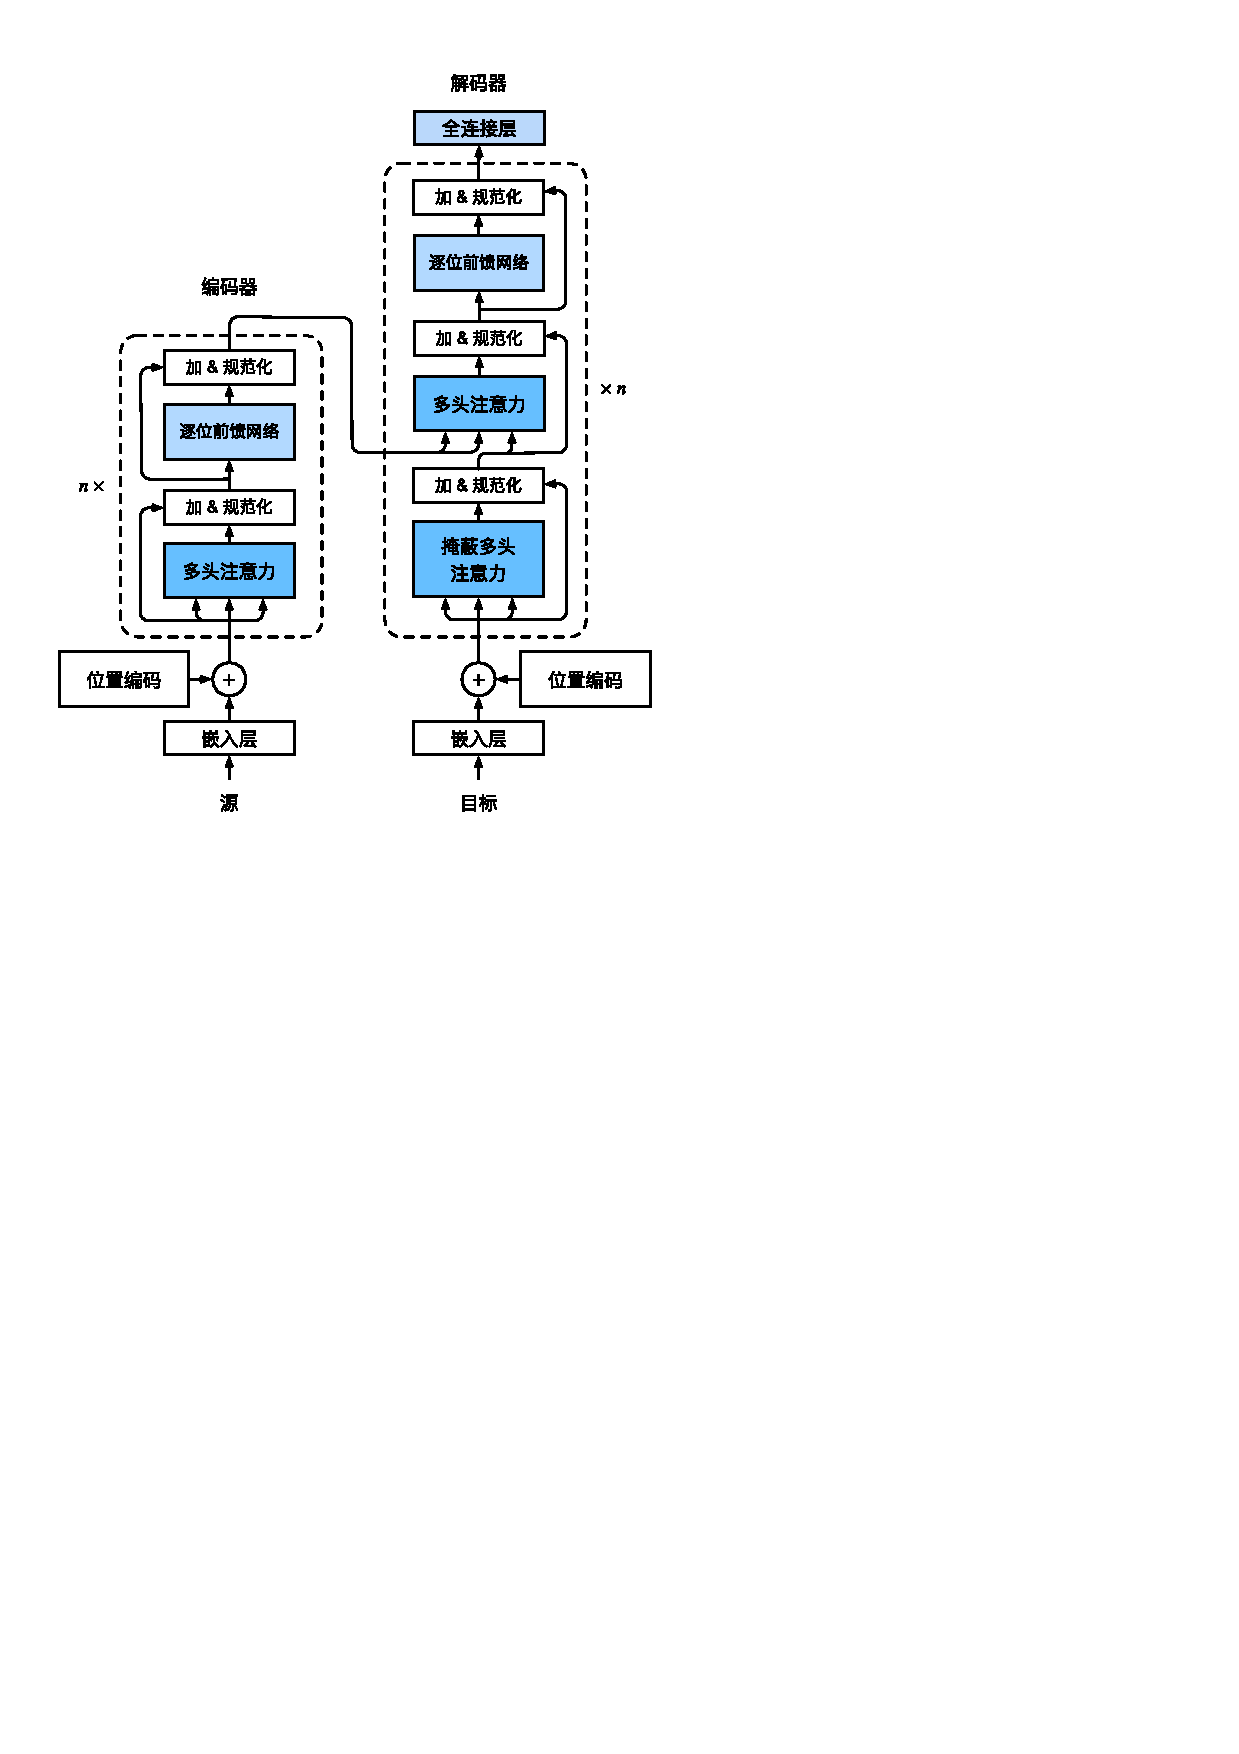
\includegraphics[width=\textwidth, height=0.75\textheight]{figure/transformer}
                \caption{Transformer 整体架构}\label{fig:transformer}
            \end{figure}
        \end{column}
        \begin{column}{0.6\textwidth}
            \footnotesize
            \begin{itemize}
        \item （编码器中）多头自注意力层（Multi-head Self-attention Layer）：
        \begin{enumerate}
            \item 查询、键、值：由前一编码器层输出分别线性投影得到
            \item 编码器中的每个位置都可以关注编码器前一层中的所有位置
        \end{enumerate}
        \item （解码器中）编码器-解码器注意力层（Encoder-Decoder Attention Layer）：
        \begin{enumerate}
            \item 查询：由前一解码器层输出线性投影得到
            \item 键、值：由编码器输出线性投影得到
            \item 解码器中的每个位置都能关注输入序列的所有位置
        \end{enumerate}
        \item （解码器中）掩蔽多头自注意力层（Masked Multi-head Self-attention Layer）：
        \begin{enumerate}
            \item 查询、键、值：由上一解码器层输出分别线性投影得到
            \item 解码器中的每个位置只能关注该位置及其之前的所有位置，以保持自回归性质、防止训练时泄漏未来信息
        \end{enumerate}
                \end{itemize}
        \end{column}
    \end{columns}
\end{frame}

\begin{frame}\frametitle{Transformer架构：残差、归一化与前馈网络}
\begin{itemize}
    \item 残差连接（Residual Connection）：
    \begin{columns}
        \begin{column}{0.3\textwidth}
            \begin{figure}[H]
                \centering
                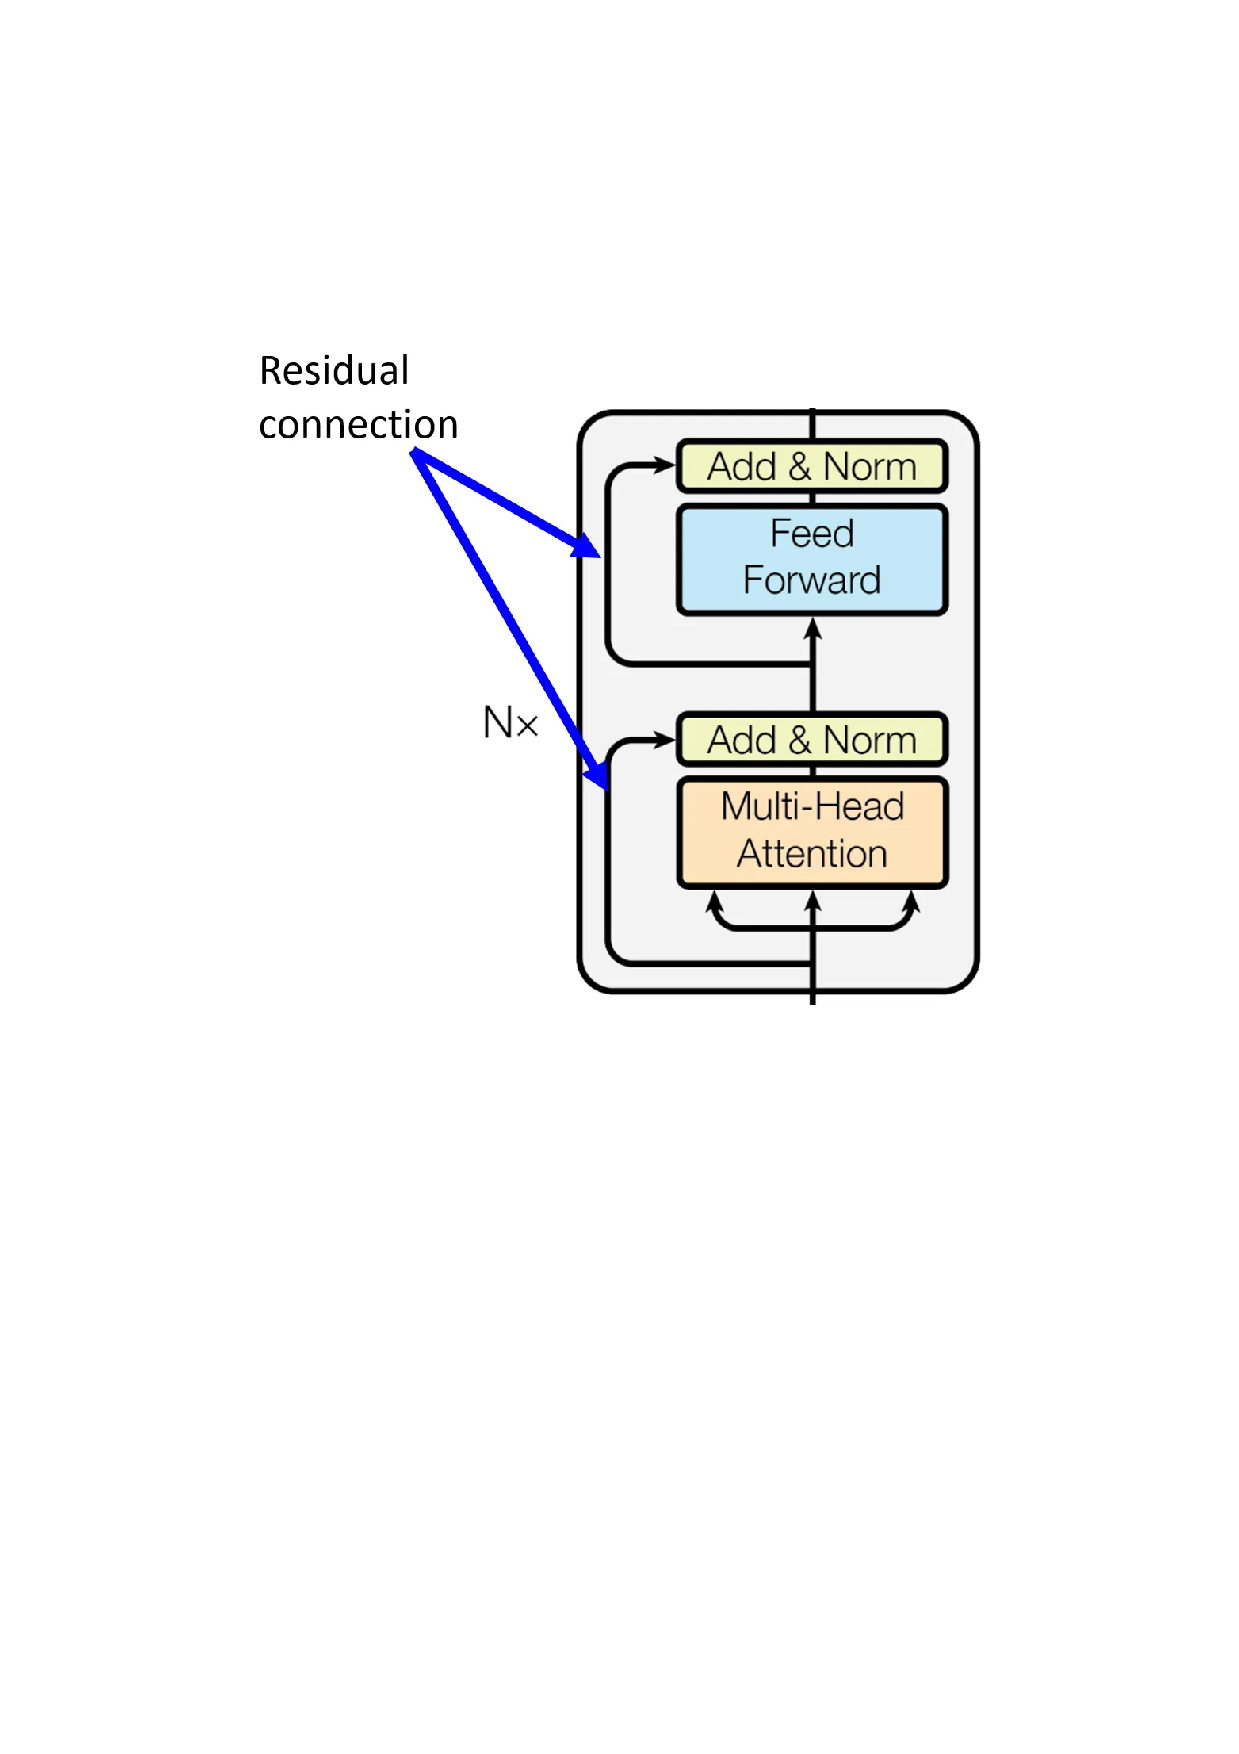
\includegraphics[width=0.8\textwidth, height=0.4\textheight]{figure/residual_connection}
                \caption{残差连接（Add）}
            \end{figure}
        \end{column}
         \begin{column}{0.7\textwidth}
         \begin{enumerate}
             \item 每个子层外均添加“残差连接”，缓解深层网络训练困难并保留原输入信息；
             \item 对于序列中任意位置的输入向量 $\symbf{x} \in \mathbb{R}^{d}$，子层的输出应满足 $\operatorname{sublayer}(\symbf{x}) \in \mathbb{R}^{d}$，以确保残差连接 $\symbf{x} + \operatorname{sublayer}(\symbf{x})$ 依然属于 $\mathbb{R}^{d}$；
             \item 梯度视角：$\frac{\partial}{\partial \symbf{x}}\left(\symbf{x}+\operatorname{sublayer}(\symbf{x})\right)=\symbf{I}+\frac{\partial \operatorname{sublayer}(\symbf{x})}{\partial \symbf{x}}$，恒等项使梯度可经捷径无衰减地直达浅层.这与 LSTM 细胞状态的加性更新（$\partial\symbf{C}_t/\partial\symbf{C}_{t-1}=\operatorname{diag}(\symbf{f}_t)$）、本实验 CNN 的残差块一脉相承——\textbf{用加性捷径对抗梯度消失}是贯穿三种架构的共同设计.
         \end{enumerate}
         \end{column}
         \end{columns}
    \item 层归一化（Layer Normalization）：原始 Transformer 采用 Add \& Norm（Post-LN），即残差相加后在特征维度上归一化；现代实现也常采用 Pre-LN 变体（先归一化再进子层，残差主路径上无归一化阻隔）以改善深层训练稳定性.\textbf{本实验实现即采用 Pre-LN}，并在编码器堆叠末端补一层 LayerNorm 以归一化最终输出；
    \item 基于位置的前馈全连接网络（Position-wise Fully Connected Feed-Forward Networks）：对序列中每个位置的表示，独立、相同地应用前馈网络\footcite{soyalpImprovingTextClassification2021,vaswaniAttentionAllYou2017}：
    \begin{equation*}
        \mathrm{FFN}(\symbf{x}) = \symbf{W}_{2} \max(0, \symbf{W}_{1} \symbf{x} + \symbf{b}_{1}) + \symbf{b}_{2}
    \end{equation*}
    分工视角：注意力子层对各位置的值向量做数据相关的凸组合，负责\textbf{跨位置的信息交换}；FFN 先升维再降维（本实验 $128\to256\to128$），提供块内主要的\textbf{非线性变换}能力——逐位置独立计算、跨位置共享参数.
\end{itemize}
\end{frame}
\section{各模型在文本分类中的应用}
\subsection{文本分类任务的通用流程}
\begin{frame}\frametitle{文本分类任务的通用流程}
\footnotesize
在使用神经网络进行文本分类任务时，通常遵循以下流程\footcite{raoActionablePoliticalText2016,wangLSTMApproachShort2018}：
\begin{enumerate}
    \item \textbf{文本预处理}：对原始文本进行规范化处理，通常包括分词、大小写归一化、截断或填充等；去除停用词、词干提取等操作应视任务而定，因为情感词或功能词有时也包含分类信息.本实验在过滤停用词时豁免否定词以保留情感信号；后文 SST-5 实验将进一步表明，程度副词（very/too 等）的过滤对细粒度情感分类有害——预处理选择与任务粒度存在交互；
    \item \textbf{词嵌入层}：
    \begin{itemize}
        \item 将离散的词汇编码为连续的低维向量，以保留词语的语义和上下文信息；
        \item 可采用预训练模型（如 \texttt{word2vec}、\texttt{GloVe}）或随机初始化后训练；
        \item 最终得到一个词向量序列（$\symbf{X}\in\mathbb{R}^{T\times d}$，$T$ 为序列长度，$d$ 为嵌入维度）.
    \end{itemize}
    \item \textbf{网络层}：输入词嵌入序列，通过 LSTM、CNN 或 Transformer 等模型提取语义特征；
    \begin{itemize}
        \item 可选结构包括单向LSTM与双向LSTM（即BiLSTM，可同时整合前向与后向语境）、CNN、Transformer 等；
        \item 采用LSTM时，常用的特征提取策略包括：
        \begin{itemize}
            \item \emph{最终隐藏状态}：取最后一个时间步的隐藏向量 $\symbf{h}_{T}$（本实验的 BiLSTM 即拼接前向与后向的最终隐藏状态）；
            \item \emph{时间步池化}：对所有时间步的隐藏状态进行最大池化或平均池化；
            \item \emph{注意力机制\footcite{baiTextClassificationBased2018}}：根据注意力权重对各时间步输出进行加权汇聚，从而聚焦于更关键的信息片段.
        \end{itemize}
    \end{itemize}
    \item \textbf{全连接与输出层}：将聚合得到的定长特征向量输入至全连接层得到 logits；训练时交叉熵可直接使用 logits，推理时再通过 Softmax 得到类别概率分布.
\end{enumerate}
\end{frame}
\subsection{CNN在文本分类中的应用}
\begin{frame}\frametitle{CNN在文本分类中的应用}
    \begin{figure}[H]
        \centering
         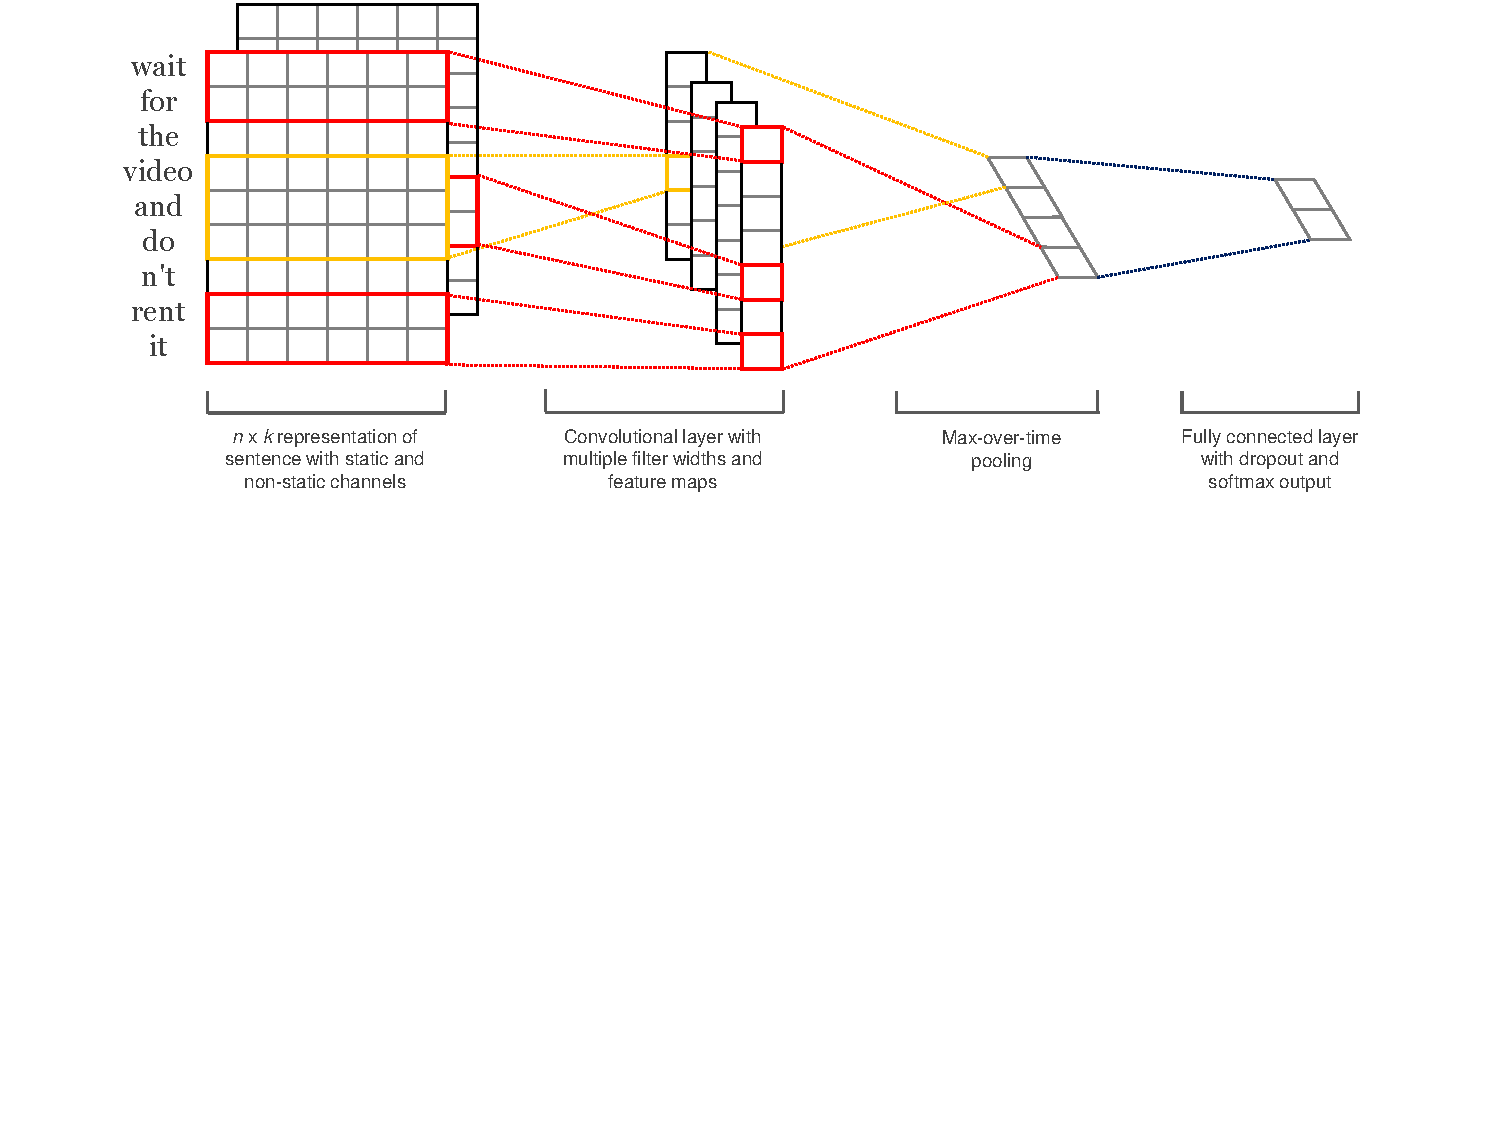
\includegraphics[width=\textwidth, height =0.35\textheight]{figure/cnn_for_text_classification}
        \caption{CNN 用于文本分类的典型结构}
    \end{figure}
    \begin{enumerate}
        \fontsize{8pt}{10pt}\selectfont
        \item \textbf{输入层}：
        设$\symbf{x}_{i} \in \mathbb{R}^k$为句中第$i$个词的$k$维词向量（word embedding），则长度为$n$的句子表示为一个矩阵：
        $\symbf{x}_{1:n} = \symbf{x}_1 \oplus \symbf{x}_2 \oplus \cdots \oplus \symbf{x}_n \in \mathbb{R}^{n \times k}$，其中 $\oplus$ 表示按行拼接.
        若实际长度不足$n$，则使用零向量填充；若超过$n$，则需截断或分段处理；
        \item \textbf{1D卷积层}：
        设二维卷积核为 $\symbf{w} \in \mathbb{R}^{h \times k}$.
        其仅在输入句子的“时间步”维度上滑动（故被称为1D卷积），每次作用于连续的 $h$ 个词向量（滑动窗口为$h$）：
        $c_{i} = f\left(\symbf{w} \cdot \symbf{x}_{i:i+h-1} + b\right)$，其中$\cdot$表示两矩阵对应元素乘积之和（Frobenius 内积），$f$为非线性激活函数（如 ReLU 或 tanh）.
        得到对应的特征图：$\symbf{c} = [c_1, c_2, \cdots, c_{n-h+1}]$；
        \item \textbf{1D池化层}：
        对每个特征图执行“时间最大池化”（max-over-time pooling）：$\hat{c} = \max_{1\le i\le n-h+1} c_i$，拼接可得固定长度的特征向量；
    \item \textbf{全连接层和输出层}：
        将所有池化后的特征拼接成一个向量输入到全连接层，使用Dropout正则化以防止过拟合.最终得到分类 logits，推理时通过Softmax输出各类别的预测概率.
    \end{enumerate}
\textbf{注意：}
\begin{enumerate}
    \item 可采用双通道词向量输入（\texttt{预训练词向量：word2vec}）
    \begin{itemize}
        \item static通道：采用预训练词向量作为输入，并在训练过程中保持不变；
        \item non-static通道：初始化时仍使用预训练词向量，但允许在训练过程中对其进行微调（fine-tuning）.
        \item 对于未在预训练词向量中的单词，则使用随机初始化.
    \end{itemize}
    \item 多个不同大小的卷积核可以提取不同 $n$-gram（由连续 $n$ 个词或字符组成的子序列）级别的特征.\footcite{kimConvolutionalNeuralNetworks2014}
    \item 本实验的 CNN 在 Kim 结构基础上做了两处改动：以\textbf{残差块}替代单层卷积以利于更深的特征组合（因输入 300 通道与输出 100 通道不匹配，捷径分支采用 $1\times1$ 卷积投影而非恒等映射），并在池化拼接后加入\textbf{批归一化}；词向量采用单通道 non-static GloVe（训练中允许微调）.
\end{enumerate}
\end{frame}
\subsection{BLSTM-2DCNN简介}
\begin{frame}\frametitle{BLSTM-2DCNN简介\footcite{zhouTextClassificationImproved2016}}
\fontsize{9pt}{10pt}\selectfont
\begin{columns}
    \column{ 0.6\textwidth}
    \begin{figure}[H]
        \centering
        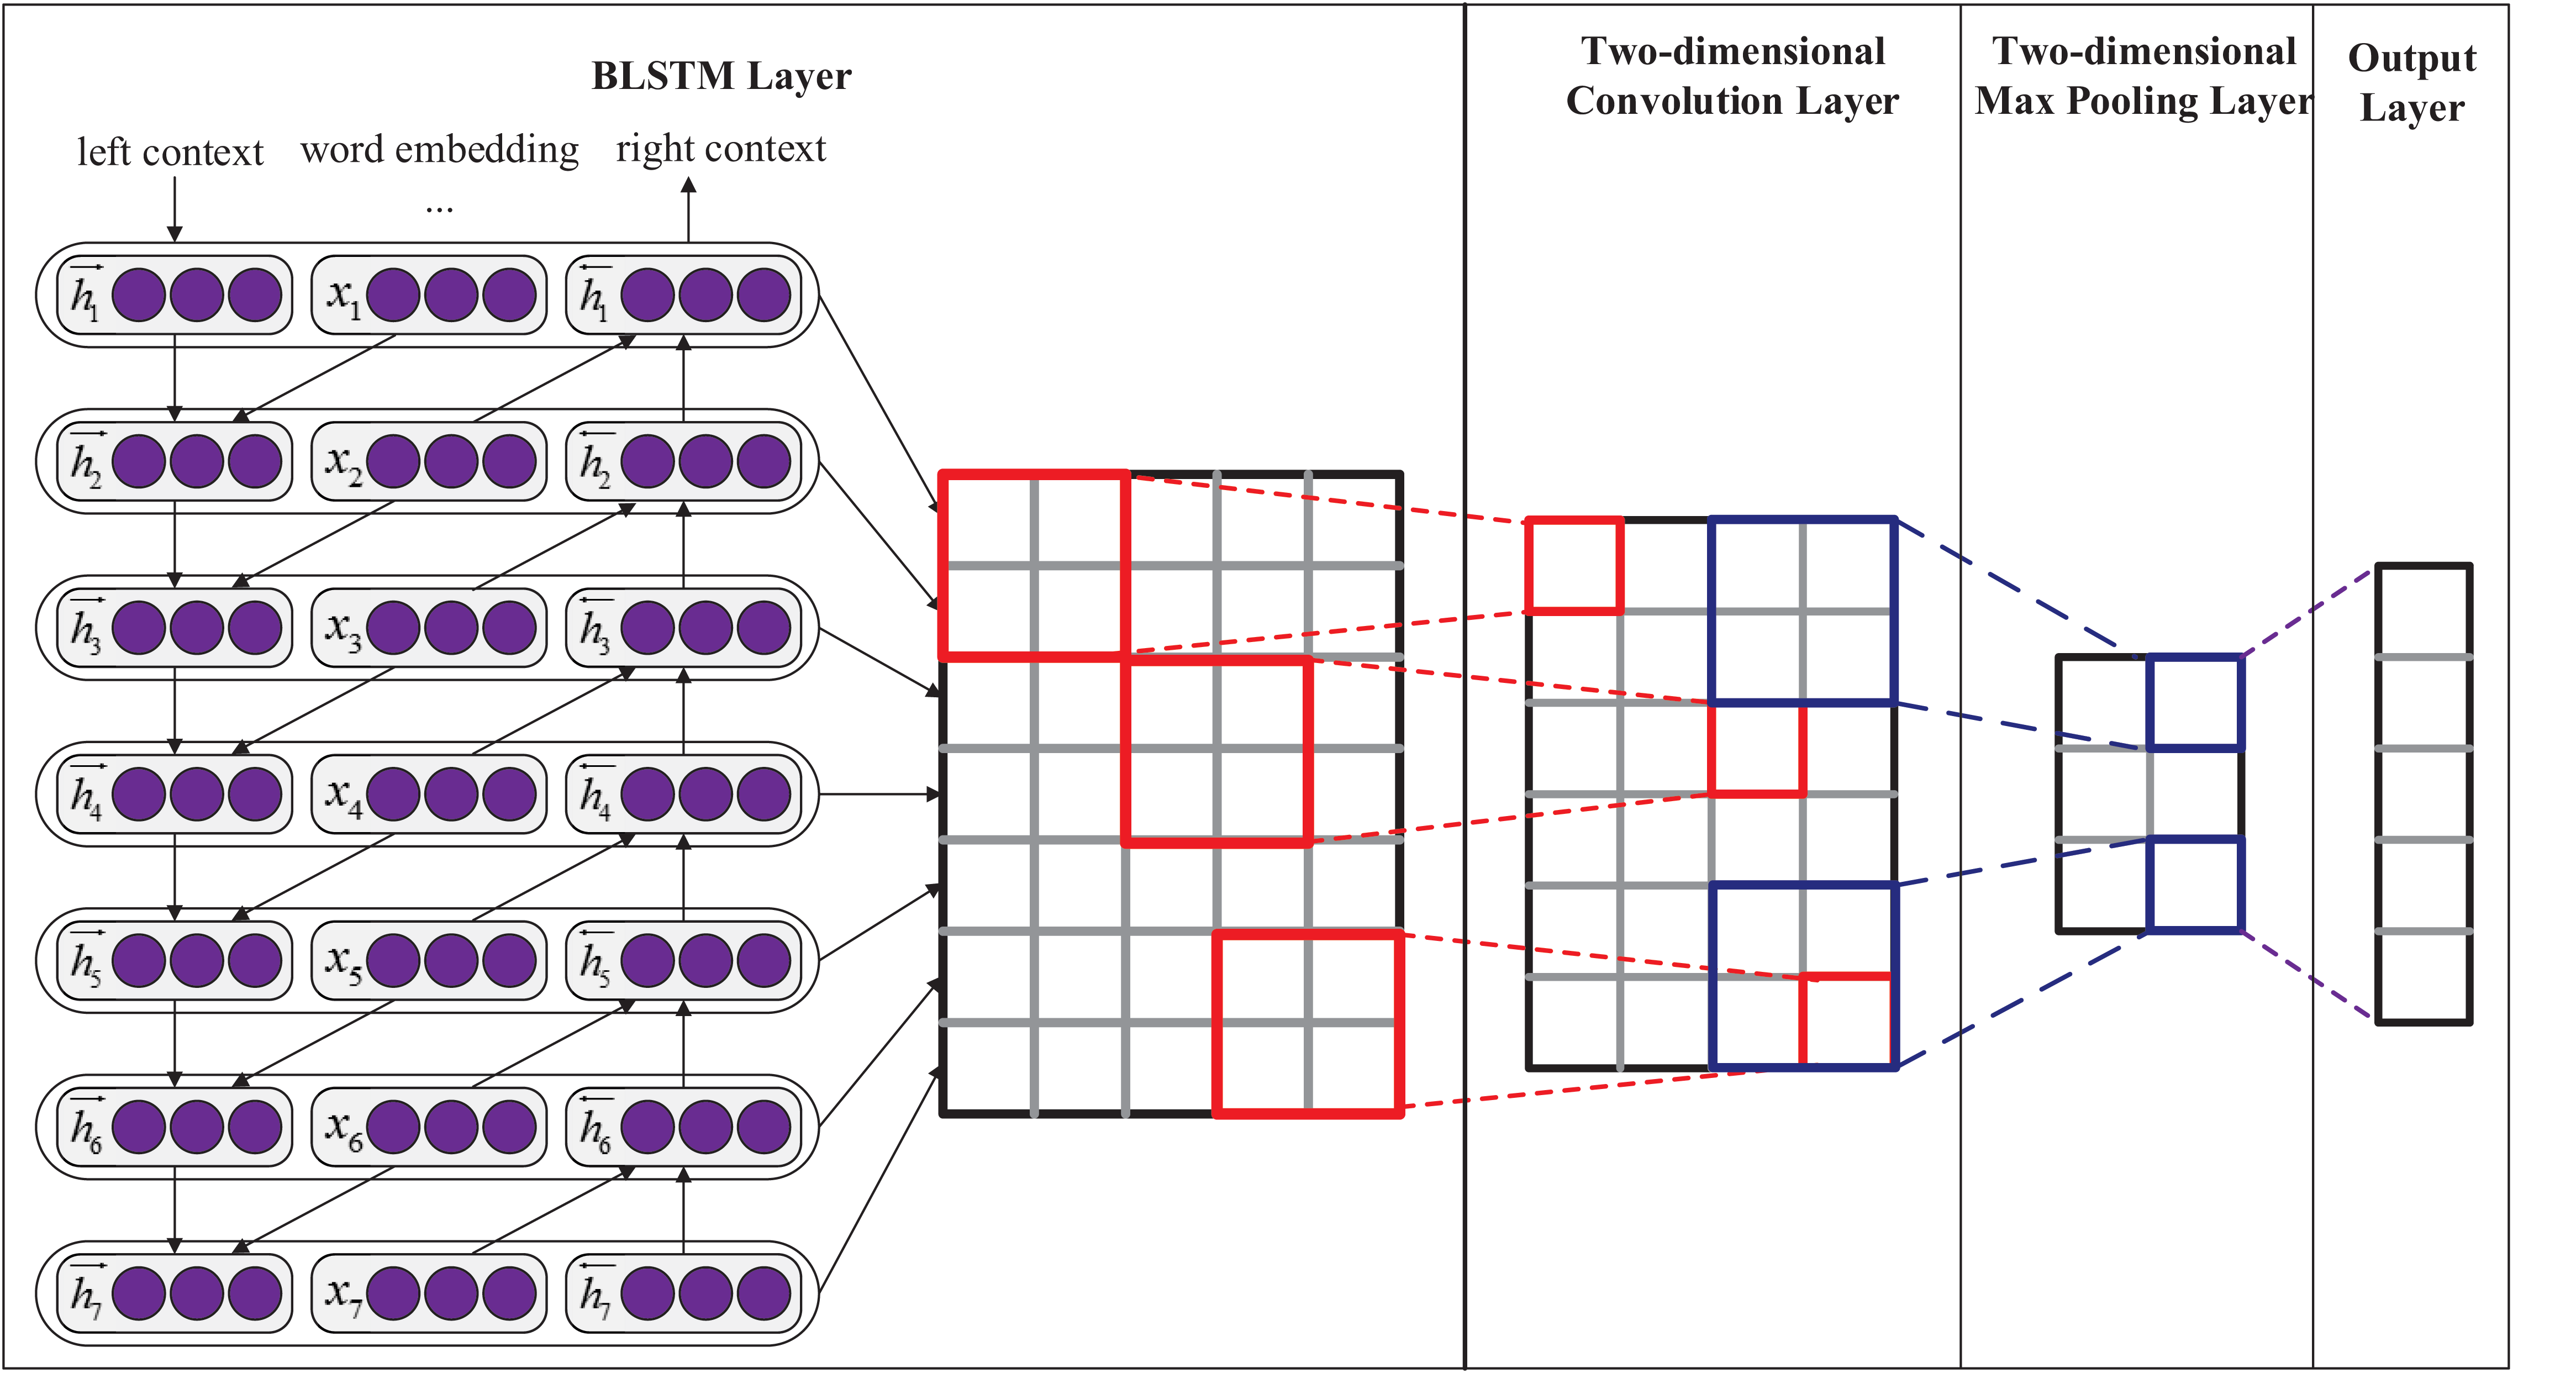
\includegraphics[width=\textwidth, height=0.30\textheight]{figure/coling2}
        \caption{BLSTM-2DCNN 模型结构}
    \end{figure}
    \begin{enumerate}
    \setcounter{enumi}{2}
        \item 2D Pooling（确保获得定长向量，并捕获“时间步”维度和特征向量维度的特征）：
        \begin{align*}
            \symbf{p}_{i,j} &= \operatorname{down}(\symbf{O}_{i:i+p_{1}-1,\,j:j+p_{2}-1})
        \end{align*}
        \item 输出层：
        \begin{align*}
            \hat{p}\left(y\mid s\right) &= \mathrm{softmax}\left(\symbf{W}^{(s)}\symbf{h}^{*}+\symbf{b}^{(s)}\right)\\
            \hat{y} &= \operatorname*{arg\,max}_{y}\, \hat{p}\left(y\mid s\right)
        \end{align*}
    \end{enumerate}
    \column{0.4\textwidth}
    \begin{enumerate}
        \item BiLSTM（捕获双向的长距离依赖，将文本转换为向量）：
\begin{align*}
\begin{bmatrix}
    \symbf{i}_{t} \\
    \symbf{f}_{t} \\
    \symbf{o}_{t} \\
    \hat{\symbf{c}}_{t}
\end{bmatrix}
    &=
\begin{bmatrix}
    \sigma \\
    \sigma \\
    \sigma \\
    \tanh
\end{bmatrix}
    \symbf{W}
    \left[\symbf{h}_{t-1}, \symbf{x}_{t}\right]\\
    \symbf{c}_{t} &= \symbf{f}_{t} \odot \symbf{c}_{t-1} + \symbf{i}_{t} \odot \hat{\symbf{c}}_{t}\\
    \symbf{h}_{t} &= \symbf{o}_{t} \odot \tanh(\symbf{c}_{t})\\
    \symbf{h}_{i} &= \left[\overrightarrow{\symbf{h}_{i}}\oplus\overleftarrow{\symbf{h}_{i}}\right]
\end{align*}
        \item  2D CNN（将双向表征融合为新的表达形式）：
        \begin{align*}
            o_{i,j} &= f\left(\symbf{m}*\symbf{H}_{i:i+k-1,j:j+d-1}+b\right)\\
            O &= \left[ o_{1,1}, \cdots, o_{l-k+1,h-d+1}\right]
        \end{align*}
    \end{enumerate}
    \end{columns}
\end{frame}
\subsection{Transformer在文本分类中的应用}
\begin{frame}\frametitle{Transformer在文本分类中的应用}
\fontsize{8pt}{10pt}\selectfont
文本分类通常仅使用编码器而非完整的编码器-解码器结构.基本流程为：
\begin{enumerate}
    \item \textbf{嵌入与位置编码}：词向量（GloVe-300d）按 $\sqrt{d_{\mathrm{model}}}$ 缩放并线性投影至 $d_{\mathrm{model}}$ 维，再叠加位置编码 $\symbf{P}$：
    \[
        \symbf{E}=\mathrm{Proj}\!\big(\sqrt{d_{\mathrm{model}}}\,\mathrm{Embedding}(\symbf{x})\big)+\symbf{P}\in\mathbb{R}^{T\times d_{\mathrm{model}}}
    \]
    \item \textbf{编码器堆叠}：利用多头自注意力和前馈网络得到上下文表示：
    \[
        \symbf{H}=\mathrm{Encoder}(\symbf{E}, \mathrm{padding\ mask})\in\mathbb{R}^{T\times d_{\mathrm{model}}}
    \]
    其中 $T$ 为序列长度，$\symbf{P}\in\mathbb{R}^{T\times d_{\mathrm{model}}}$ 为位置编码矩阵；padding mask 用于避免模型关注填充位置，分类任务一般不需要解码器中的因果 mask.
    \item \textbf{序列汇聚}：将变长序列表示转为定长向量，可使用 \texttt{[CLS]} 向量、平均池化或最大池化：
    \[
        \symbf{z}=\symbf{h}_{\mathrm{[CLS]}}\quad \text{或}\quad
        \symbf{z}=\frac{1}{|\mathcal{T}|}\sum_{t\in\mathcal{T}}\symbf{h}_t
    \]
    其中 $\mathcal{T}$ 表示非填充位置集合.本实验采用上式右侧的\textbf{掩蔽平均池化}：仅对真实词位置取平均.若不加掩蔽地对全部 $T$ 个位置平均，填充位会稀释有效信号（短文本中填充占比可达 80\% 以上），显著损害性能.
    \item \textbf{分类头}：标准做法为单层线性 $\symbf{s}=\symbf{W}_{\mathrm{cls}}\symbf{z}+\symbf{b}_{\mathrm{cls}}$；\textbf{本实验}采用三层 MLP（$d_{\mathrm{model}}\!\to\!d_{\mathrm{ff}}\!\to\!d_{\mathrm{ff}}/2\!\to\!C$，即 $128\!\to\!256\!\to\!128\!\to\!C$，每层后接 LayerNorm、ReLU 与 Dropout）：
    \[
        \hat{\symbf{y}}=\mathrm{softmax}\!\big(\mathrm{MLP}(\symbf{z})\big)
    \]
\end{enumerate}
\end{frame}
\section{模型训练}
\subsection{数据集}
\begin{frame}
\frametitle{数据集简介：IMDB、AG News、BBC News、SST-5}
\begin{table}[H]
    \centering
    \scriptsize
    \begin{tabular}{lccccc}
        \toprule
        数据集 & 任务 & 类别 & 训练/验证/测试 & 截断长度 & 特点 \\
        \midrule
        IMDB（\href{https://huggingface.co/datasets/stanfordnlp/imdb}{LINK}） & 情感二分类 & 2 & 22{,}500/2{,}500/25{,}000 & 400 & 长评论 \\
        AG News（\href{https://huggingface.co/datasets/fancyzhx/ag_news}{LINK}） & 主题分类 & 4 & 108{,}000/12{,}000/7{,}600 & 64 & 短新闻、大规模 \\
        BBC News（\href{https://huggingface.co/datasets/SetFit/bbc-news}{LINK}） & 主题分类 & 5 & 980/245/1{,}000 & 512 & 长文档、小样本 \\
        SST-5（\href{https://huggingface.co/datasets/SetFit/sst5}{LINK}） & 细粒度情感 & 5 & 7{,}689/855/2{,}210 & 64 & 句子级、高难度 \\
        \bottomrule
    \end{tabular}
\end{table}
\begin{itemize}
    \fontsize{9pt}{11pt}\selectfont
    \item 四个数据集在\textbf{数据规模}（980 -- 10.8万）、\textbf{文本长度}（句子级 -- 长文档）、\textbf{任务难度}（二分类 -- 五级细粒度情感）三个维度上互补，便于归因架构差异；
    \item 全部经 Hugging Face Hub 自动下载；训练集按 9:1 分层抽样切分验证集（BBC 因样本极少按 8:2）；
    \item 验证集驱动早停、学习率调度与最佳模型选择，\textbf{测试集仅在训练结束后评估一次}；词表仅由训练子集构建，避免信息泄漏；
    \item 预处理：小写化、去除 HTML/URL/非字母字符、词级切分、过滤停用词（否定词如 not/no/don 豁免，保留情感信号）与单字符词；词向量采用 GloVe-6B-300d，未命中词随机初始化.
\end{itemize}
\end{frame}
\subsection{损失函数与优化策略}
\begin{frame}\frametitle{损失函数：多分类交叉熵 \quad 优化策略：AdamW算法}
{\fontsize{9pt}{11pt}\selectfont 多分类交叉熵损失（$N$ 为样本数，$C$ 为类别数；$\symbf{s}_i$ 为第 $i$ 个样本的 logits，$\hat{y}_{i,c}=\mathrm{softmax}(\symbf{s}_i)_c$ 为预测概率，$y_{i,c}\in\{0,1\}$ 为 one-hot 标签分量）：}
\begin{align*}
L(\symbf{y}, \hat{\symbf{y}}) = - \frac{1}{N} \sum_{i=1}^{N} \sum_{c=1}^{C} y_{i,c} \log \hat{y}_{i,c}
\end{align*}
{\fontsize{9pt}{11pt}\selectfont AdamW 在 Adam 的自适应学习率基础上将权重衰减与梯度更新解耦（$\symbf{g}_t$ 为小批量梯度，$\beta_1,\beta_2\in[0,1)$ 为衰减系数，$\epsilon>0$ 为数值稳定项；平方、开方、除法均为逐元素运算）：}
\begin{align*}
\symbf{m}_t &= \beta_1\symbf{m}_{t-1}+(1-\beta_1)\symbf{g}_t,\quad
\symbf{v}_t = \beta_2\symbf{v}_{t-1}+(1-\beta_2)\,\symbf{g}_t\odot\symbf{g}_t\\
\hat{\symbf{m}}_t &= \frac{\symbf{m}_t}{1-\beta_1^t},\quad
\hat{\symbf{v}}_t = \frac{\symbf{v}_t}{1-\beta_2^t},\quad
\symbf{\theta}_{t+1}=\symbf{\theta}_t-\eta\left(\frac{\hat{\symbf{m}}_t}{\sqrt{\hat{\symbf{v}}_t}+\epsilon}+\lambda\symbf{\theta}_t\right)
\end{align*}
{\fontsize{9pt}{11pt}\selectfont 为何解耦：若把衰减写成 L2 正则并入梯度（Adam+L2），$\lambda\symbf{\theta}$ 会进入 $\symbf{m}_t,\symbf{v}_t$ 并被自适应分母 $\sqrt{\hat{\symbf{v}}_t}$ 缩放——历史梯度越大的参数受到的正则反而越弱；AdamW 将衰减项移出自适应机制（上式末项），使所有参数受到一致的乘性收缩，正则强度不随梯度尺度漂移.}
\newpage
\textbf{统一训练协议}（三模型完全一致，保证比较公平）：
\begin{itemize}
    \fontsize{9pt}{11pt}\selectfont
    \item AdamW（$\eta=10^{-3}$，权重衰减 $\lambda=0.01$）+ 梯度裁剪（max-norm 1.0，防止 LSTM 梯度爆炸）；
    \item ReduceLROnPlateau 调度（验证损失 2 轮无改善则学习率减半）；
    \item 早停：验证损失连续 5 轮改善不足 $10^{-3}$ 即停止（上限 50 轮），按最优验证损失回溯模型权重.
\end{itemize}
\end{frame}
\section{性能比较}
\subsection{IMDB情感分类}
\begin{frame}\frametitle{IMDB情感分类任务中三种模型的性能比较}
\begin{table}[H]
    \centering
    \fontsize{6pt}{7pt}\selectfont
    \resizebox{\textwidth}{!}{
    \begin{tabular}{lccc}
        \toprule
        \multicolumn{4}{c}{\textbf{IMDB 数据集：统一训练协议下的性能对比（RTX 5090 $\times$1）}} \\
        \midrule
        \textbf{统一超参数} & \multicolumn{3}{l}{
            \begin{tabular}[c]{@{}l@{}}
                Batch Size: 512, \quad AdamW ($\eta=10^{-3}$, $\lambda=0.01$), \quad Max Epochs: 50 + Early Stopping, \\
                Grad Clip: 1.0, \quad GloVe-300d, \quad Max Length: 400, \quad Random Seed: 42.
            \end{tabular}
        } \\
        \midrule
        \textbf{指标} & BiLSTM & \textbf{\textcolor{blue}{CNN}} & Transformer \\
        \midrule
        Test Accuracy & 87.3\% & \textcolor{blue}{88.5\%} & 88.1\% \\
        Test F1-Score & 87.3\% & \textcolor{blue}{88.4\%} & 88.1\% \\
        Test Loss & 0.3536 & 0.2917 & \textcolor{blue}{0.2865} \\
        Val Accuracy & 90.1\% & 89.4\% & 88.3\% \\
        Hidden Dim & 128 & -- & -- \\
        Layers & 2 & -- & 2 \\
        Dropout & 0.5 & 0.5 & 0.1 \\
        Filters / Kernels & -- & 100 / [2,3,4] & -- \\
        Model Dim / Heads / FFN & -- & -- & 128 / 4 / 256 \\
        Samples/s (Inference) & 34{,}221 & \textcolor{blue}{51{,}636} & 27{,}633 \\
        \bottomrule
    \end{tabular}
    }
    \label{tab:cmp-imdb}
\end{table}
\newpage
\begin{columns}
\begin{column}{0.7\textwidth}
    \centering
    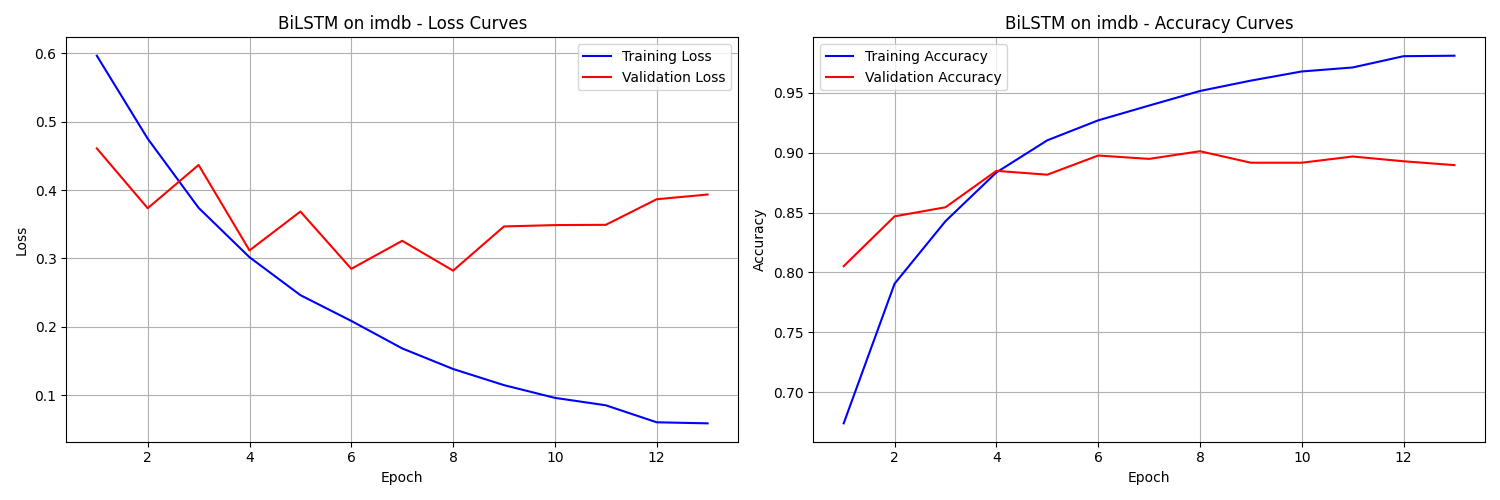
\includegraphics[width=0.9\textwidth, height=0.26\textheight]{figure/plots/BiLSTM_imdb_training_curves}
    \vspace{-2pt}
    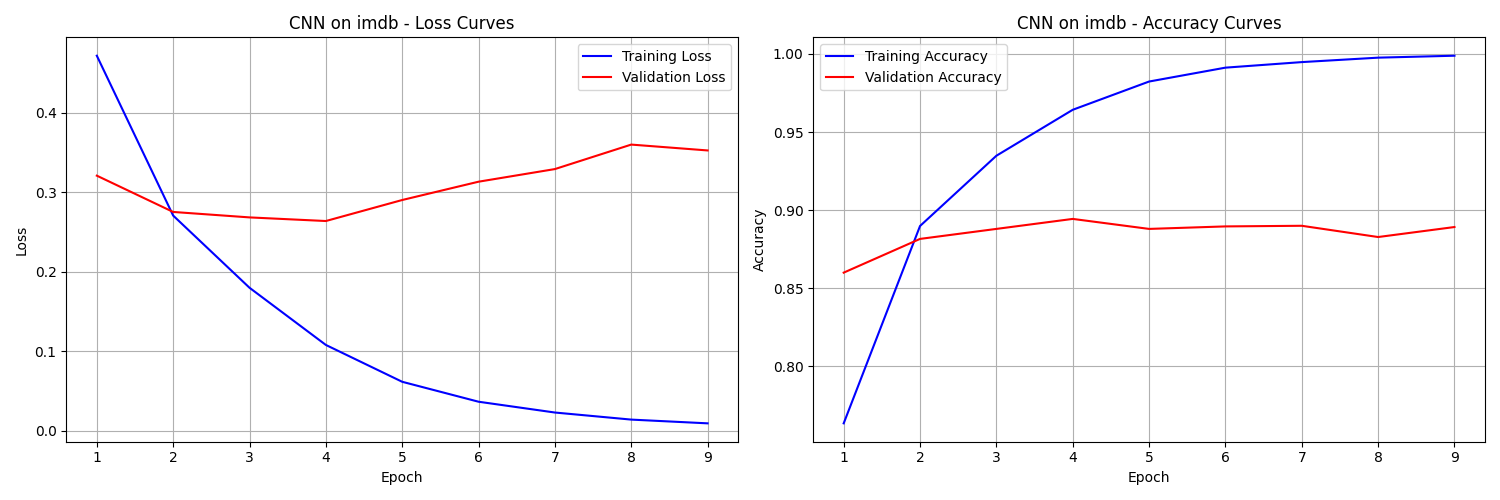
\includegraphics[width=0.9\textwidth, height=0.26\textheight]{figure/plots/CNN_imdb_training_curves}
    \vspace{-2pt}
    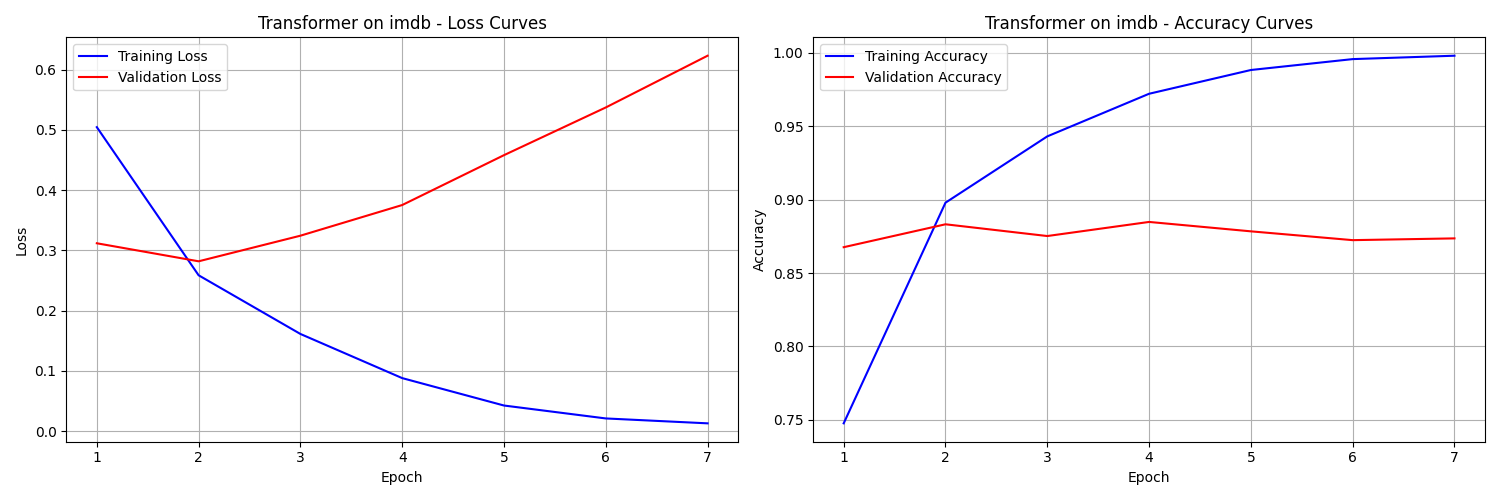
\includegraphics[width=0.9\textwidth, height=0.26\textheight]{figure/plots/Transformer_imdb_training_curves}
    \captionof{figure}{三种模型在 IMDB 上的训练与验证曲线（自上而下：BiLSTM、CNN、Transformer）}
\end{column}
\begin{column}{0.3\textwidth}
\begin{table}[H]
    \centering
    \scriptsize
    \begin{tabular}{lc}
        \toprule
        \multicolumn{2}{c}{\textbf{数据划分}} \\
        \midrule
        训练集 & 22{,}500 \\
        验证集 & 2{,}500 \\
        测试集 & 25{,}000 \\
        \bottomrule
    \end{tabular}
\end{table}
\begin{enumerate}
    \fontsize{7pt}{9pt}\selectfont
    \setlength{\itemsep}{2pt}
    \item CNN（88.5\%）与 Transformer（88.1\%）领先 BiLSTM（87.3\%）：影评情感判别强依赖局部 n-gram 线索（如 ``not good''），契合卷积的归纳偏置；
    \item 停用词过滤使截断窗口内的有效上下文接近翻倍，Transformer 从更完整的全局语义中获益，与 CNN 差距缩小至 0.4 个百分点；
    \item 三模型早停分别在第 13、9、7 轮触发，训练--验证--测试三级指标梯度合理，过拟合受控.
\end{enumerate}
\end{column}
    \end{columns}
\end{frame}

\subsection{AG News新闻分类}
\begin{frame}\frametitle{AG News新闻分类任务中三种模型的性能比较}
\begin{table}[H]
    \centering
    \fontsize{6pt}{7pt}\selectfont
    \resizebox{\textwidth}{!}{
    \begin{tabular}{lccc}
        \toprule
        \multicolumn{4}{c}{\textbf{AG News 数据集：统一训练协议下的性能对比（RTX 5090 $\times$1）}} \\
        \midrule
        \textbf{统一超参数} & \multicolumn{3}{l}{
            \begin{tabular}[c]{@{}l@{}}
                Batch Size: 512, \quad AdamW ($\eta=10^{-3}$, $\lambda=0.01$), \quad Max Epochs: 50 + Early Stopping, \\
                Grad Clip: 1.0, \quad GloVe-300d, \quad Max Length: 64, \quad Random Seed: 42.
            \end{tabular}
        } \\
        \midrule
        \textbf{指标} & BiLSTM & CNN & Transformer \\
        \midrule
        Test Accuracy & 92.3\% & 92.2\% & 92.1\% \\
        Test F1-Score & 92.3\% & 92.1\% & 92.1\% \\
        Test Loss & \textcolor{blue}{0.2259} & 0.2380 & 0.2365 \\
        Val Accuracy & 93.0\% & 92.8\% & 92.5\% \\
        Hidden Dim & 128 & -- & -- \\
        Layers & 2 & -- & 2 \\
        Dropout & 0.5 & 0.5 & 0.1 \\
        Filters / Kernels & -- & 100 / [2,3,4] & -- \\
        Model Dim / Heads / FFN & -- & -- & 128 / 4 / 256 \\
        Samples/s (Inference) & 171{,}914 & \textcolor{blue}{342{,}039} & 300{,}090 \\
        \bottomrule
    \end{tabular}
    }
    \label{tab:cmp-agnews}
\end{table}
\newpage
\begin{columns}
\begin{column}{0.7\textwidth}
    \centering
    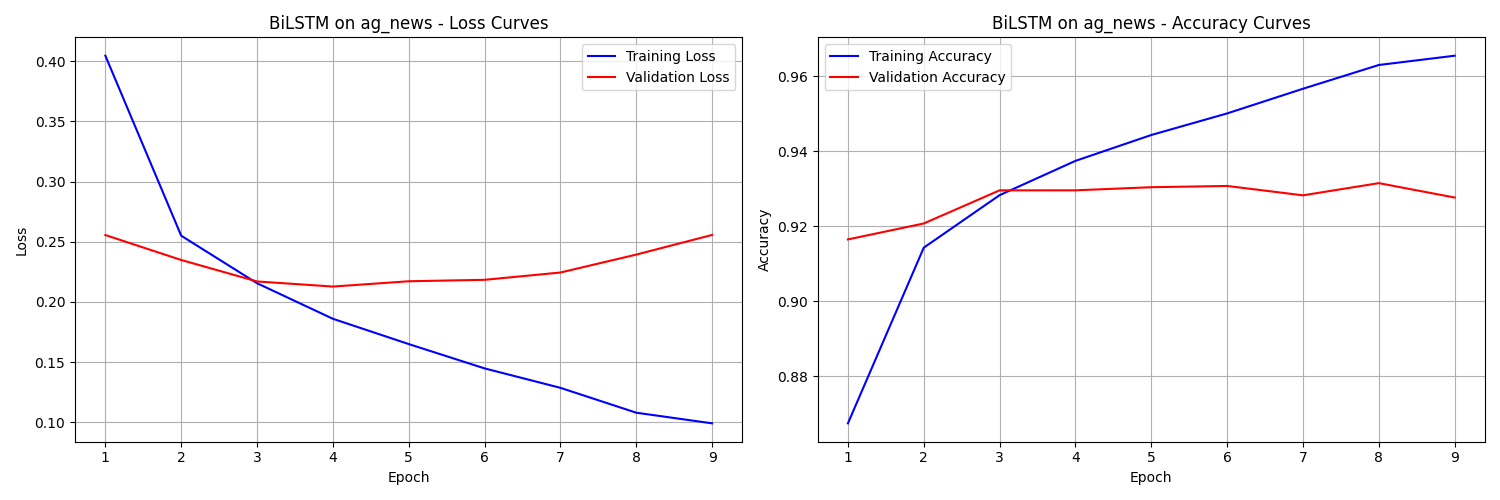
\includegraphics[width=0.9\textwidth, height=0.26\textheight]{figure/plots/BiLSTM_ag_news_training_curves}
    \vspace{-2pt}
    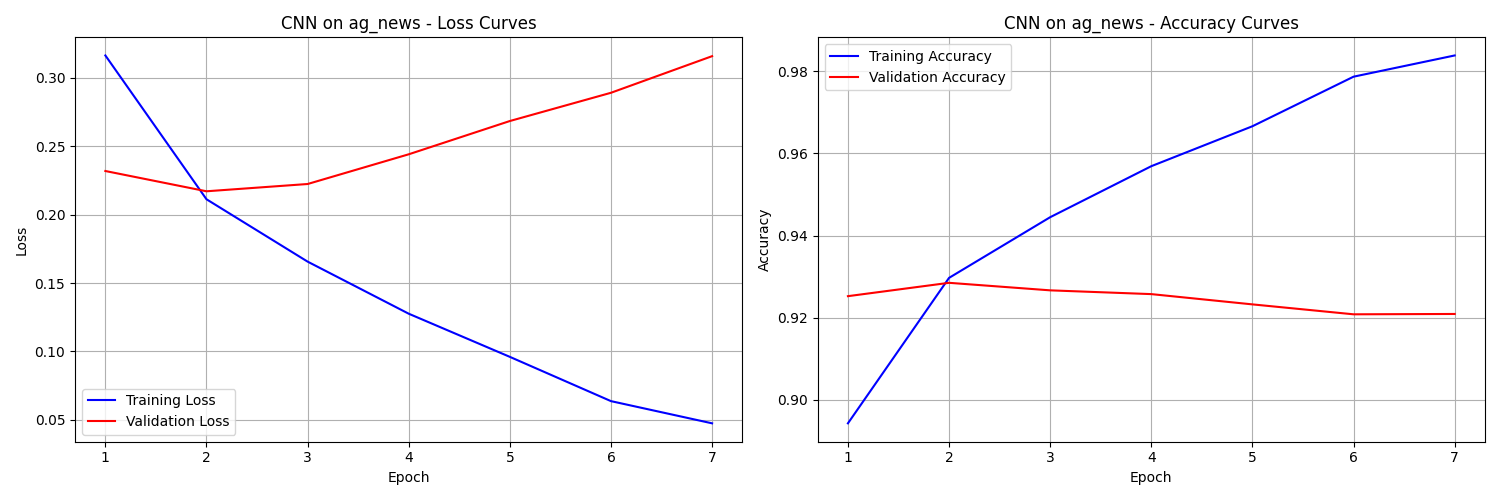
\includegraphics[width=0.9\textwidth, height=0.26\textheight]{figure/plots/CNN_ag_news_training_curves}
    \vspace{-2pt}
    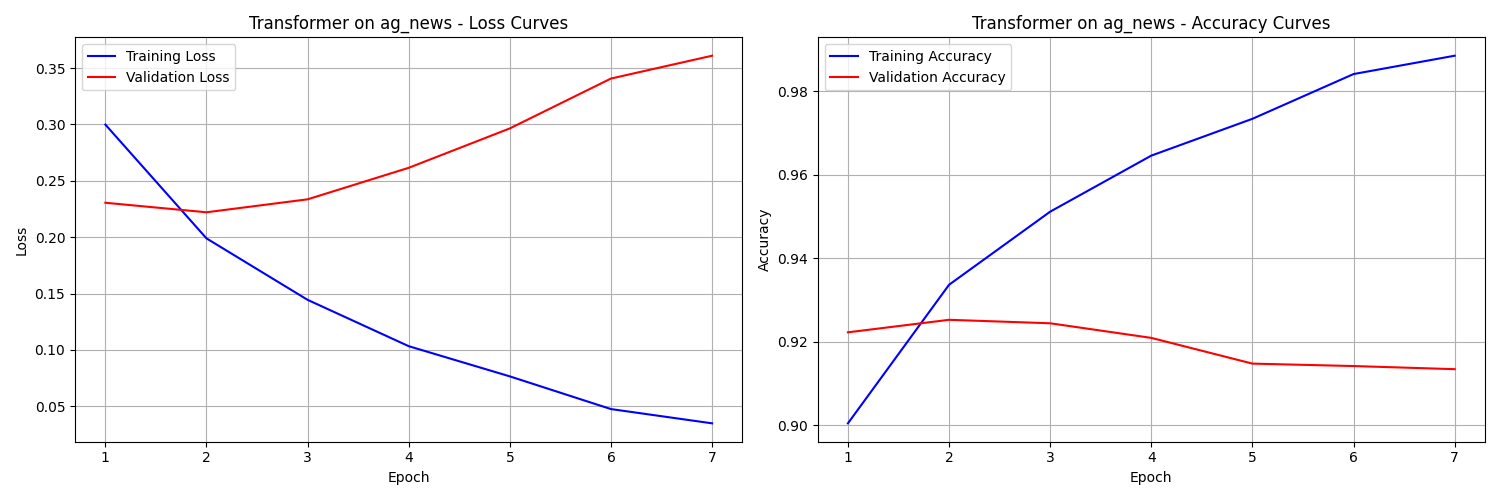
\includegraphics[width=0.9\textwidth, height=0.26\textheight]{figure/plots/Transformer_ag_news_training_curves}
    \captionof{figure}{三种模型在 AG News 上的训练与验证曲线（自上而下：BiLSTM、CNN、Transformer）}
\end{column}
\begin{column}{0.3\textwidth}
\begin{table}[H]
    \centering
    \scriptsize
    \begin{tabular}{lc}
        \toprule
        \multicolumn{2}{c}{\textbf{数据划分}} \\
        \midrule
        训练集 & 108{,}000 \\
        验证集 & 12{,}000 \\
        测试集 & 7{,}600 \\
        \bottomrule
    \end{tabular}
\end{table}
\begin{enumerate}
    \fontsize{7pt}{9pt}\selectfont
    \setlength{\itemsep}{2pt}
    \item 三模型测试准确率 92.1\%--92.3\%，差距小于测试集的统计噪声（标准误约 $\pm$0.3\%），应视为\textbf{无显著差异}；
    \item 短新闻的主题判别主要依赖关键词（体育、商业等领域词汇），任何架构均可充分捕捉——数据充足且文本短时，架构选择影响甚微；
    \item 短序列（64 词）下并行架构的推理吞吐优势显著：CNN 34.2万、Transformer 30.0万、BiLSTM 17.2万 samples/s，顺序计算成为 BiLSTM 的瓶颈.
\end{enumerate}
\end{column}
    \end{columns}
\end{frame}
\subsection{BBC News新闻分类}
\begin{frame}\frametitle{BBC News新闻分类任务中三种模型的性能比较}
\begin{table}[H]
    \centering
    \fontsize{6pt}{7pt}\selectfont
    \resizebox{\textwidth}{!}{
    \begin{tabular}{lccc}
        \toprule
        \multicolumn{4}{c}{\textbf{BBC News 数据集：统一训练协议下的性能对比（RTX 5090 $\times$1）}} \\
        \midrule
        \textbf{统一超参数} & \multicolumn{3}{l}{
            \begin{tabular}[c]{@{}l@{}}
                Batch Size: 512, \quad AdamW ($\eta=10^{-3}$, $\lambda=0.01$), \quad Max Epochs: 50 + Early Stopping, \\
                Grad Clip: 1.0, \quad GloVe-300d, \quad Max Length: 512, \quad Random Seed: 42.
            \end{tabular}
        } \\
        \midrule
        \textbf{指标} & \textbf{\textcolor{red}{BiLSTM}} & \textbf{\textcolor{blue}{CNN}} & Transformer \\
        \midrule
        Test Accuracy & \textcolor{red}{94.8\%} & \textcolor{blue}{97.3\%} & 96.3\% \\
        Test F1-Score & \textcolor{red}{94.8\%} & \textcolor{blue}{97.3\%} & 96.3\% \\
        Test Loss & 0.2037 & \textcolor{blue}{0.0845} & 0.1225 \\
        Val Accuracy & 97.6\% & 97.1\% & 98.0\% \\
        Hidden Dim & 128 & -- & -- \\
        Layers & 2 & -- & 2 \\
        Dropout & 0.5 & 0.5 & 0.1 \\
        Filters / Kernels & -- & 100 / [2,3,4] & -- \\
        Model Dim / Heads / FFN & -- & -- & 128 / 4 / 256 \\
        Samples/s (Inference) & 27{,}262 & \textcolor{blue}{40{,}910} & \textcolor{red}{19{,}726} \\
        \bottomrule
    \end{tabular}
    }
    \label{tab:cmp-bbc}
\end{table}
\newpage
\begin{columns}
\begin{column}{0.7\textwidth}
    \centering
    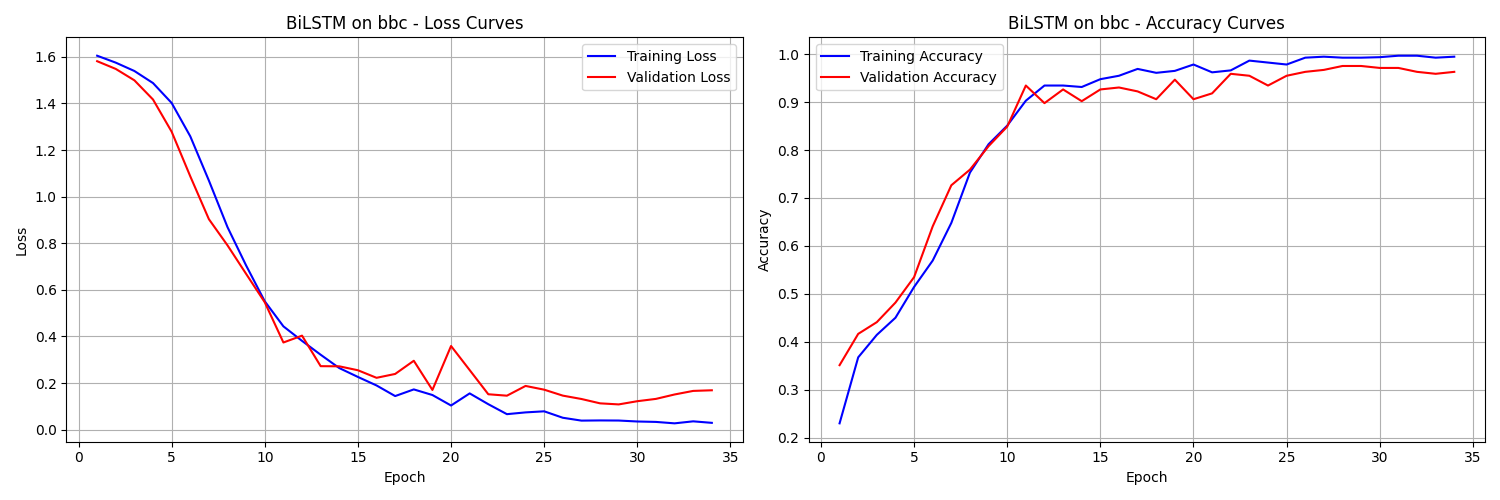
\includegraphics[width=0.9\textwidth, height=0.26\textheight]{figure/plots/BiLSTM_bbc_training_curves}
    \vspace{-2pt}
    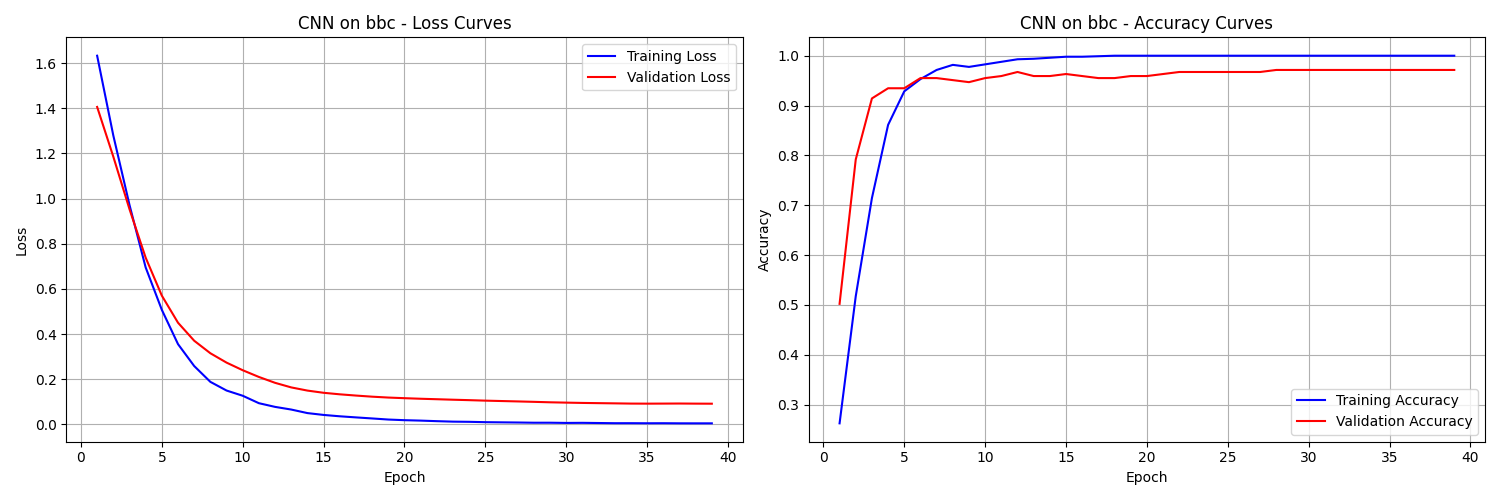
\includegraphics[width=0.9\textwidth, height=0.26\textheight]{figure/plots/CNN_bbc_training_curves}
    \vspace{-2pt}
    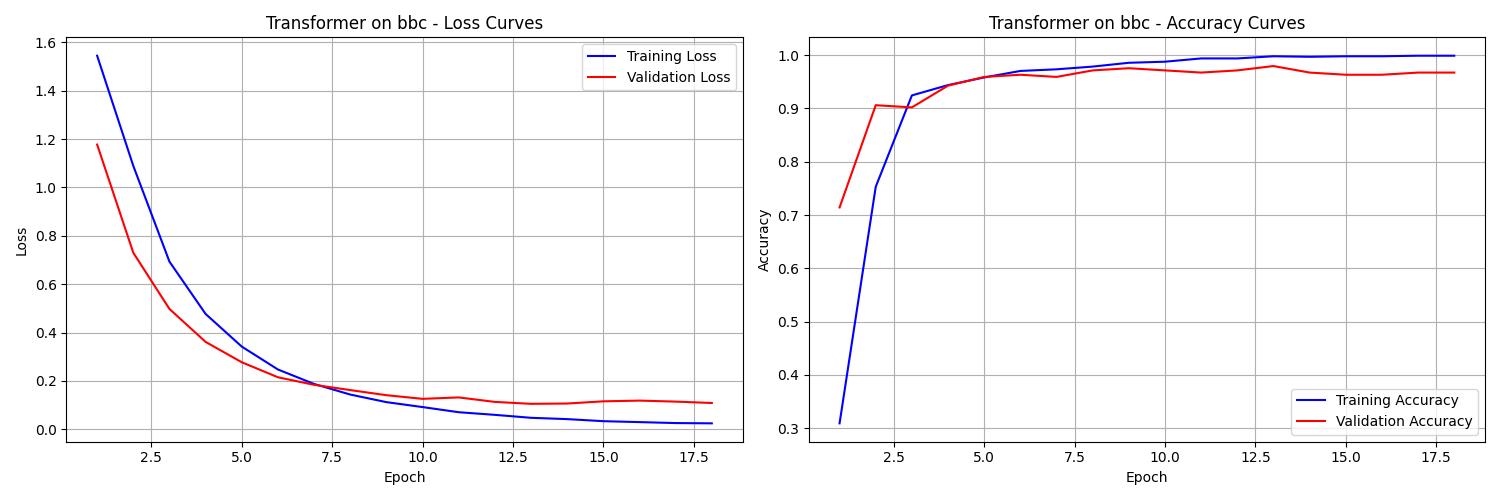
\includegraphics[width=0.9\textwidth, height=0.26\textheight]{figure/plots/Transformer_bbc_training_curves}
    \captionof{figure}{三种模型在 BBC News 上的训练与验证曲线（自上而下：BiLSTM、CNN、Transformer）}
\end{column}
\begin{column}{0.3\textwidth}
\begin{table}[H]
    \centering
    \scriptsize
    \begin{tabular}{lc}
        \toprule
        \multicolumn{2}{c}{\textbf{数据划分}} \\
        \midrule
        训练集 & 980 \\
        验证集 & 245 \\
        测试集 & 1{,}000 \\
        \bottomrule
    \end{tabular}
\end{table}
\begin{enumerate}
    \fontsize{7pt}{9pt}\selectfont
    \setlength{\itemsep}{2pt}
    \item 仅 980 条训练样本、每轮 2 个批次的极端小样本场景下，BiLSTM 过拟合最重（测试 94.8\%，落后 2.5 个百分点），体现循环结构的样本效率劣势；
    \item CNN 与 Transformer 凭借并行特征提取仍快速收敛至 96\%--97\%；
    \item 长文档（截断 512 词）下 Transformer 推理吞吐降至三者最低（约 2.0万 samples/s），自注意力 $\mathcal{O}(n^2)$ 复杂度开始显现，与后文原理分析一致；
    \item 验证集仅 245 条，曲线波动较大，结论需结合测试集（1{,}000 条）解读.
\end{enumerate}
\end{column}
    \end{columns}
\end{frame}
\subsection{SST-5细粒度情感分类}
\begin{frame}\frametitle{SST-5细粒度情感分类任务中三种模型的性能比较}
\begin{table}[H]
    \centering
    \fontsize{6pt}{7pt}\selectfont
    \resizebox{\textwidth}{!}{
    \begin{tabular}{lccc}
        \toprule
        \multicolumn{4}{c}{\textbf{SST-5 数据集：统一训练协议下的性能对比（RTX 5090 $\times$1）}} \\
        \midrule
        \textbf{统一超参数} & \multicolumn{3}{l}{
            \begin{tabular}[c]{@{}l@{}}
                Batch Size: 512, \quad AdamW ($\eta=10^{-3}$, $\lambda=0.01$), \quad Max Epochs: 50 + Early Stopping, \\
                Grad Clip: 1.0, \quad GloVe-300d, \quad Max Length: 64, \quad Random Seed: 42.
            \end{tabular}
        } \\
        \midrule
        \textbf{指标} & BiLSTM & CNN & Transformer \\
        \midrule
        Test Accuracy & 41.9\% & 42.4\% & 42.4\% \\
        Test F1-Score & 37.4\% & \textcolor{blue}{38.6\%} & 38.3\% \\
        Test Loss & 1.3208 & \textcolor{blue}{1.2998} & 1.3219 \\
        Val Accuracy & 41.6\% & 41.4\% & 40.8\% \\
        Hidden Dim & 128 & -- & -- \\
        Layers & 2 & -- & 2 \\
        Dropout & 0.5 & 0.5 & 0.1 \\
        Filters / Kernels & -- & 100 / [2,3,4] & -- \\
        Model Dim / Heads / FFN & -- & -- & 128 / 4 / 256 \\
        Samples/s (Inference) & 182{,}300 & \textcolor{blue}{325{,}482} & 287{,}941 \\
        \bottomrule
    \end{tabular}
    }
    \label{tab:cmp-sst5}
\end{table}
\newpage
\begin{columns}
\begin{column}{0.7\textwidth}
    \centering
    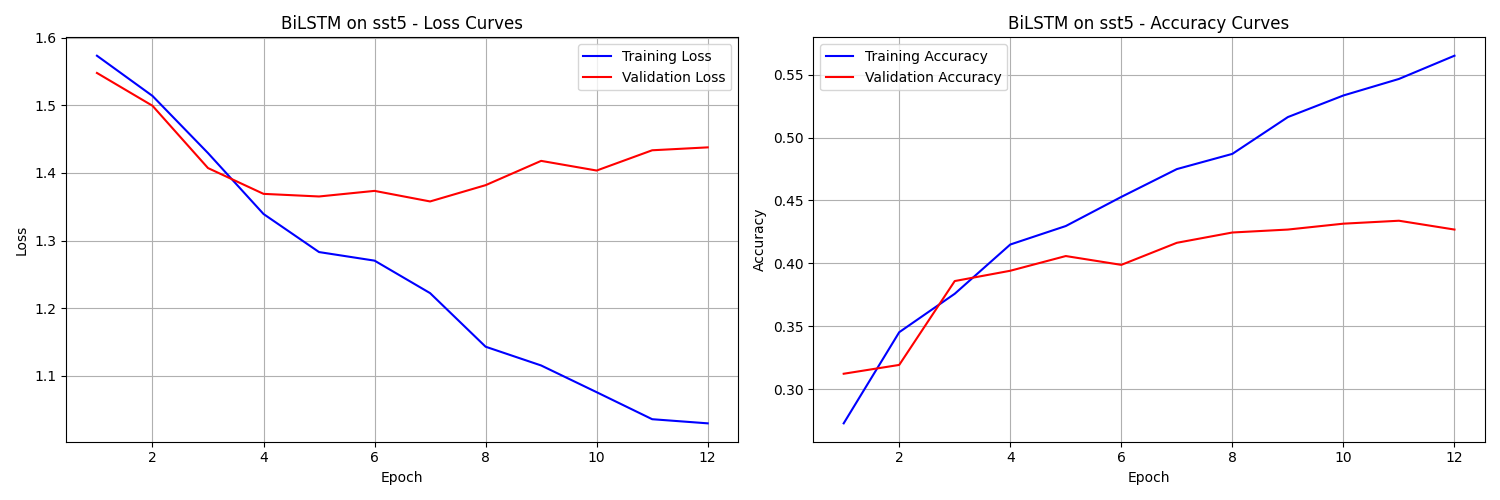
\includegraphics[width=0.9\textwidth, height=0.26\textheight]{figure/plots/BiLSTM_sst5_training_curves}
    \vspace{-2pt}
    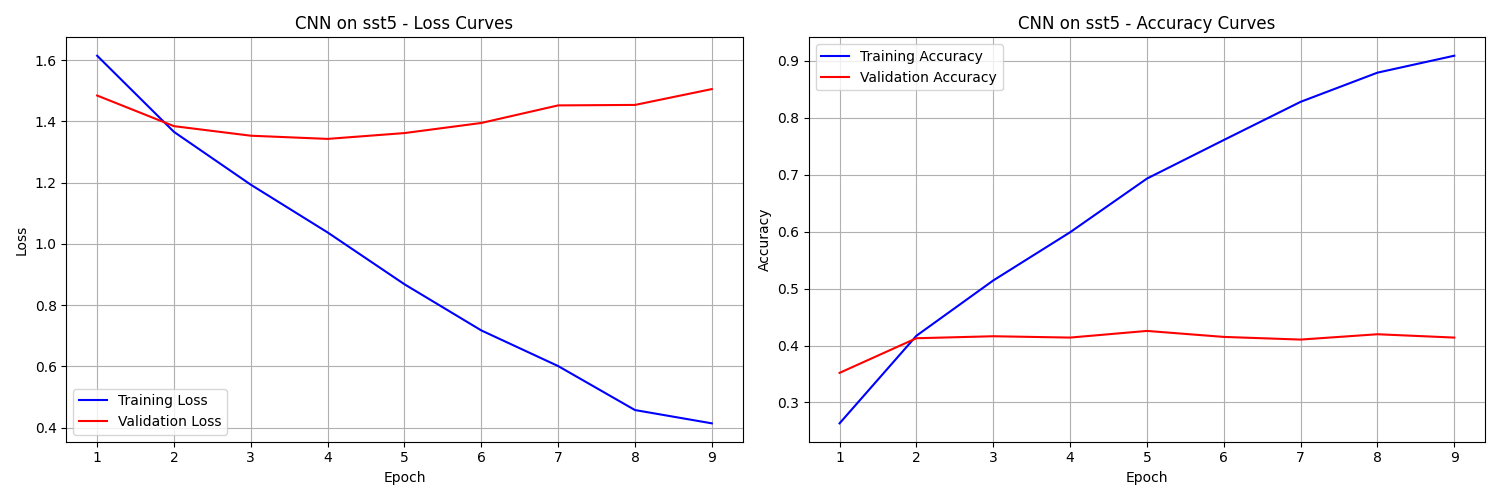
\includegraphics[width=0.9\textwidth, height=0.26\textheight]{figure/plots/CNN_sst5_training_curves}
    \vspace{-2pt}
    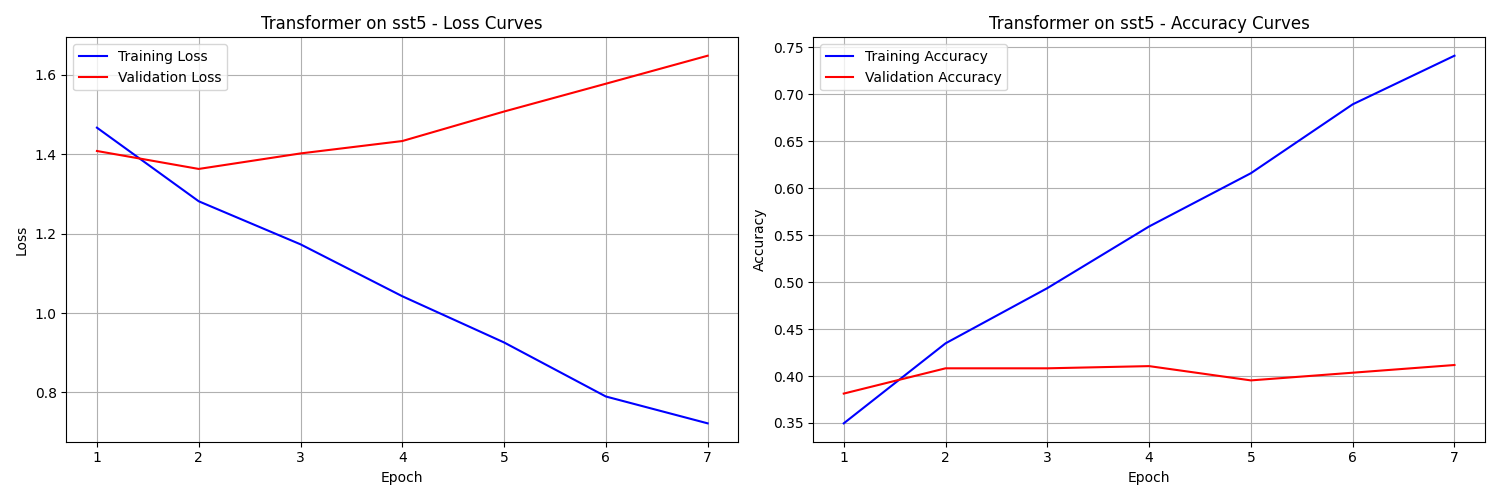
\includegraphics[width=0.9\textwidth, height=0.26\textheight]{figure/plots/Transformer_sst5_training_curves}
    \captionof{figure}{三种模型在 SST-5 上的训练与验证曲线（自上而下：BiLSTM、CNN、Transformer）}
\end{column}
\begin{column}{0.3\textwidth}
\begin{table}[H]
    \centering
    \scriptsize
    \begin{tabular}{lc}
        \toprule
        \multicolumn{2}{c}{\textbf{数据划分}} \\
        \midrule
        训练集 & 7{,}689 \\
        验证集 & 855 \\
        测试集 & 2{,}210 \\
        \bottomrule
    \end{tabular}
\end{table}
\begin{enumerate}
    \fontsize{7pt}{9pt}\selectfont
    \setlength{\itemsep}{2pt}
    \item 三模型 41.9\%--42.4\%，差距远小于统计噪声（标准误约 $\pm$1.1\%）；与文献中非预训练模型的基线水平（42\%--48\%）一致，\textbf{任务难度成为主导因素}；
    \item 加权 F1（37\%--39\%）系统性低于准确率：样本较少的两个极端情感档（very negative / very positive）被忽略，类别不均衡效应明显；
    \item 程度副词（very、too 等）被停用词表过滤，对五级细粒度情感判别不利——\textbf{预处理选择与任务粒度存在交互}，这是粗粒度任务上无害的设计在此处的代价.
\end{enumerate}
\end{column}
    \end{columns}
\end{frame}
\subsection{性能差异的总结}
\begin{frame}\frametitle{模型性能对比总结}
\begin{table}[H]
    \centering
    \small
    \begin{tabular}{lcccc}
        \toprule
        \textbf{测试准确率} & IMDB & AG News & BBC News & SST-5 \\
        \midrule
        BiLSTM & 87.3\% & \textbf{92.3\%} & 94.8\% & 41.9\% \\
        CNN & \textbf{88.5\%} & 92.2\% & \textbf{97.3\%} & \textbf{42.4\%} \\
        Transformer & 88.1\% & 92.1\% & 96.3\% & \textbf{42.4\%} \\
        \bottomrule
    \end{tabular}
\end{table}
\begin{itemize}
    \fontsize{8pt}{10pt}\selectfont
\item \textbf{CNN 最为稳健}：四个数据集上两项第一、两项并列或接近第一，且推理吞吐始终最高.局部 n-gram 特征对关键词与情感短语驱动的分类任务具有高判别价值，归纳偏置与任务高度契合.
\item \textbf{Transformer 的表现随有效上下文增加而提升}：在长文本任务（IMDB、BBC）上接近 CNN，但长序列下自注意力的 $\mathcal{O}(n^2)$ 开销使其推理吞吐降至最低；在小规模、无预训练的设定下未体现全局建模的优势上限.
\item \textbf{BiLSTM 的弱点集中于小样本场景}：BBC（980 条训练样本）上落后 2.5 个百分点，顺序计算也限制其吞吐；在数据充足的 AG News 上则与并行架构持平.
\item \textbf{任务性质决定差距大小}：AG News 与 SST-5 上三模型差距均小于统计噪声，应表述为无显著差异——前者因任务简单（关键词可分），后者因任务过难（五级细粒度），架构差异均被掩盖.
\item \textbf{参数量与性能不成正比}：非嵌入参数量为 BiLSTM 83.6万 $>$ CNN 45.2万 $>$ Transformer 37.1万（嵌入层三者同为词表$\times$300）.参数最多的 BiLSTM 仅在统计平局的 AG News 上名义居首，在 IMDB、BBC、SST-5 上均居末位；本实验小型配置下 Transformer 反而最轻量——性能差异应归因于归纳偏置与任务的契合度，而非模型容量.
\end{itemize}
\end{frame}

\subsection{性能差异的原理分析}
\begin{frame}\frametitle{性能差异的原理分析}
\begin{columns}
    \begin{column}{0.6\textwidth}
            \begin{figure}[H]
                \centering
                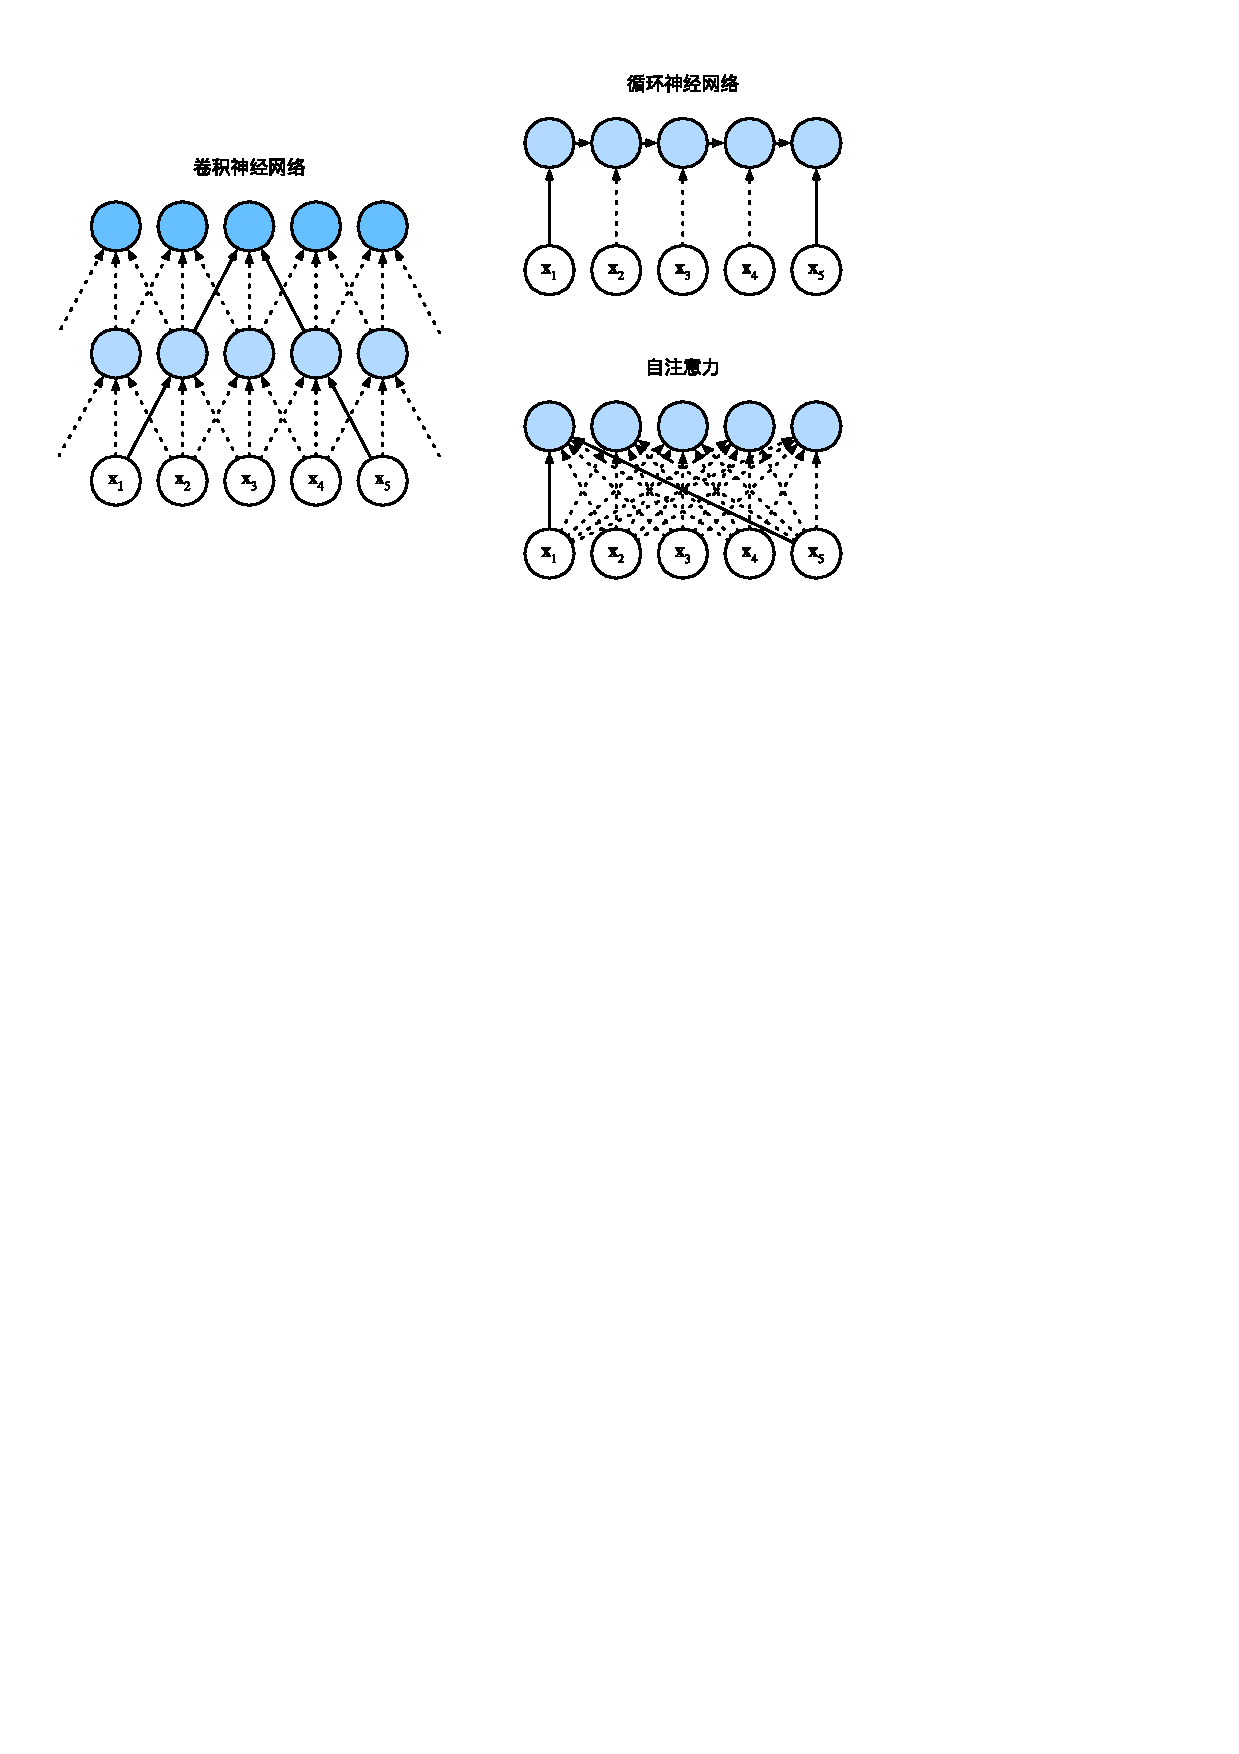
\includegraphics[width=\textwidth, height=0.64\textheight]{figure/cnn-rnn-self-attention}
                \caption{CNN、RNN 与自注意力的连接方式对比}\label{fig:figure}
            \end{figure}
    \end{column}
    \begin{column}{0.4\textwidth}
    \begin{enumerate}
    \item 传统的循环神经网络由于计算具有顺序性，难以实现并行处理；
    \item 卷积神经网络虽可并行计算各位置的隐藏表示，提升计算效率，但在建模远距离依赖时表现受限，因为操作次数随位置间距增加而增长；
    \item Transformer编码器摒弃循环与卷积结构，主要依赖自注意力机制建模输入序列内部的全局依赖关系，显著增强并行能力和长距离依赖建模效果.
    \end{enumerate}
    \end{column}
    \end{columns}
\newpage
\begin{enumerate}
    \item 每层复杂度：指网络中每一层在处理输入序列时所需的总计算量；
    \item 最小顺序操作数：指完成前向传播所需的最小顺序计算步骤数，反映了模型并行化的潜力.\textbf{该指标越小，模型在硬件上越容易实现高效并行}；
    \item 最大路径长度：指在网络结构中，任意输入位置与任意输出位置之间信息传播所需经过的最长路径长度（操作步数）.\textbf{路径越短，模型越容易捕捉长距离依赖关系，对于处理长序列任务具有优势}.
\end{enumerate}
受限自注意力仅考虑输入序列中以各输出位置为中心、大小为$r$的邻域范围，可提高涉及超长序列任务的计算性能.\footcite{vaswaniAttentionAllYou2017}
\begin{table}[H]
    \centering
    \caption{不同层类型的计算复杂度与路径特性}
    \label{tab:layer-comparison}
    \begin{tabular}{lccc}
        \toprule
        层类型 & 每层复杂度 & 最小顺序操作数 & 最大路径长度 \\
        \midrule
        自注意力层 & $\mathcal{O}(n^2 \cdot d)$ & $\mathcal{O}(1)$ & $\mathcal{O}(1)$ \\
        循环层 & $\mathcal{O}(n \cdot d^2)$ & $\mathcal{O}(n)$ & $\mathcal{O}(n)$ \\
        卷积层（空洞/层级） & $\mathcal{O}(k \cdot n \cdot d^2)$ & $\mathcal{O}(1)$ & $\mathcal{O}(\log_k n)$ \\
        受限自注意力层 & $\mathcal{O}(r \cdot n \cdot d)$ & $\mathcal{O}(1)$ & $\mathcal{O}(n / r)$ \\
        \bottomrule
    \end{tabular}
\end{table}
\begin{enumerate}
\fontsize{9pt}{11pt}\selectfont
\item 自注意力层连接所有位置仅需常数次数的顺序操作，循环层则需 $\mathcal{O}(n)$ 次.
\item 计算复杂度对比：
\begin{itemize}
\item 当序列长度 $n$ 小于特征维度 $d$ 时，自注意力层的每层复杂度低于循环层；该条件在短文本或较大隐藏维度配置下更常见.
\end{itemize}
\item 单个卷积层若核宽度 $k < n$，无法直接连接所有输入与输出位置.
\begin{itemize}
\item 普通连续卷积需堆叠 $\mathcal{O}(n/k)$ 层.
\item 空洞卷积或层级卷积可将路径长度降至 $\mathcal{O}(\log_k n)$.
\end{itemize}
\item 卷积层计算成本通常比循环层高 $k$ 倍.
\begin{itemize}
\item 可分离卷积显著降低复杂度至 $\mathcal{O}(k \cdot n \cdot d + n \cdot d^2)$.
\item 即使 $k=n$，可分离卷积复杂度仍与自注意力层加逐位前馈层相当.
\end{itemize}
\item 对超长序列任务，可限制自注意力的邻域范围为大小 $r$ 的窗口，计算性能提升，但最大路径长度增至 $\mathcal{O}(n/r)$.
    \end{enumerate}
\textbf{本实验的实证对应}（推理吞吐量，samples/s）：
\begin{itemize}
    \fontsize{9pt}{11pt}\selectfont
    \item 短序列（AG News，$n=64 < d_{\mathrm{model}}=128$）：自注意力的 $\mathcal{O}(n^2 d)$ 低于循环层的 $\mathcal{O}(n d^2)$，Transformer（30.0万）接近 CNN（34.2万），远高于 BiLSTM（17.2万）；
    \item 长序列（BBC News，$n=512 > d=128$，$n/d=4$）：自注意力的 $\mathcal{O}(n^2 d)$ 开始超过循环层的 $\mathcal{O}(n d^2)$，Transformer 降至三者最低（约 2.0万），被顺序计算的 BiLSTM（2.7万）反超——理论复杂度表与实测吞吐的相对关系一致.
\end{itemize}
\end{frame}

\subsection{全文总结与模型建议}
\begin{frame}\frametitle{全文总结与模型建议}
\centering
    \begin{columns}[T]
        \column{0.30\textwidth}
        \begin{block}{CNN}
    \fontsize{8pt}{9pt}\selectfont
    \begin{enumerate}
        \item 擅长提取局部特征，适用于关键词驱动的任务
        \item 参数较少，训练速度快，资源开销低
        \item 短文本分类效果较好
        \item 易并行，计算效率高
    \end{enumerate}
    \begin{enumerate}
        \item 难以捕捉长距离依赖
        \item 全局语义建模能力不足
        \item 依赖固定输入长度，可能引入截断或填充误差
    \end{enumerate}
\end{block}

\column{0.30\textwidth}
\begin{block}{LSTM}
    \fontsize{8pt}{9pt}\selectfont
    \begin{enumerate}
        \item 能捕捉中长期序列依赖，适合变长输入
        \item 顺序建模能力强，适用于时间序列和语言任务
        \item 数据充足时与并行架构表现相当（如本实验 AG News）
    \end{enumerate}
    \begin{enumerate}
        \item 顺序计算限制并行性，训练与推理效率低
        \item 长序列处理仍存在梯度消失或爆炸风险（需配合梯度裁剪）
        \item 样本效率较低，小样本场景下易过拟合、泛化最差（如本实验 BBC News）
    \end{enumerate}
\end{block}

\column{0.30\textwidth}
\begin{block}{Transformer}
    \fontsize{8pt}{9pt}\selectfont
    \begin{enumerate}
        \item 能有效建模长距离依赖，适用于复杂语义分析
        \item 训练阶段可高度并行，提高训练效率
        \item 自注意力机制可动态关注关键信息
        \item 架构灵活，可拓展至大规模预训练模型
    \end{enumerate}
    \begin{enumerate}
        \item 大规模配置下参数量与训练成本高（本实验小型配置的非嵌入参数量反而最少，约 37 万）
        \item 对数据规模和质量较为敏感，易过拟合
        \item 长序列下自注意力 $\mathcal{O}(n^2)$ 开销显著（如本实验 BBC News 推理吞吐最低）
    \end{enumerate}
\end{block}
    \end{columns}

    \begin{block}{模型选择建议}
        \fontsize{8pt}{9pt}\selectfont
        \begin{enumerate}
            \setlength{\itemsep}{1pt}
            \item 数据规模小、文本较短：优先考虑 CNN，训练高效、表现稳定；
            \item 数据规模大、计算资源充足：优先考虑 Transformer，通常具备更高性能上限；
            \item 对顺序信息较敏感、文本中等长度：可选择 LSTM，兼顾建模能力与稳定性；
            \item 实际任务中可融合多种架构，如 CNN+LSTM 或 BERT+CNN 等实现性能提升.
        \end{enumerate}
    \end{block}

    \begin{block}{补充说明}
        \fontsize{8pt}{9pt}\selectfont
        \begin{enumerate}
            \setlength{\itemsep}{1pt}
            \item Transformer 架构（如 BERT）在多数文本分类基准中表现突出，已成为主流方法；
            \item CNN、LSTM 在中小型数据集、特定领域（如医学、金融文本）中仍具竞争力，且资源消耗低；
            \item 模型选择应综合考虑数据特征、业务需求、可用算力与部署效率等多因素.
        \end{enumerate}
    \end{block}
\end{frame}

\section{附录}
\begin{frame}\frametitle{参考文献}
\scriptsize
    \printbibliography[heading=subbibliography,title={参考文献}]
\end{frame}

% \subsection{部分代码}
% \begin{frame}\frametitle{文本预处理}
%     \lstinputlisting[label={lst:lstinputlisting1}]{../Code/src/data/preprocessor.py}
% \end{frame}
% \begin{frame}\frametitle{词嵌入层}
%     \lstinputlisting[label={lst:lstinputlisting2}]{../Code/src/data/embeddings.py}
% \end{frame}
% \begin{frame}\frametitle{基础模型类}
%     \lstinputlisting[label={lst:lstinputlisting3}]{../Code/src/models/base.py}
% \end{frame}
% \begin{frame}\frametitle{BiLSTM文本分类模型}
%     \lstinputlisting[label={lst:lstinputlisting4}]{../Code/src/models/bilstm.py}
% \end{frame}
% \begin{frame}\frametitle{CNN文本分类模型}
%     \lstinputlisting[label={lst:lstinputlisting5}]{../Code/src/models/cnn.py}
% \end{frame}
% \begin{frame}\frametitle{Transformer文本分类模型}
%     \lstinputlisting[label={lst:lstinputlisting6}]{../Code/src/models/transformer.py}
% \end{frame}
% \begin{frame}\frametitle{训练配置}
%     \lstinputlisting[label={lst:lstinputlisting7}]{../Code/src/config.py}
% \end{frame}

\setbeamertemplate{background canvas}[vertical shading][bottom=white,top=blue!20]
\begin{frame}
    \begin{center}
        {\huge \textcolor[rgb]{0.50,0.00,1.00}{\rmfamily{感谢各位，敬请批评指正！}}}
    \end{center}
\end{frame}
\end{document}
